\chapter{Results and Evaluation}
\label{chap:results}

This chapter presents the synthesis of comprehensive study, experimentation, and analysis of data obtained from the CardioSync and Reference Freebie systems \cite{de2022Intermittently}. The results of this study provide valuable information on the intricate relationship between the precision of synchronisation, specifically in terms of \textit{the time it takes to establish a BLE connection, and power and energy consumption}. This is in comparison to a reference system that does not employ any synchronisation mechanism. 

\noindent Guided by the set of well-defined research goals, this chapter aims to navigate through assessments, unveiling the accuracy, efficiency, and practical implications of the system. So this chapter is strictly weaved with the research goals and divided into further sections, which present results that collectively answer the research questions.

\section{Revisiting Research Goals}
\begin{enumerate}
    \item \textbf{Evaluation of Heart Rate Sensor and Synchronization Algorithm:}
    \begin{itemize}
        \item The central objective of this thesis is to bridge the gap between intermittent operation and efficient connectivity through the utilization of an external clock signal—specifically, the human body's heart rate. Therefore, the integration of the MAX30102 heart rate sensor and its associated algorithm is the cornerstone of this synchronisation solution. 
        \item Therefore, before we embark on the detailed examination of the performance of the CardioSync system, we critically evaluate the MAX30102 heart rate sensor and its algorithm for accuracy, robustness, and successful integration into our battery-less framework.
    \end{itemize}

    \item \textbf{Evaluation of Integrated CardioSync system:}
    \begin{itemize}
        \item It is vital to assess the working of the system with relevant measurements of current and voltage that shows the expected working of the sensor integration in battery less framework.
        \item To fulfil this, the system is subjected to the test for synchronised BLE connection between two batteryless devices with Continuous and Intermittent voltage supply, achieved through a square wave pattern simulation.
    \end{itemize}

    \item \textbf{Comparative Analysis against Reference Design:}
    \begin{itemize}
        \item Bench-marking the efficiency of the final integrated CardioSync system against the existing reference system of FreeBie, on \textit{Connection setup time, Power and Energy}, marks the final and important aspect of this thesis.
        \item It draws out valuable implications about the CardioSync systems as juxtaposed with reference design in three different BLE configurations with different energy usage.
    \end{itemize}
\end{enumerate}

\noindent To seek assertive evidence for achievement of our goals, we meticulously conducted a series of experiments in controlled environments with necessary devices and analysers. In the following sections, we discuss those experiments, observations, inference, and results elaborately.



\section{Evaluation of Heart Rate Sensor and Synchronization Algorithm:}
The evaluation in this section assesses the Sensor and heart beat detection algorithm and it is split into two parts - \textit{Sensor accuracy profiling} based on phase difference for a particular peak detected between two sensors and \textit{BLE connection performance} at different sensor sampling rate.

\subsection{Sensor Accuracy Profiling}
Sensor accuracy to detect heart beat is mainly based on the peak detection algorithm developed for this thesis, and also on the configurations of the sensor register. However, in our particular scenario, the sensor was designed to operate in a configuration that minimized power consumption. Consequently, the heart beat detection algorithm was optimized to enhance accuracy. However, a phase difference was observed between the detected peaks, which was measured and the accuracy was assessed at various sampling rates.

\subsubsection{Experimental Setup}
To measure the phase difference between the heart beat detected by two different MAX30102 sensors, a nRF52840DK development board \cite{nRF52840} was used and the sensors are attached to it on GPIO pins.

\noindent The measurement software was developed based on nRF5 SDK \cite{2023nRF5} to interface with two sensor boards using two-wire interface (TWI).  The software would use the heart beat detection algorithm of the CardioSync system to independently identify heart pulse peaks for each sensor and log the corresponding detection time. Subsequently, the phase difference should be computed between the aforementioned peaks. After two sensors have recorded around 250 peak detection, an experiment is finished, and it is repeated four times with four different sensor sampling rates: \textit{25Hz, 50Hz, 100Hz, and 1000Hz}.

\subsubsection{Data Presentation}
The \autoref{fig:histogram_25}, \autoref{fig:histogram_50}, \autoref{fig:histogram_100}, \autoref{fig:histogram_1000}, shows the histogram of phase difference data recorded for different sensor read sampling rates. The next section will discuss these plots to infer the results of accuracy in detecting heart peaks. And the \autoref{tab:phase_difference_comp}, shows the mean, minimum and maximum phase differences recorded at different sampling rates.

\begin{figure}[H]
    \begin{subfigure}{0.5\linewidth}
        \centering
        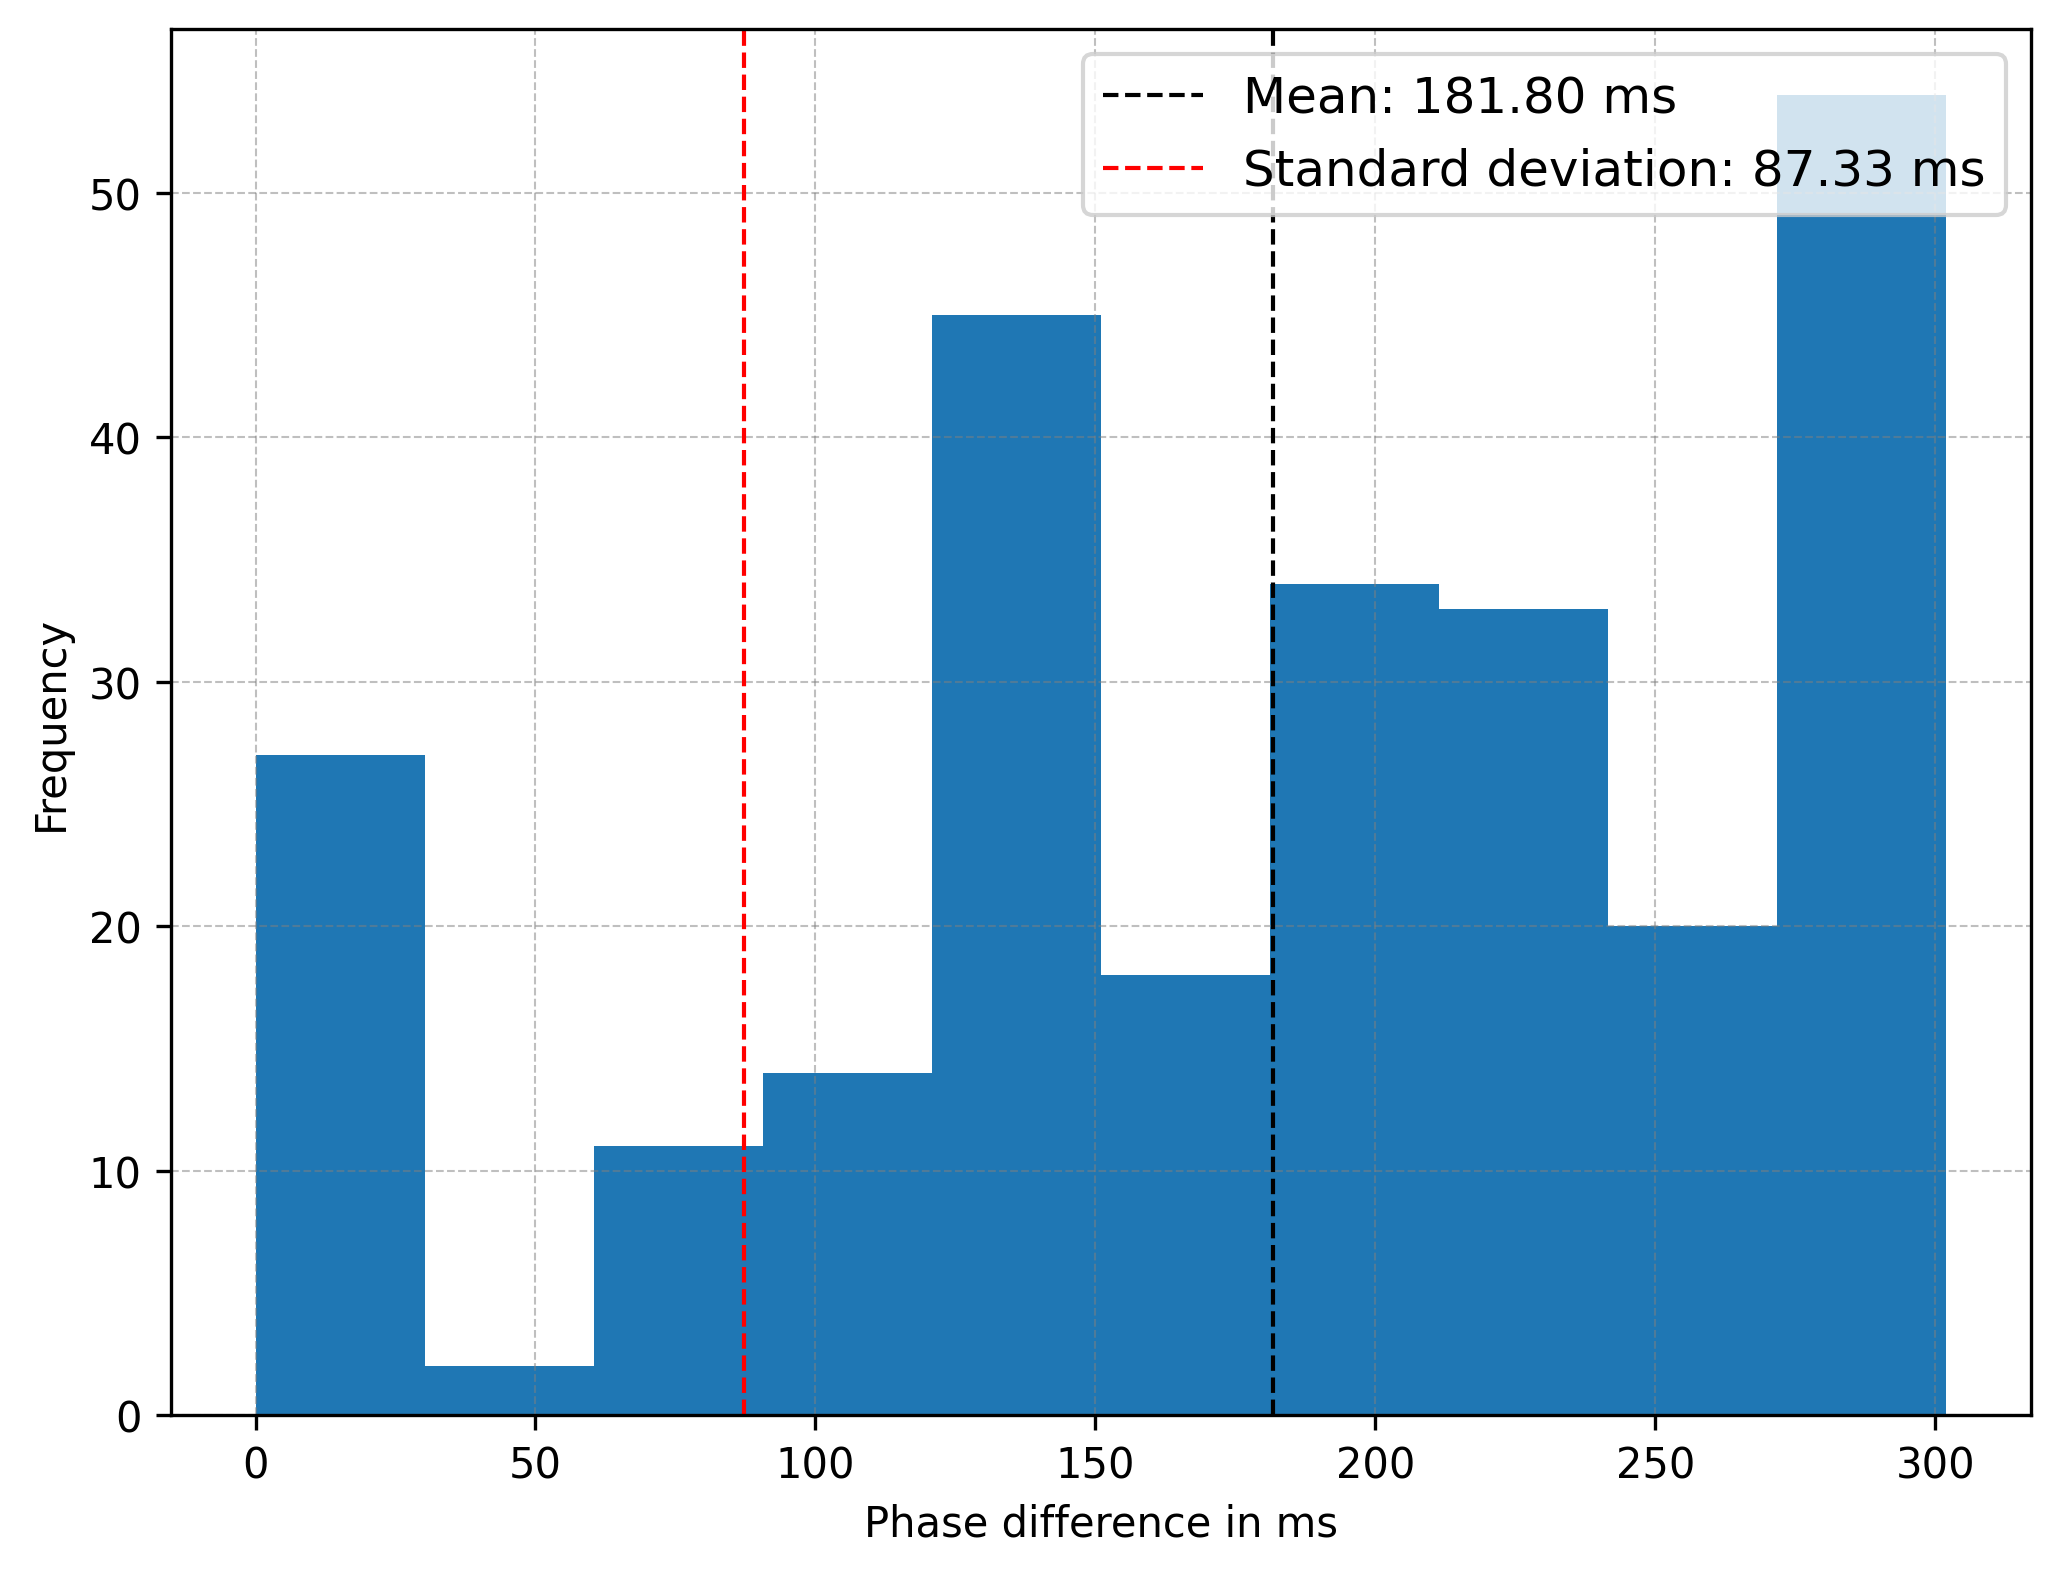
\includegraphics[width=\linewidth]{chapters/Results/histogram_25.png}
        \caption{25Hz}
        \label{fig:histogram_25}
    \end{subfigure}
    \begin{subfigure}{0.5\linewidth}
        \centering
        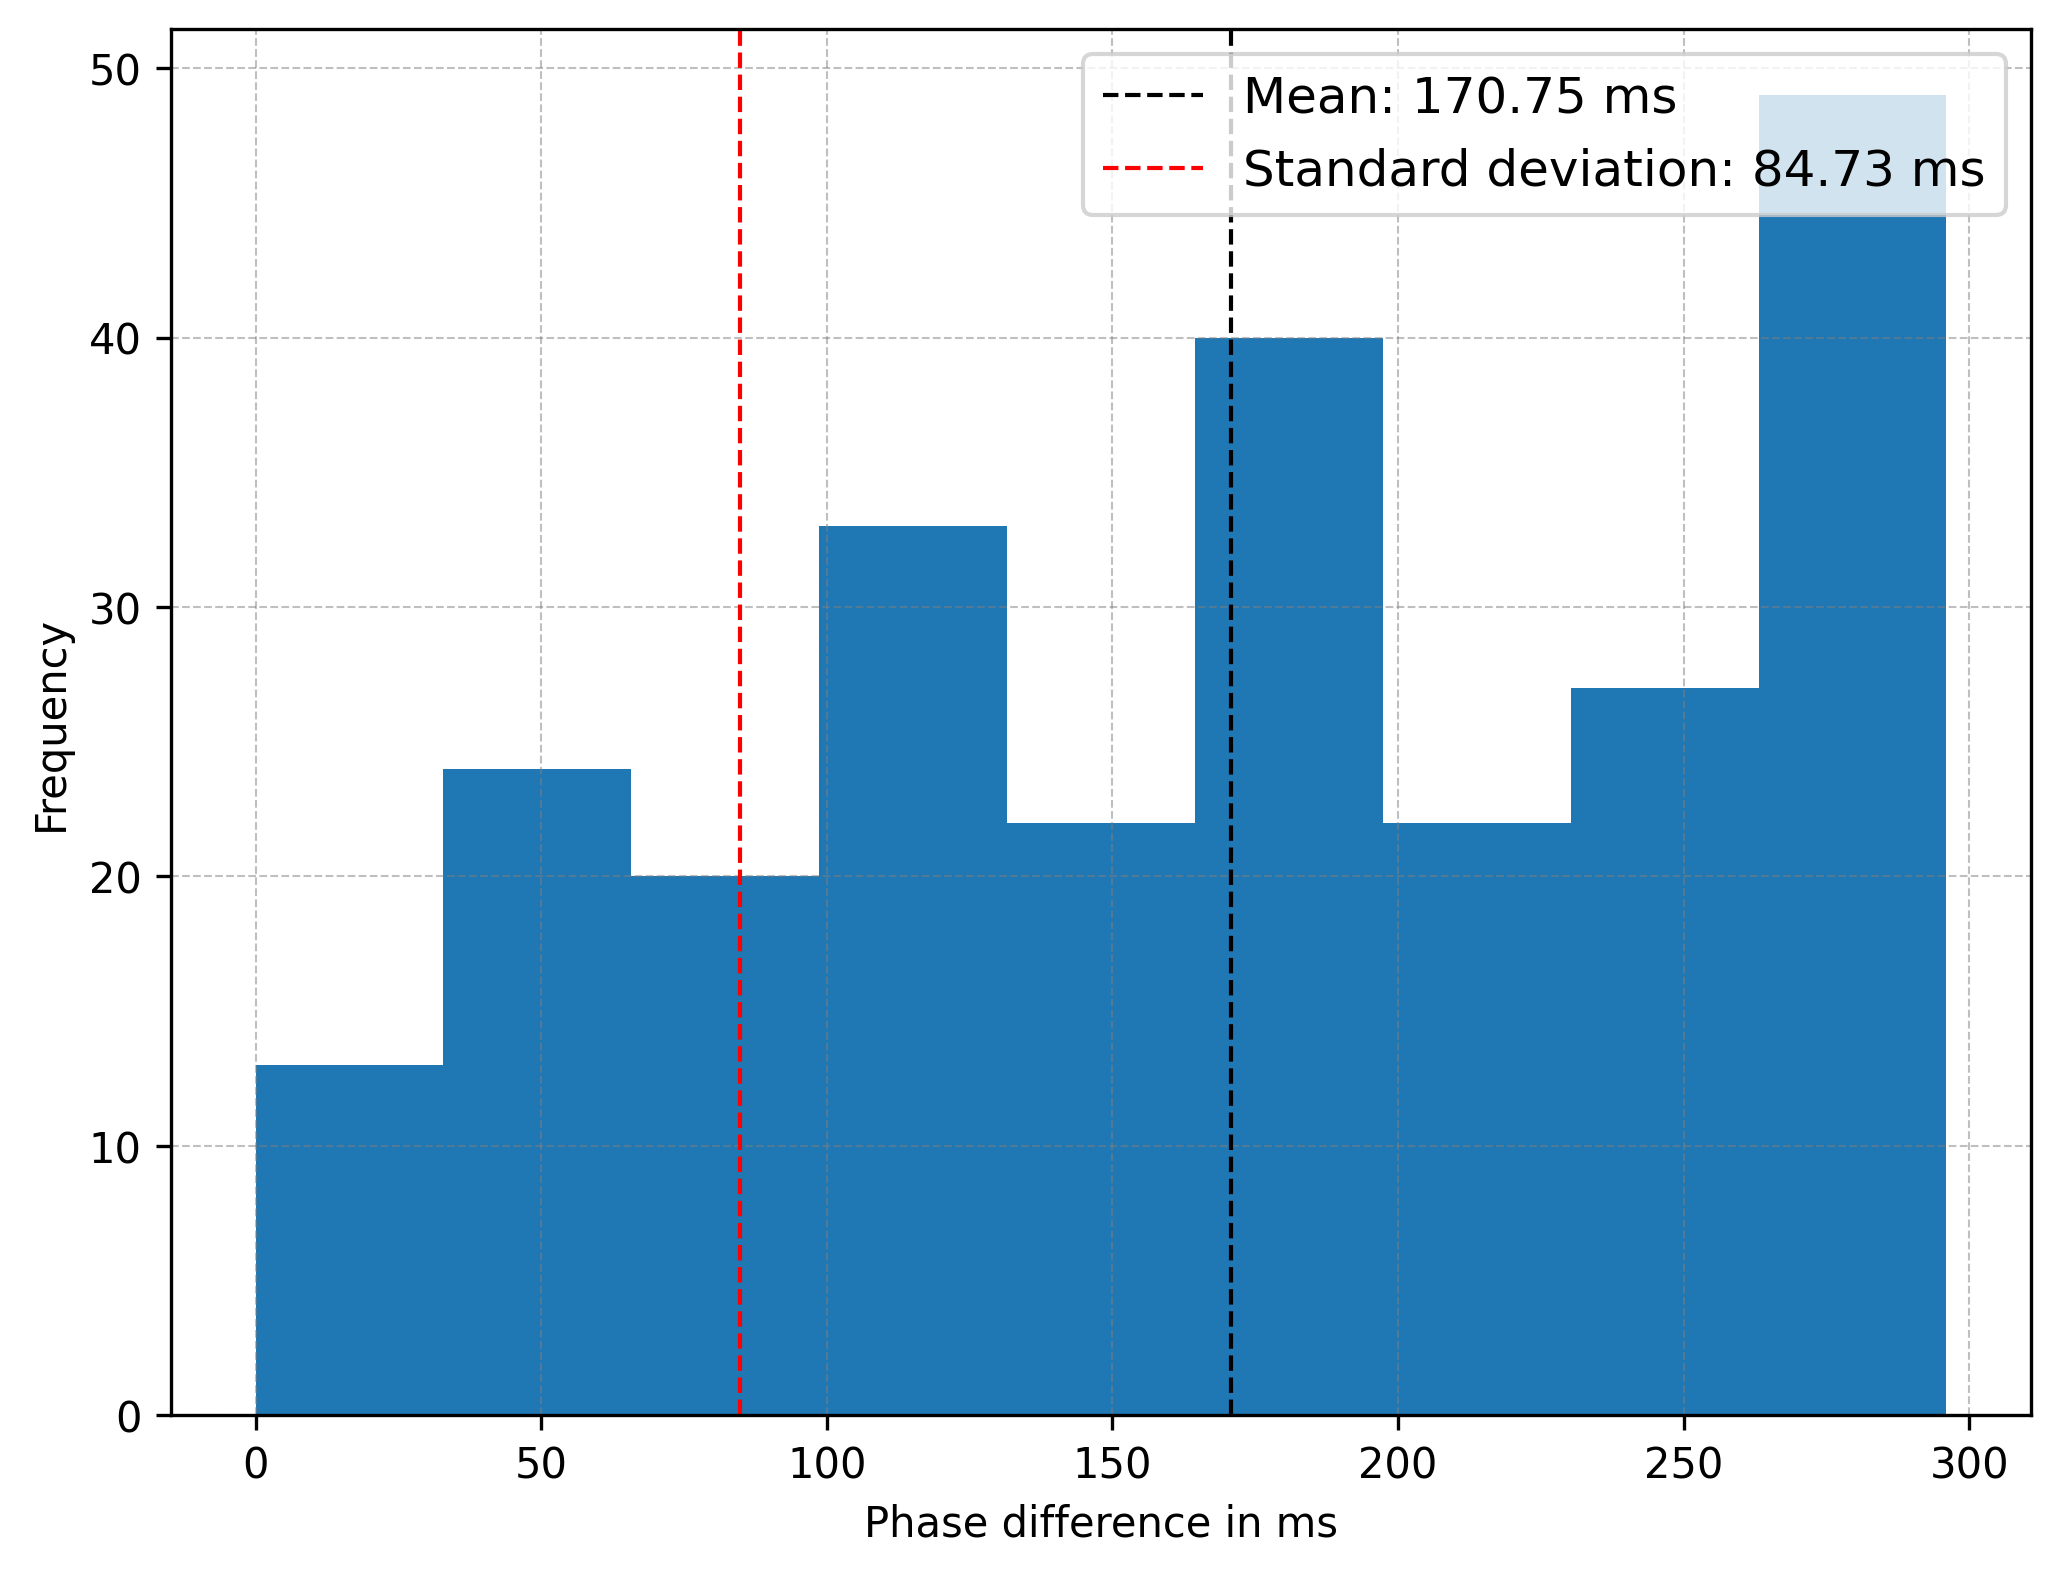
\includegraphics[width=\linewidth]{chapters/Results/histogram_50.png}
        \caption{50Hz}
        \label{fig:histogram_50}
    \end{subfigure}
    \begin{subfigure}{0.5\linewidth}
        \centering
        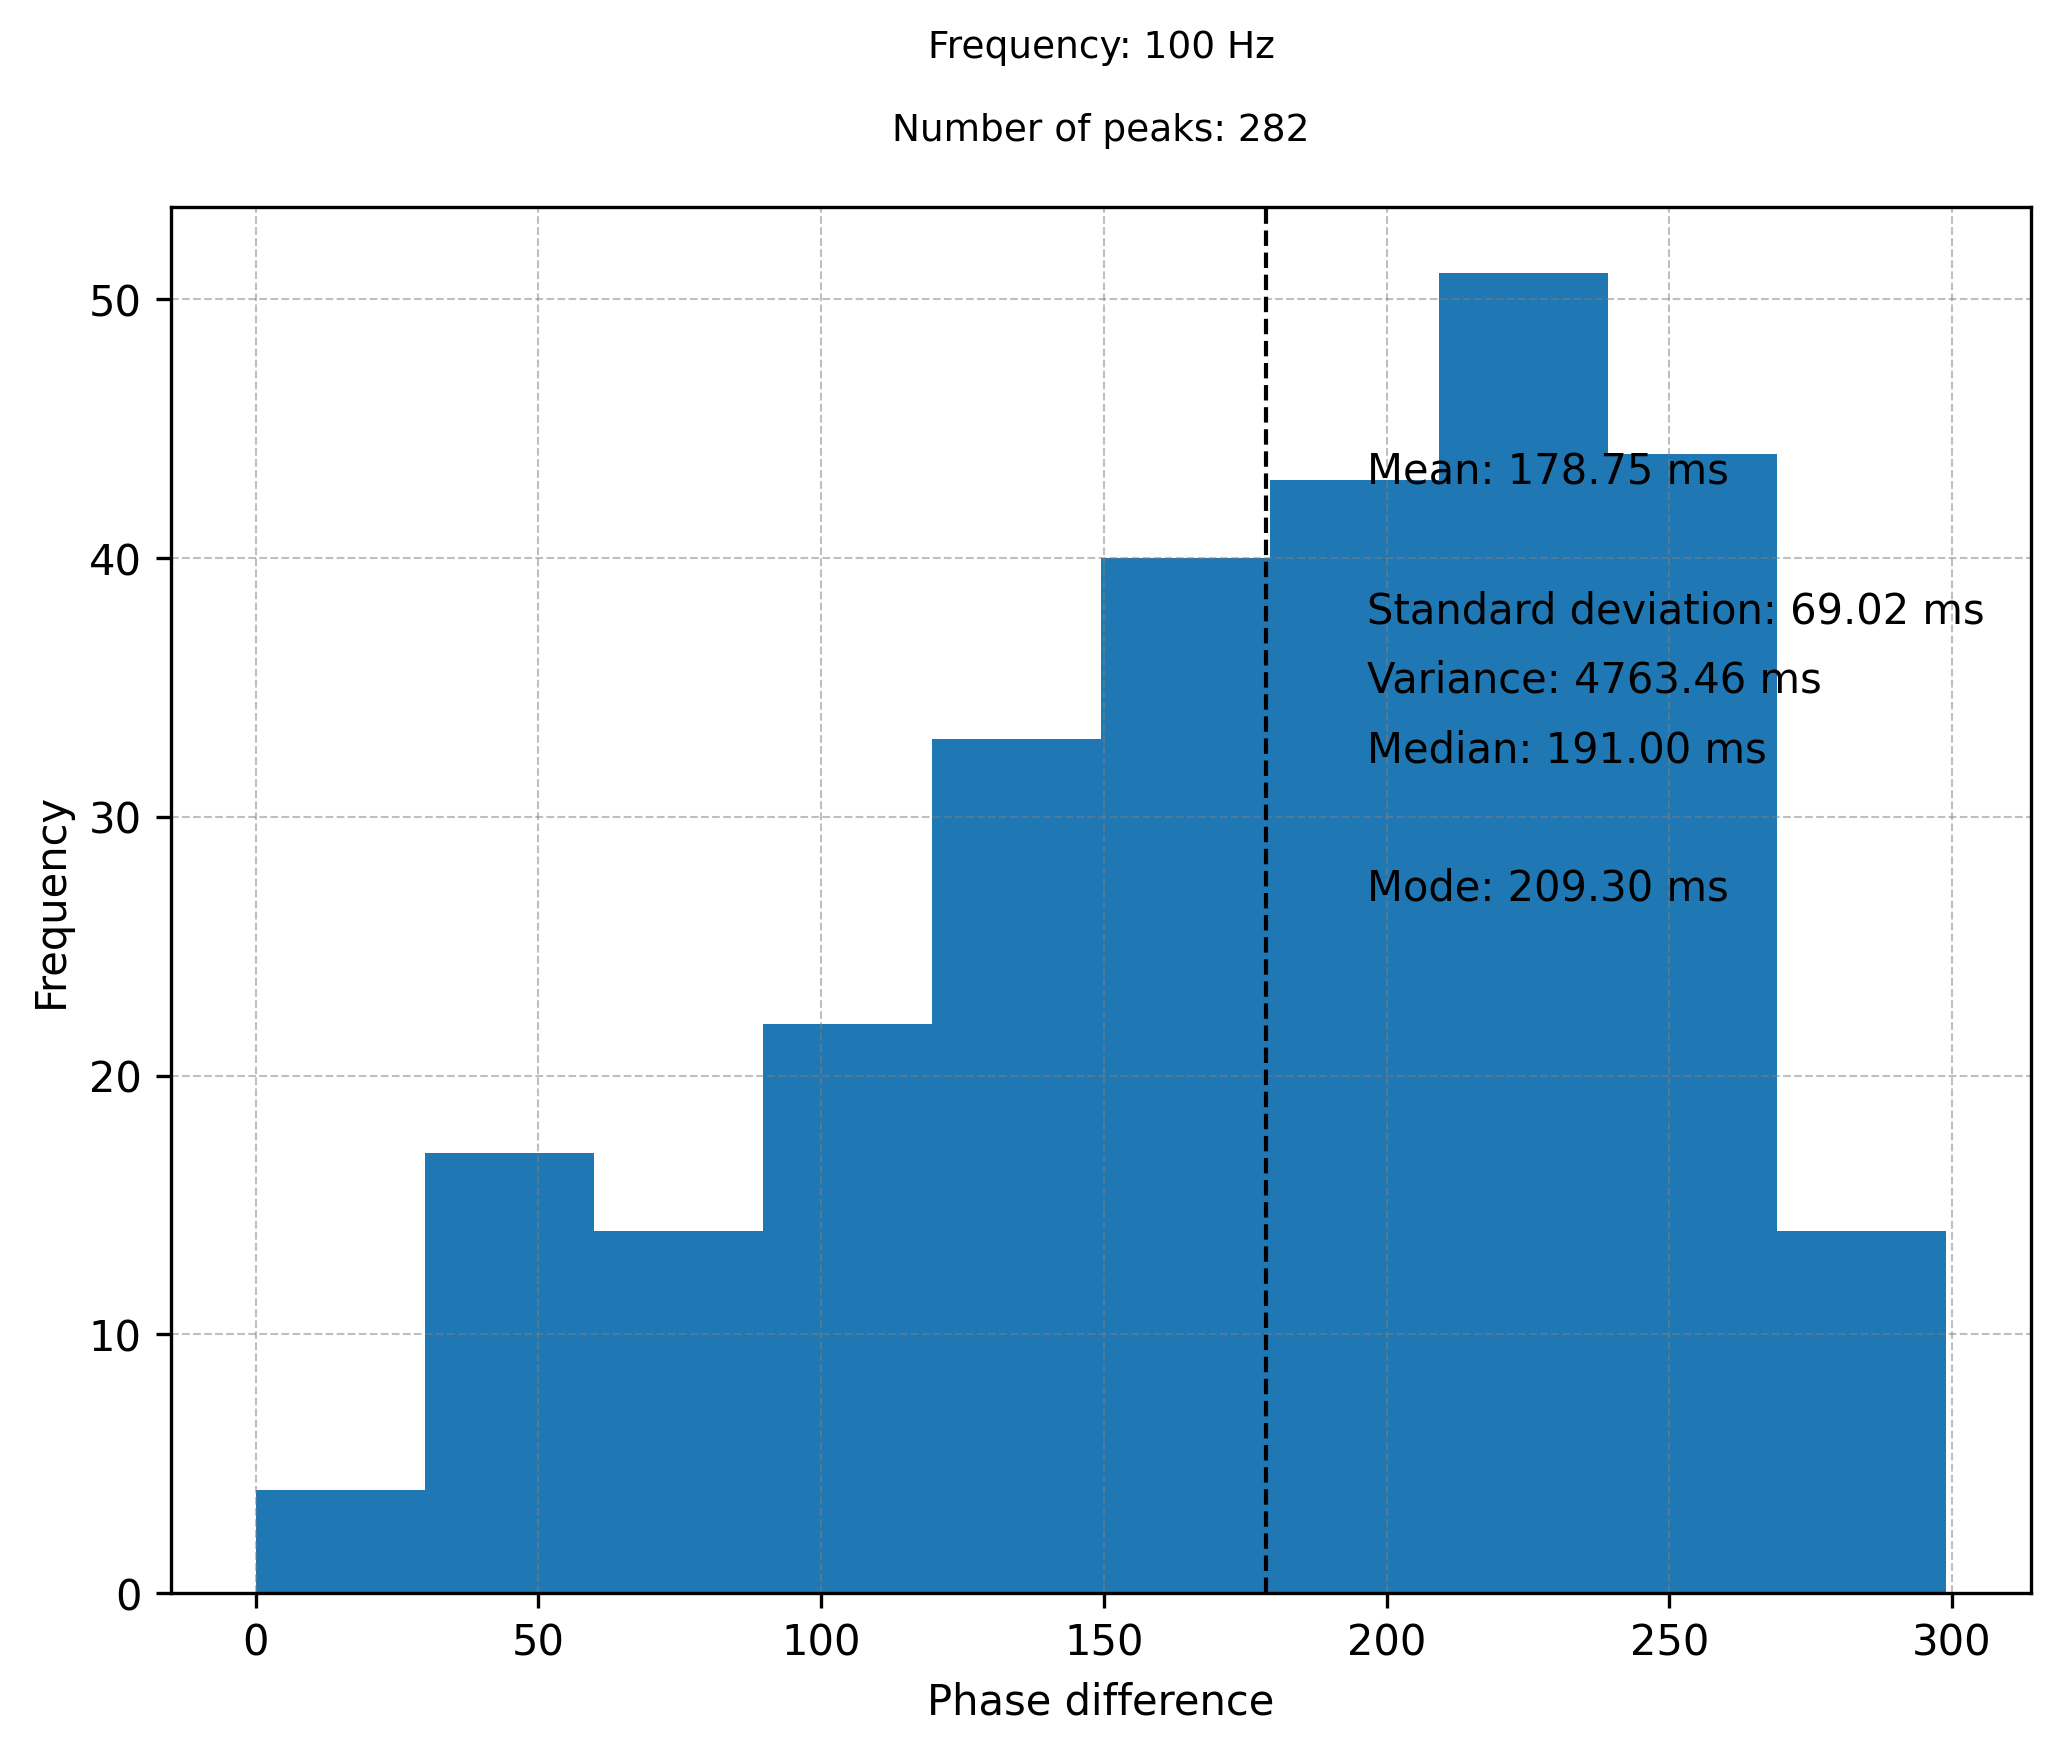
\includegraphics[width=\linewidth]{chapters/Results/histogram_100.png}
        \caption{100Hz}
        \label{fig:histogram_100}
    \end{subfigure}
    \begin{subfigure}{0.5\linewidth}
        \centering
        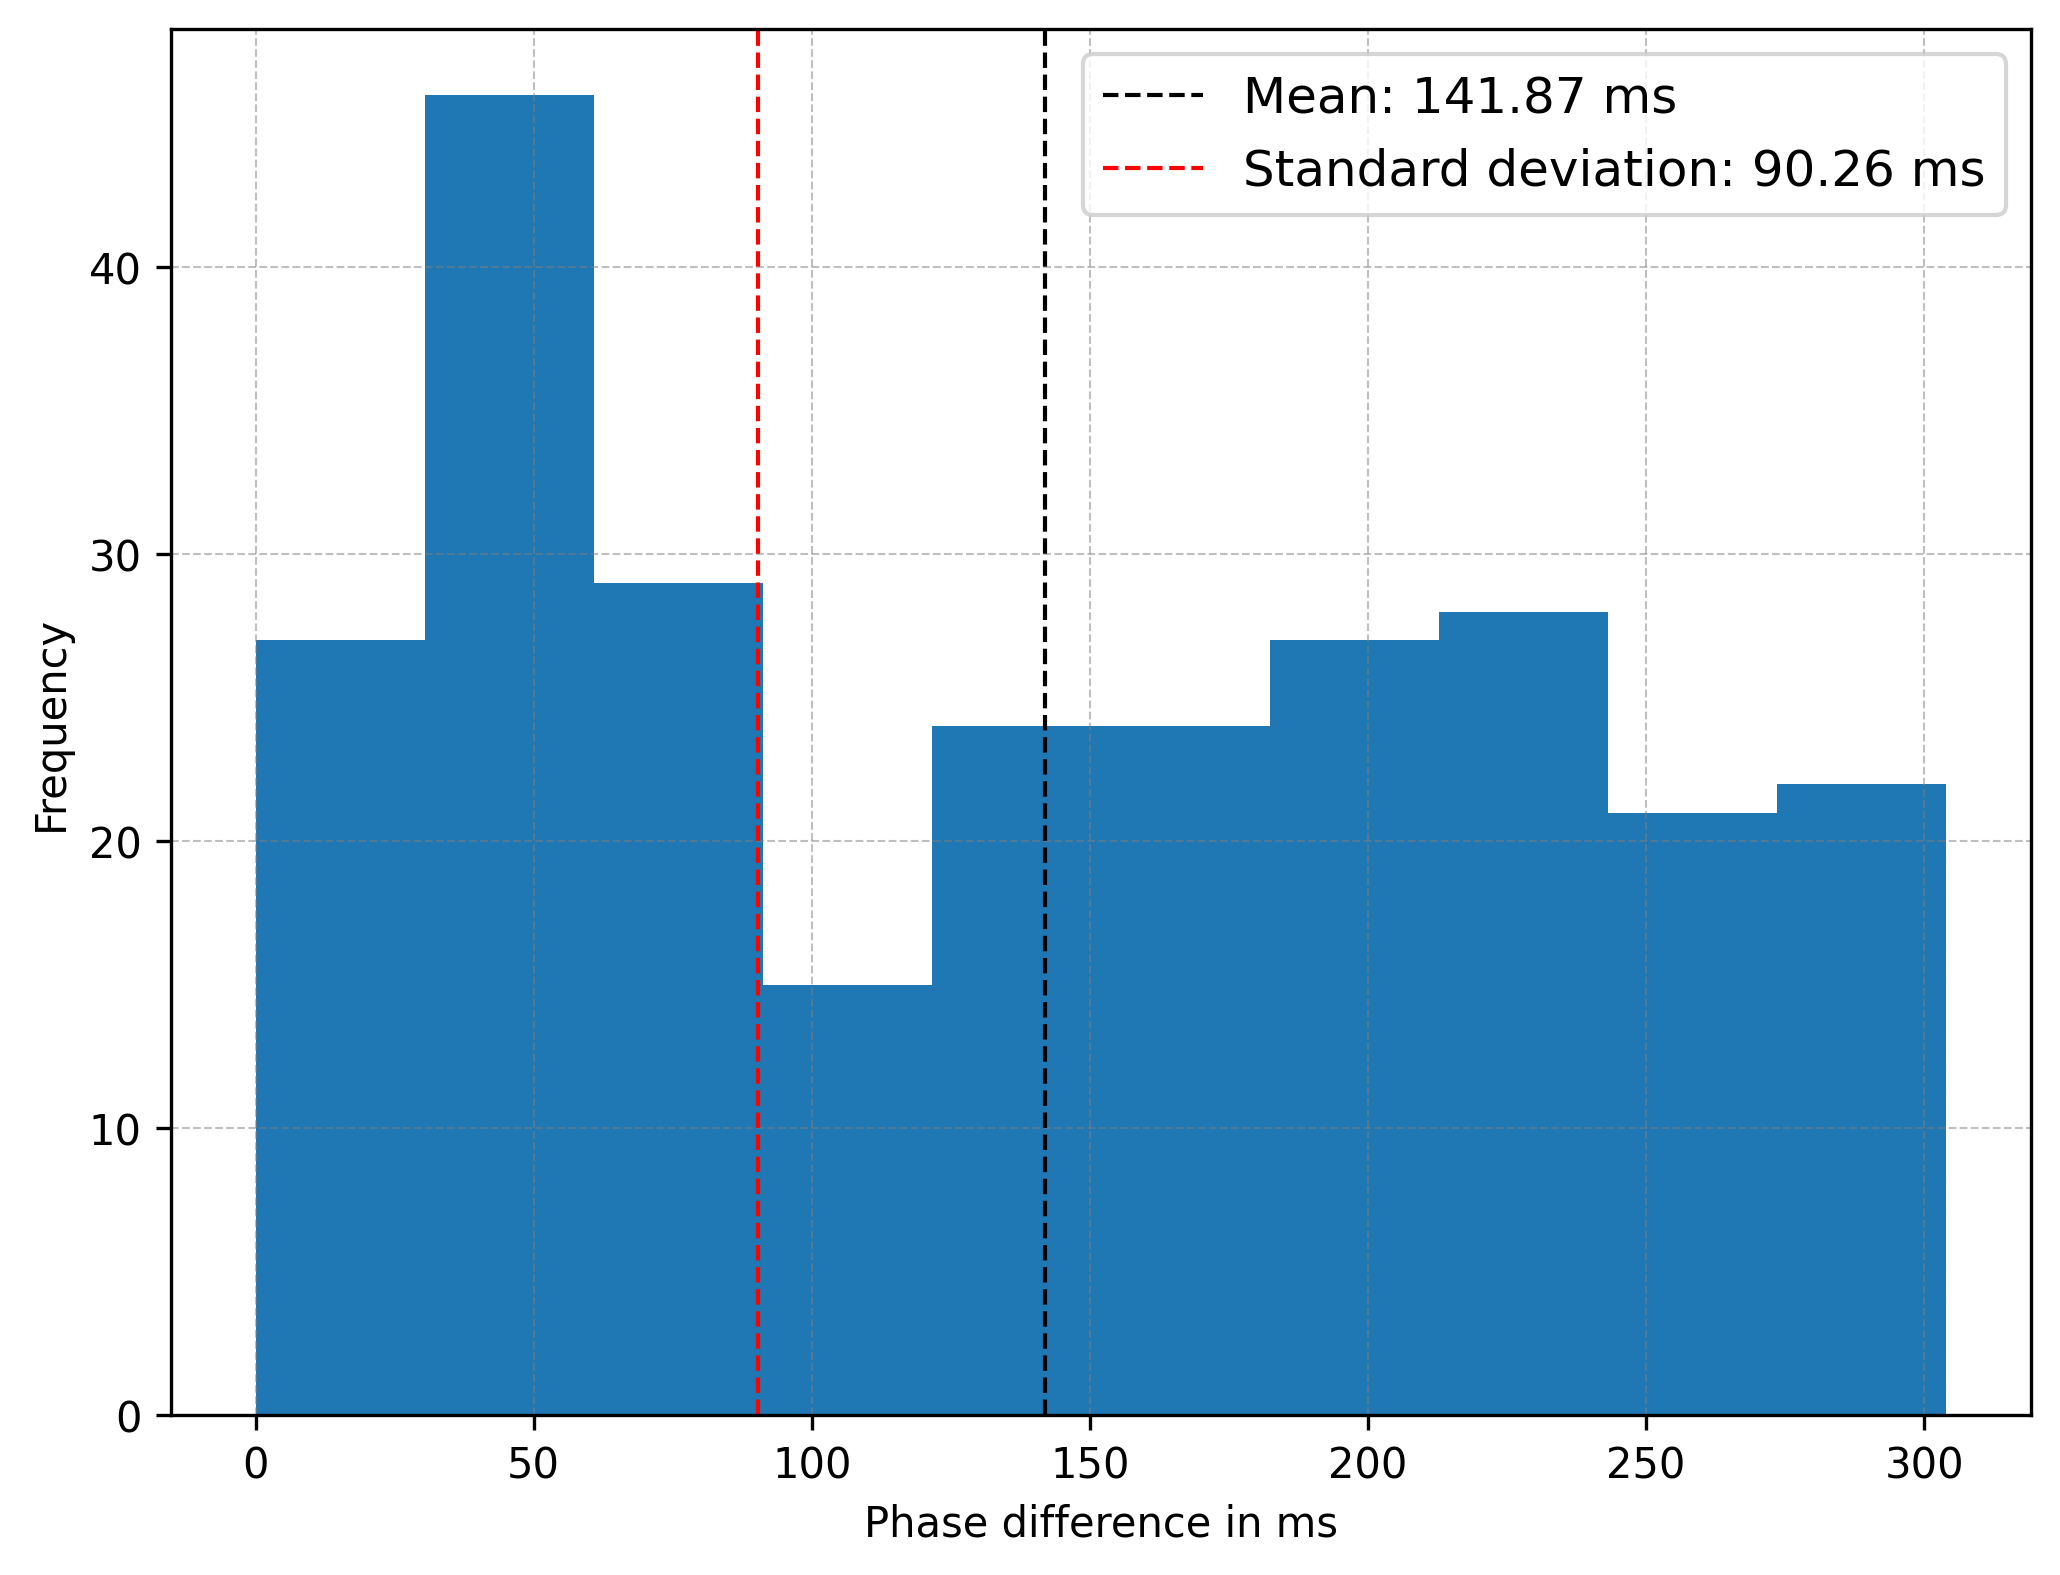
\includegraphics[width=\linewidth]{chapters/Results/histogram_1000.png}
        \caption{1000Hz}
        \label{fig:histogram_1000}
    \end{subfigure}
    \caption{\centering Histogram of Phase differences between heart pulses detected by two sensors recorded at different sensor read frequencies}
\end{figure}

\subsubsection{Interpretation of Results}
Based on the analysis of the histogram data distribution and reviewing of its statistical characteristics, it can be deduced that the occurrence of phase difference in the detection time between two sensors is an unavoidable outcome. However, the data has the potential to assist us in determining the most optimal sensor read frequency for our CardioSync system.

\paragraph{Sampling rate 25Hz}
The distribution of phase differences at the 25Hz sampling rate exhibits a right skew, indicating a higher probability of frequent occurrences of larger phase differences. Furthermore, approximately 33\% detected peaks are completely out of phase (>305ms) and neglected by measuring logic for data collection.

\paragraph{Sampling rate 50Hz}
Similar to 25Hz data, it can seen from the \autoref{fig:histogram_50}, that distribution is right skewed and there is high probability of larger difference. And about 35\% peaks detected are out of phase (>305ms). 

\paragraph{Sampling rate 100Hz}
The figure \ref{fig:histogram_100} shows slightly right skewed normal distribution. It can be inferred that phase differences are likely to occur mostly around the mean value. The approximately 24\% peaks detected are out of phase (>305ms)  

\paragraph{Sampling rate 1000Hz}
The \autoref{fig:histogram_1000} shows an irregular distribution of phase difference, depicting the random occurrence of the phase difference, which is unpredictable. Also, the approximate 20-30\% peaks detected are out of phase (>305ms).

\subsubsection{Conclusive remark}
From all these observations, it can be concluded that \textbf{\textit{Sampling rate 100Hz}} is more predictable in terms of phase difference and is more accurate in heart pulse peak detection between two sensors. Also, even the sensor register settings are at 50 samples per second, thereby not losing any samples from the sensor.

\begin{table}[H]
\centering
\begin{tabular}{|c|ccc|}
\hline
\multirow{2}{*}{\textbf{\begin{tabular}[c]{@{}c@{}}Sensor \\ Sampling rate\end{tabular}}} &
  \multicolumn{3}{c|}{\textbf{\begin{tabular}[c]{@{}c@{}}Phase difference\\ in milliseconds\end{tabular}}} \\ \cline{2-4} 
                 & \multicolumn{1}{c|}{\textbf{Mean}} & \multicolumn{1}{c|}{\textbf{Min}} & \textbf{Max} \\ \hline
\textit{25 Hz}   & \multicolumn{1}{c|}{181.80}        & \multicolumn{1}{c|}{0}            & 301          \\ \hline
\textit{50 Hz}   & \multicolumn{1}{c|}{170.75}        & \multicolumn{1}{c|}{0}            & 296          \\ \hline
\textit{100 Hz}  & \multicolumn{1}{c|}{178.75}        & \multicolumn{1}{c|}{0}            & 299          \\ \hline
\textit{1000 Hz} & \multicolumn{1}{c|}{141.87}        & \multicolumn{1}{c|}{0}            & 304          \\ \hline
\end{tabular}
\caption{Phase difference statistics at different sensor sampling rate}
\label{tab:phase_difference_comp}
\end{table}


\subsection{BLE connection performance}
The aim of this assessment is to analyse the performance of the CardioSync algorithm in relation to the synchronised Bluetooth Low Energy (BLE) connection with various sensor sampling frequencies. This evaluation is conducted in preparation for the integration of the algorithm into the FreeBie batteryless framework. The analysis was based on the number of peaks needed for successful connection establishment.

\subsubsection{Experimental Setup}
To record the number of heart pulse peaks needed for successful BLE connection, two nRF52840DK development board \cite{nRF52840} was used and each board was interfaced with one MAX30102 sensor to its I2C GPIO pins. Measurement software was developed based on the PacketCraft BLE stack. It calculates the average time between two peaks detected by the algorithm in run time and once the connection is established, it also records the number of peaks detected before connection.

\noindent With these setup, 15 experiments were performed at different sensor sampling frequencies. Each experiment is considered complete once the connection is established between two nRF52840DK boards using the MAX30102 detected heart pulses.

\subsubsection{Data Presentation}
The \autoref{tab:ble_conn_comp} shows the averaged data collected for 15 experiments with the above experimental setup for different sampling frequencies, 50Hz, 100Hz, and 1000Hz. 25Hz tests were discarded based on conclusion arrived at the Sensor accuracy evaluation.

\subsubsection{Interpretation of Results}
According to the data presented in \autoref{tab:ble_conn_comp}, it is evident that at sampling frequency of 1000Hz, the average time interval between peaks is significantly shorter. This is due to faster detection of the first peak compared to other sampling rates, resulting in an improved average connection establishment time. However, as determined in the previous evaluation, the frequency of 1000Hz exhibits an inconsistent number of peaks required for connection. This observation is also reflected in Table \ref{tab:ble_conn_comp}, where an increase in the average number of peaks needed for connection is seen. Consequently, considering the above results and the prior assessment of sensor accuracy, a sampling rate of 100 Hz has been selected for the integration of the CardioSync system. 

\begin{table}[H]
\centering
\begin{tabular}{|c|cc|cc|}
\hline
\multirow{2}{*}{\textbf{\begin{tabular}[c]{@{}c@{}}Sensor \\ Sampling rate\end{tabular}}} &
  \multicolumn{2}{c|}{\textbf{\begin{tabular}[c]{@{}c@{}}Average number \\ of peaks detected \\ to connect\end{tabular}}} &
  \multicolumn{2}{c|}{\textbf{\begin{tabular}[c]{@{}c@{}}Average\\ Connection setup time\\ in seconds\end{tabular}}} \\ \cline{2-5} 
                 & \multicolumn{1}{c|}{\textbf{Peripheral}} & \textbf{Central} & \multicolumn{1}{c|}{\textbf{Peripheral}} & \textbf{Central} \\ \hline
\textit{50 Hz}   & \multicolumn{1}{c|}{1.6}                 & 1.6              & \multicolumn{1}{c|}{2.789}               & 2.847            \\ \hline
\textit{100 Hz}  & \multicolumn{1}{c|}{1.667}               & 1.733            & \multicolumn{1}{c|}{2.074}               & 2.018            \\ \hline
\textit{1000 Hz} & \multicolumn{1}{c|}{1.8667}              & 1.733            & \multicolumn{1}{c|}{1.407}               & 1.129            \\ \hline
\end{tabular}
\caption{Comparison of BLE connection at different sensor sampling rate}
\label{tab:ble_conn_comp}
\end{table}

\noindent Furthermore, the selection of a sample frequency of 100Hz has led to the determination of BLE parameters for the CardioSync system, backed up by the outcomes of this evaluation. In order to address the average phase difference of 178.75 milliseconds observed between two sensors and enhance the efficiency of the connection establishment process by reducing the number of peaks necessary to establish a connection, the BLE advertising and Scan settings have been chosen as outlined in the provided table \ref{tab:ble_params}. 

\begin{table}[H]
\centering
\begin{tabular}{|cc|}
\hline
\multicolumn{2}{|c|}{\textbf{\begin{tabular}[c]{@{}c@{}}BLE Advertisement Parameters\\ (Peripheral)\end{tabular}}} \\ \hline
\multicolumn{1}{|c|}{\textit{Advertising Interval}} & 50 milliseconds  \\ \hline
\multicolumn{1}{|c|}{\textit{Advertising Duration}} & 200 milliseconds \\ \hline
\multicolumn{2}{|c|}{\textbf{\begin{tabular}[c]{@{}c@{}}BLE Scan Parameters\\ (Central)\end{tabular}}}             \\ \hline
\multicolumn{1}{|c|}{\textit{Scan Interval}}        & 15 milliseconds  \\ \hline
\multicolumn{1}{|c|}{\textit{Scan Window}}          & 20 milliseconds  \\ \hline
\multicolumn{1}{|c|}{\textit{Scan Duration}}        & 200 milliseconds \\ \hline
\end{tabular}
\caption{Chosen BLE parameters for the CardioSync system}
\label{tab:ble_params}
\end{table}

\noindent Both the scan and advertising durations have been set at 200 milliseconds for each detected heart pulse. This allows for a sufficient window of time to synchronize and establish a connection, even in cases where there may be a significant disparity between the readings from two sensors.


\section{Evaluation of Integrated CardioSync system:}
The purpose of the following section is to provide an illustration of the operational functionality of the completed CardioSync system, as well as the achievement of a synchronized Bluetooth Low Energy (BLE) connection within the sleep-wakeup principles of the batteryless system architecture. As stated earlier, the findings are presented for two types of voltage inputs: Continuous and Intermittent supply, which were simulated using a square wave.

\subsection{Experimental Setup}
\label{sec:experimental_setup}
\subsubsection{Hardware Setup}
The experimental configuration comprises of two FreeBie boards, each equipped with a MAX30102 sensor coupled to their respective I2C interface pins, namely SCL and SDA. The voltage supplied to the sensor is derived from the V\textsubscript{Batt} source on the FreeBie board. The FreeBie board receives its voltage supply from a voltage emulator kit called \textit{"DIPS: Debugger for Intermittently-Powered Systems"} connected to the V\textsubscript{Store} pin. The DIPS system comes with Emulator Host software, which facilitates the configuration and simulation of the desired voltage supply for the FreeBie system.

\noindent The \textit{Saleae logic analyser} is employed to gather results that demonstrate the functionality of the system. The Saleae logic analyser device has been provided with eight logic channels, which may be connected to any pins of the system under test. These channels are capable of capturing and recording both analog voltage changes and digital logic changes. In our experimental setup, we employed four channels for each of the FreeBie boards to measure the voltage values of \textit{V\textsubscript{DD\_MCU}, V\textsubscript{Store}, LCD\_CLK (GPIO pin), and LCD\_CS (GPIO pin)}.

\noindent The \textit{nRF Power Profiler Kit II (PPK)} is employed for the purpose of measuring electrical current throughout the runtime by hooking it to the V\textsubscript{Store} pin of the board. Additionally, it serves as a continuous source of power for the FreeBie board. Similar to the Saleae Logic analyser, the PPK is capable of capturing and recording current measurements of a device in real-time.

\subsubsection{Software Setup}
Regarding the experimental software setups, modifications have been made to the system described in Chapter 3. These modifications involve the activation of GPIO pins - LCD\_CLK and LCD\_CS to indicate the start and stop of the sensor read phase and the successful establishment of a BLE connection respectively. One of the FreeBie board setups is programmed with the CardioSync Peripheral code, while the other is flashed with the CardioSync Central code.

\subsection{Data Presentation}
The Figure \ref{fig:continous_connection_cardiosync} illustrates the voltage trend for a successfully established Bluetooth connection between two CardioSync systems powered with continuous voltage supply. The V\textsubscript{Store} parameter displays the recorded values of the input supply voltage, whereas V\textsubscript{DD\_MCU} represents the recorded voltage values of the microcontroller unit (MCU) throughout its operation. Additionally, the timing data for when the sensor was actively read and when the connection was made, is visually shown in the plot with different colors by plotting the digital output of GPIO pins.

\noindent Similarly the \autoref{fig:intermittent_connection_cardiosync} depicts the voltage trend for the CardioSync system powered by intermittent square wave supply, which discharges the super capacitors within the FreeBie board during its downtime which can be visualised in plot of V\textsubscript{Store}. The presented figure depicts the most optimal data obtained from a series of experiments using 19 distinct square wave configurations.

\begin{figure}[H]
    \centering
    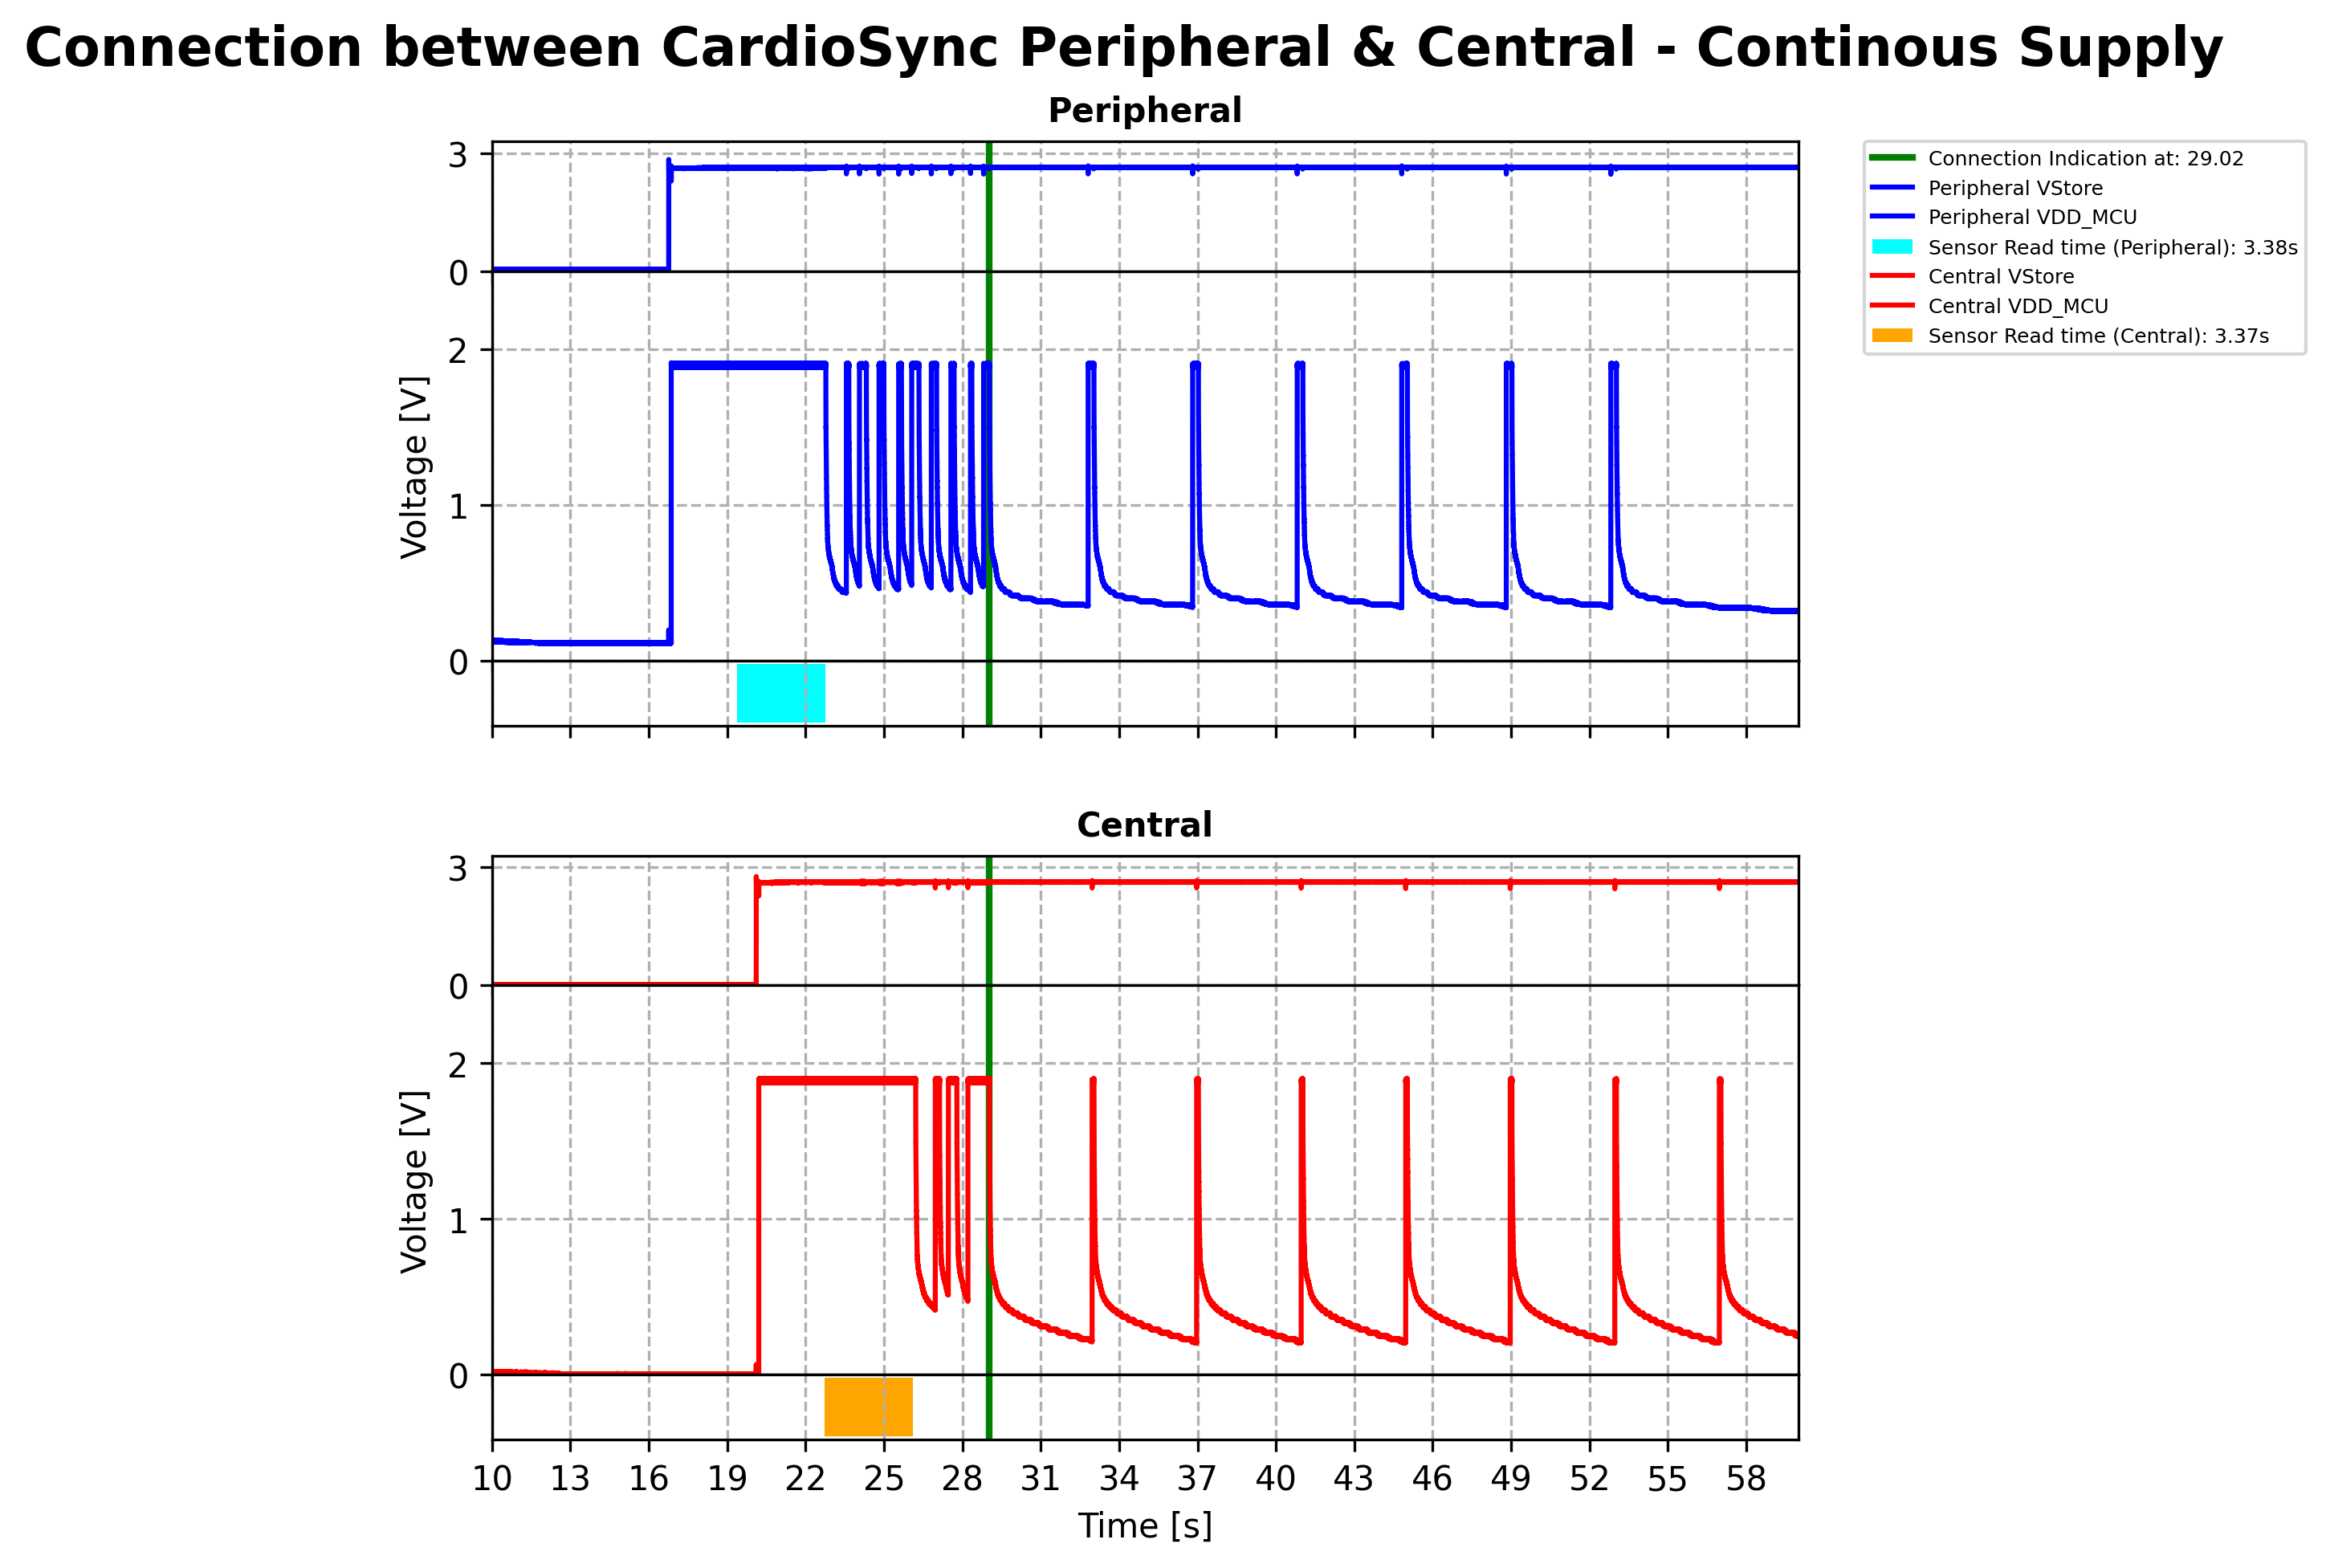
\includegraphics[width=0.95\linewidth]{chapters/Results/Connection_cardiosync_continous.png}
    \caption{Real-time Voltage measurement for the CardioSync system \textit{with Continuous supply} exhibiting a successful synchronised BLE connection}
    \label{fig:continous_connection_cardiosync}
\end{figure}

\begin{figure}[H]
    \centering
    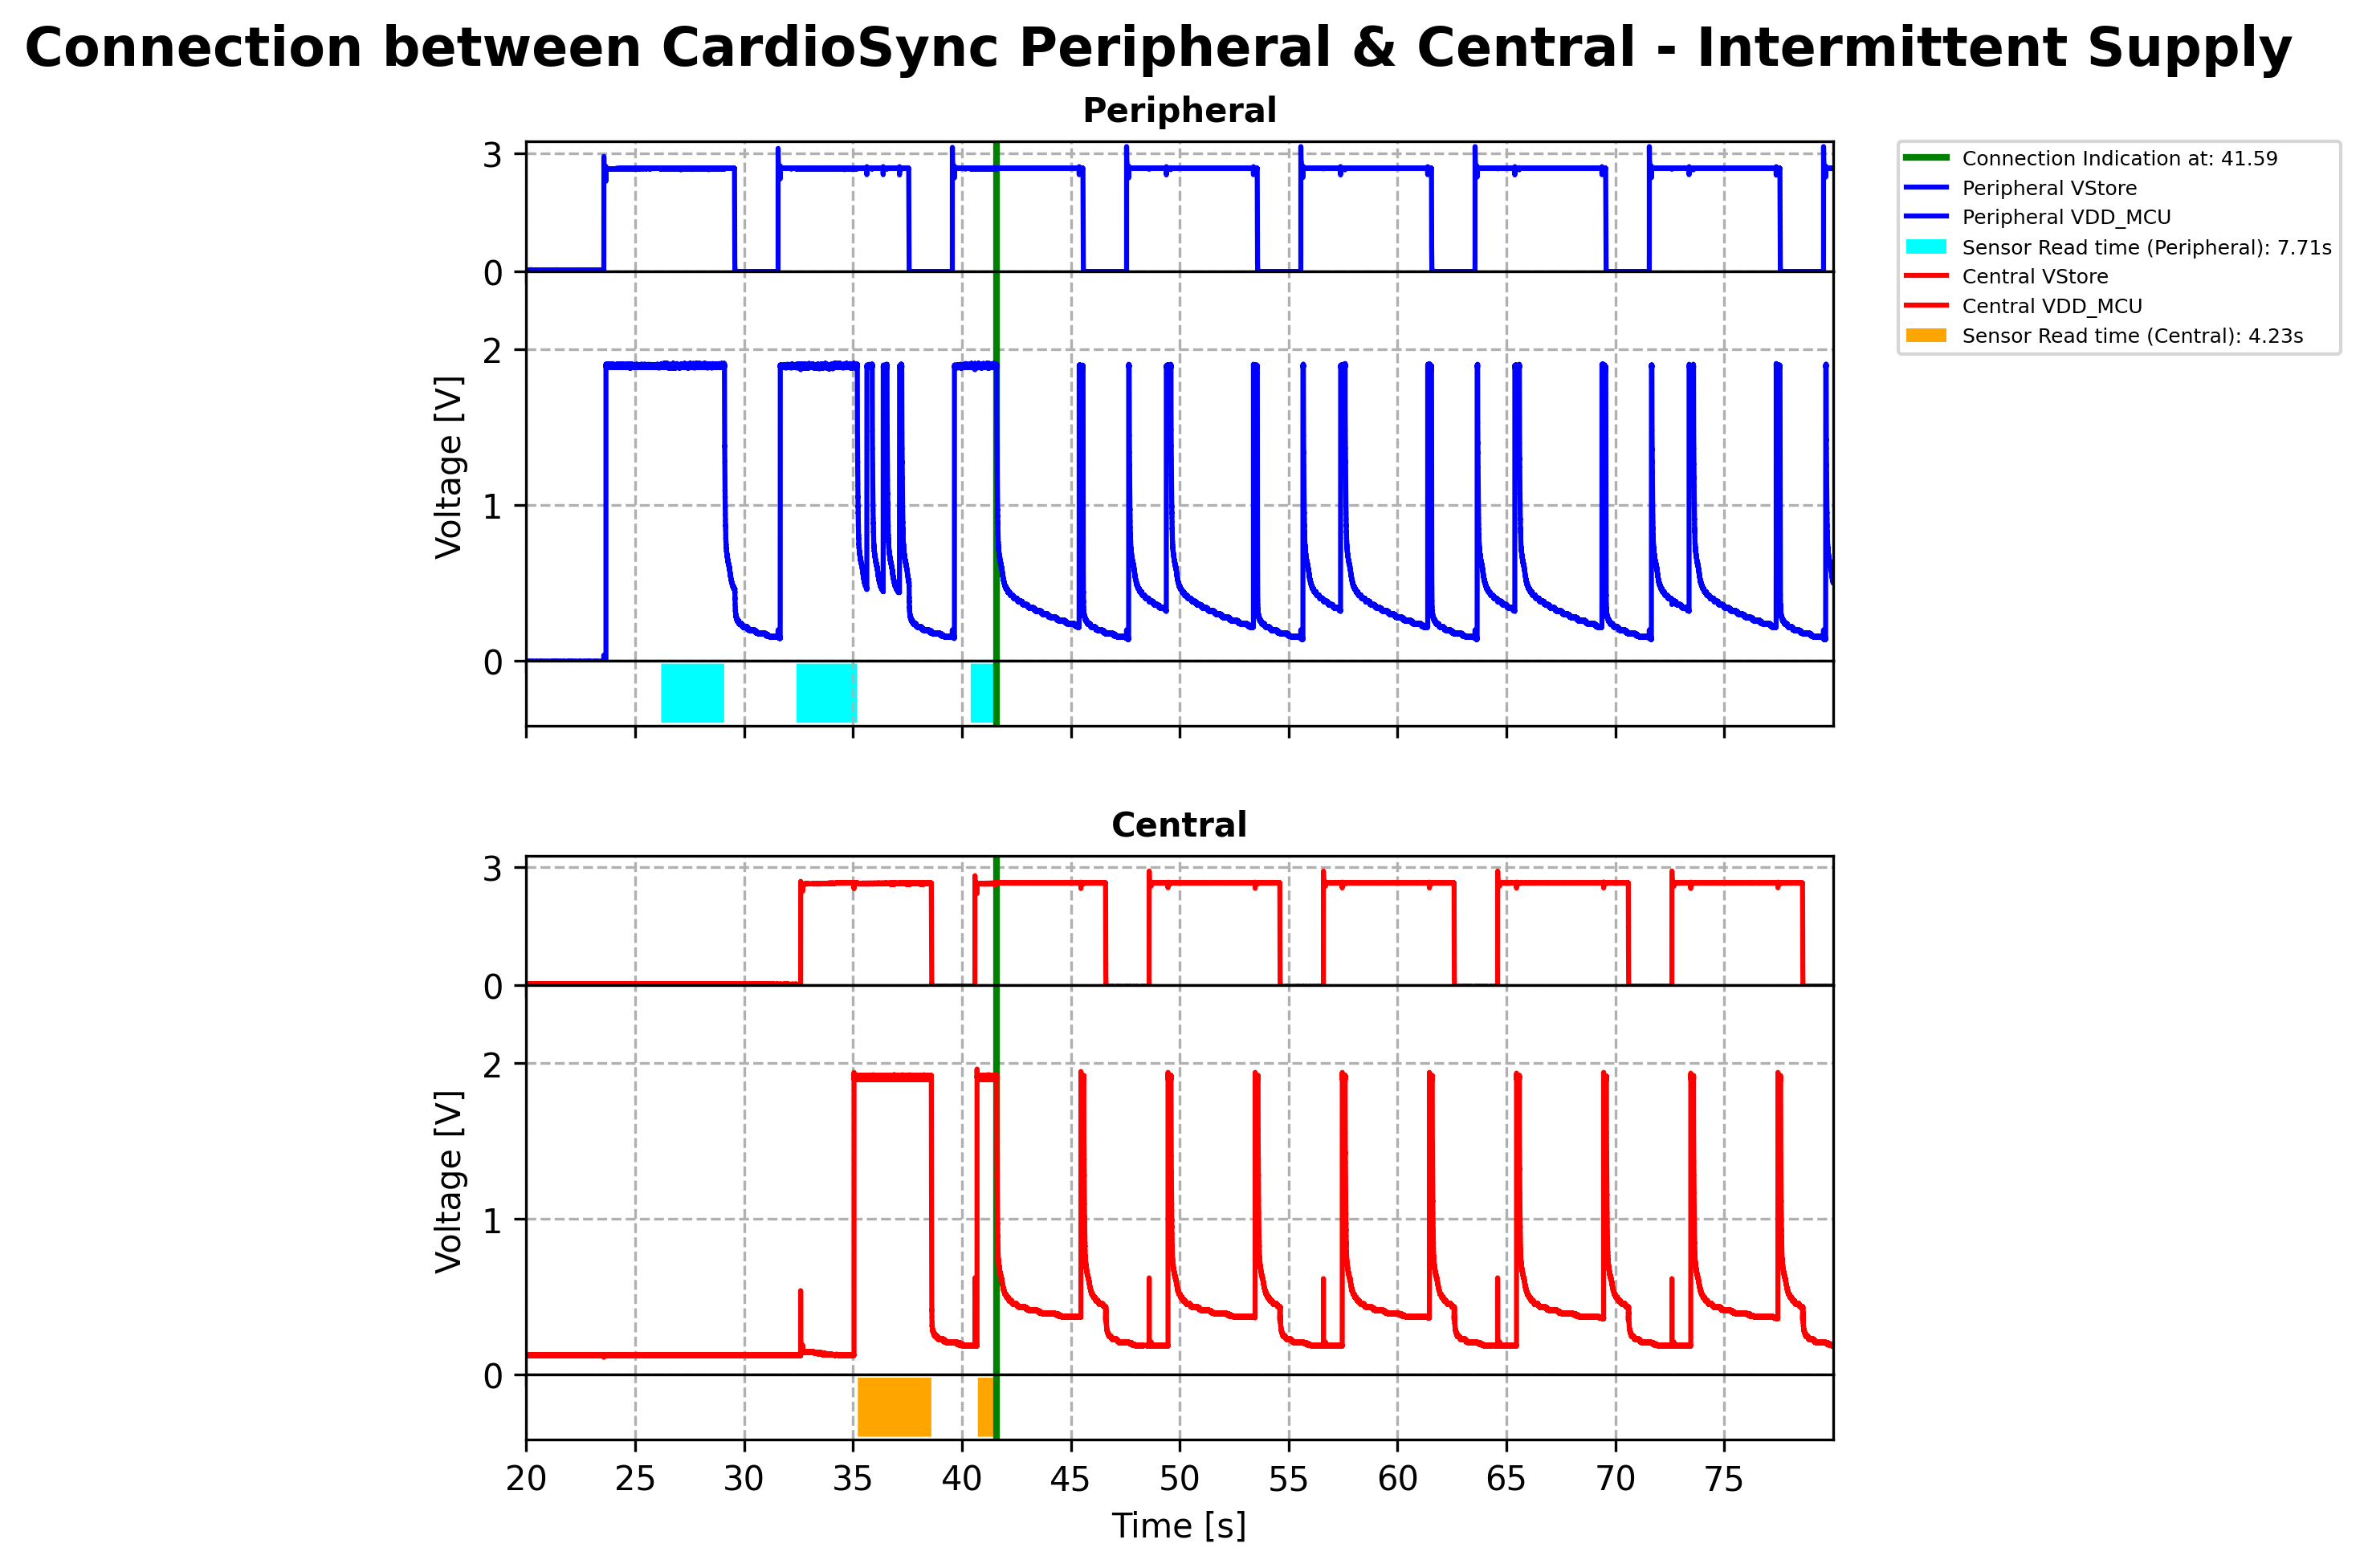
\includegraphics[width=0.95\linewidth]{chapters/Results/Connection_cardiosync_intermittent.png}
    \caption{Real-time Voltage measurement for the CardioSync system \textit{with Intermittent supply} exhibiting a successful synchronised BLE connection}
    \label{fig:intermittent_connection_cardiosync}
\end{figure}

\noindent The time series plots in \autoref{fig:current_cardiosync_central} and \autoref{fig:current_cardiosync_peripheral}, reveals the current measurement trend in real time for both central and peripheral's idle operation to read sensor and initiate BLE events based on heart rate peaks detected.

\begin{figure}[H]
    \centering
    \begin{subfigure}{0.85\linewidth}        
        \centering
        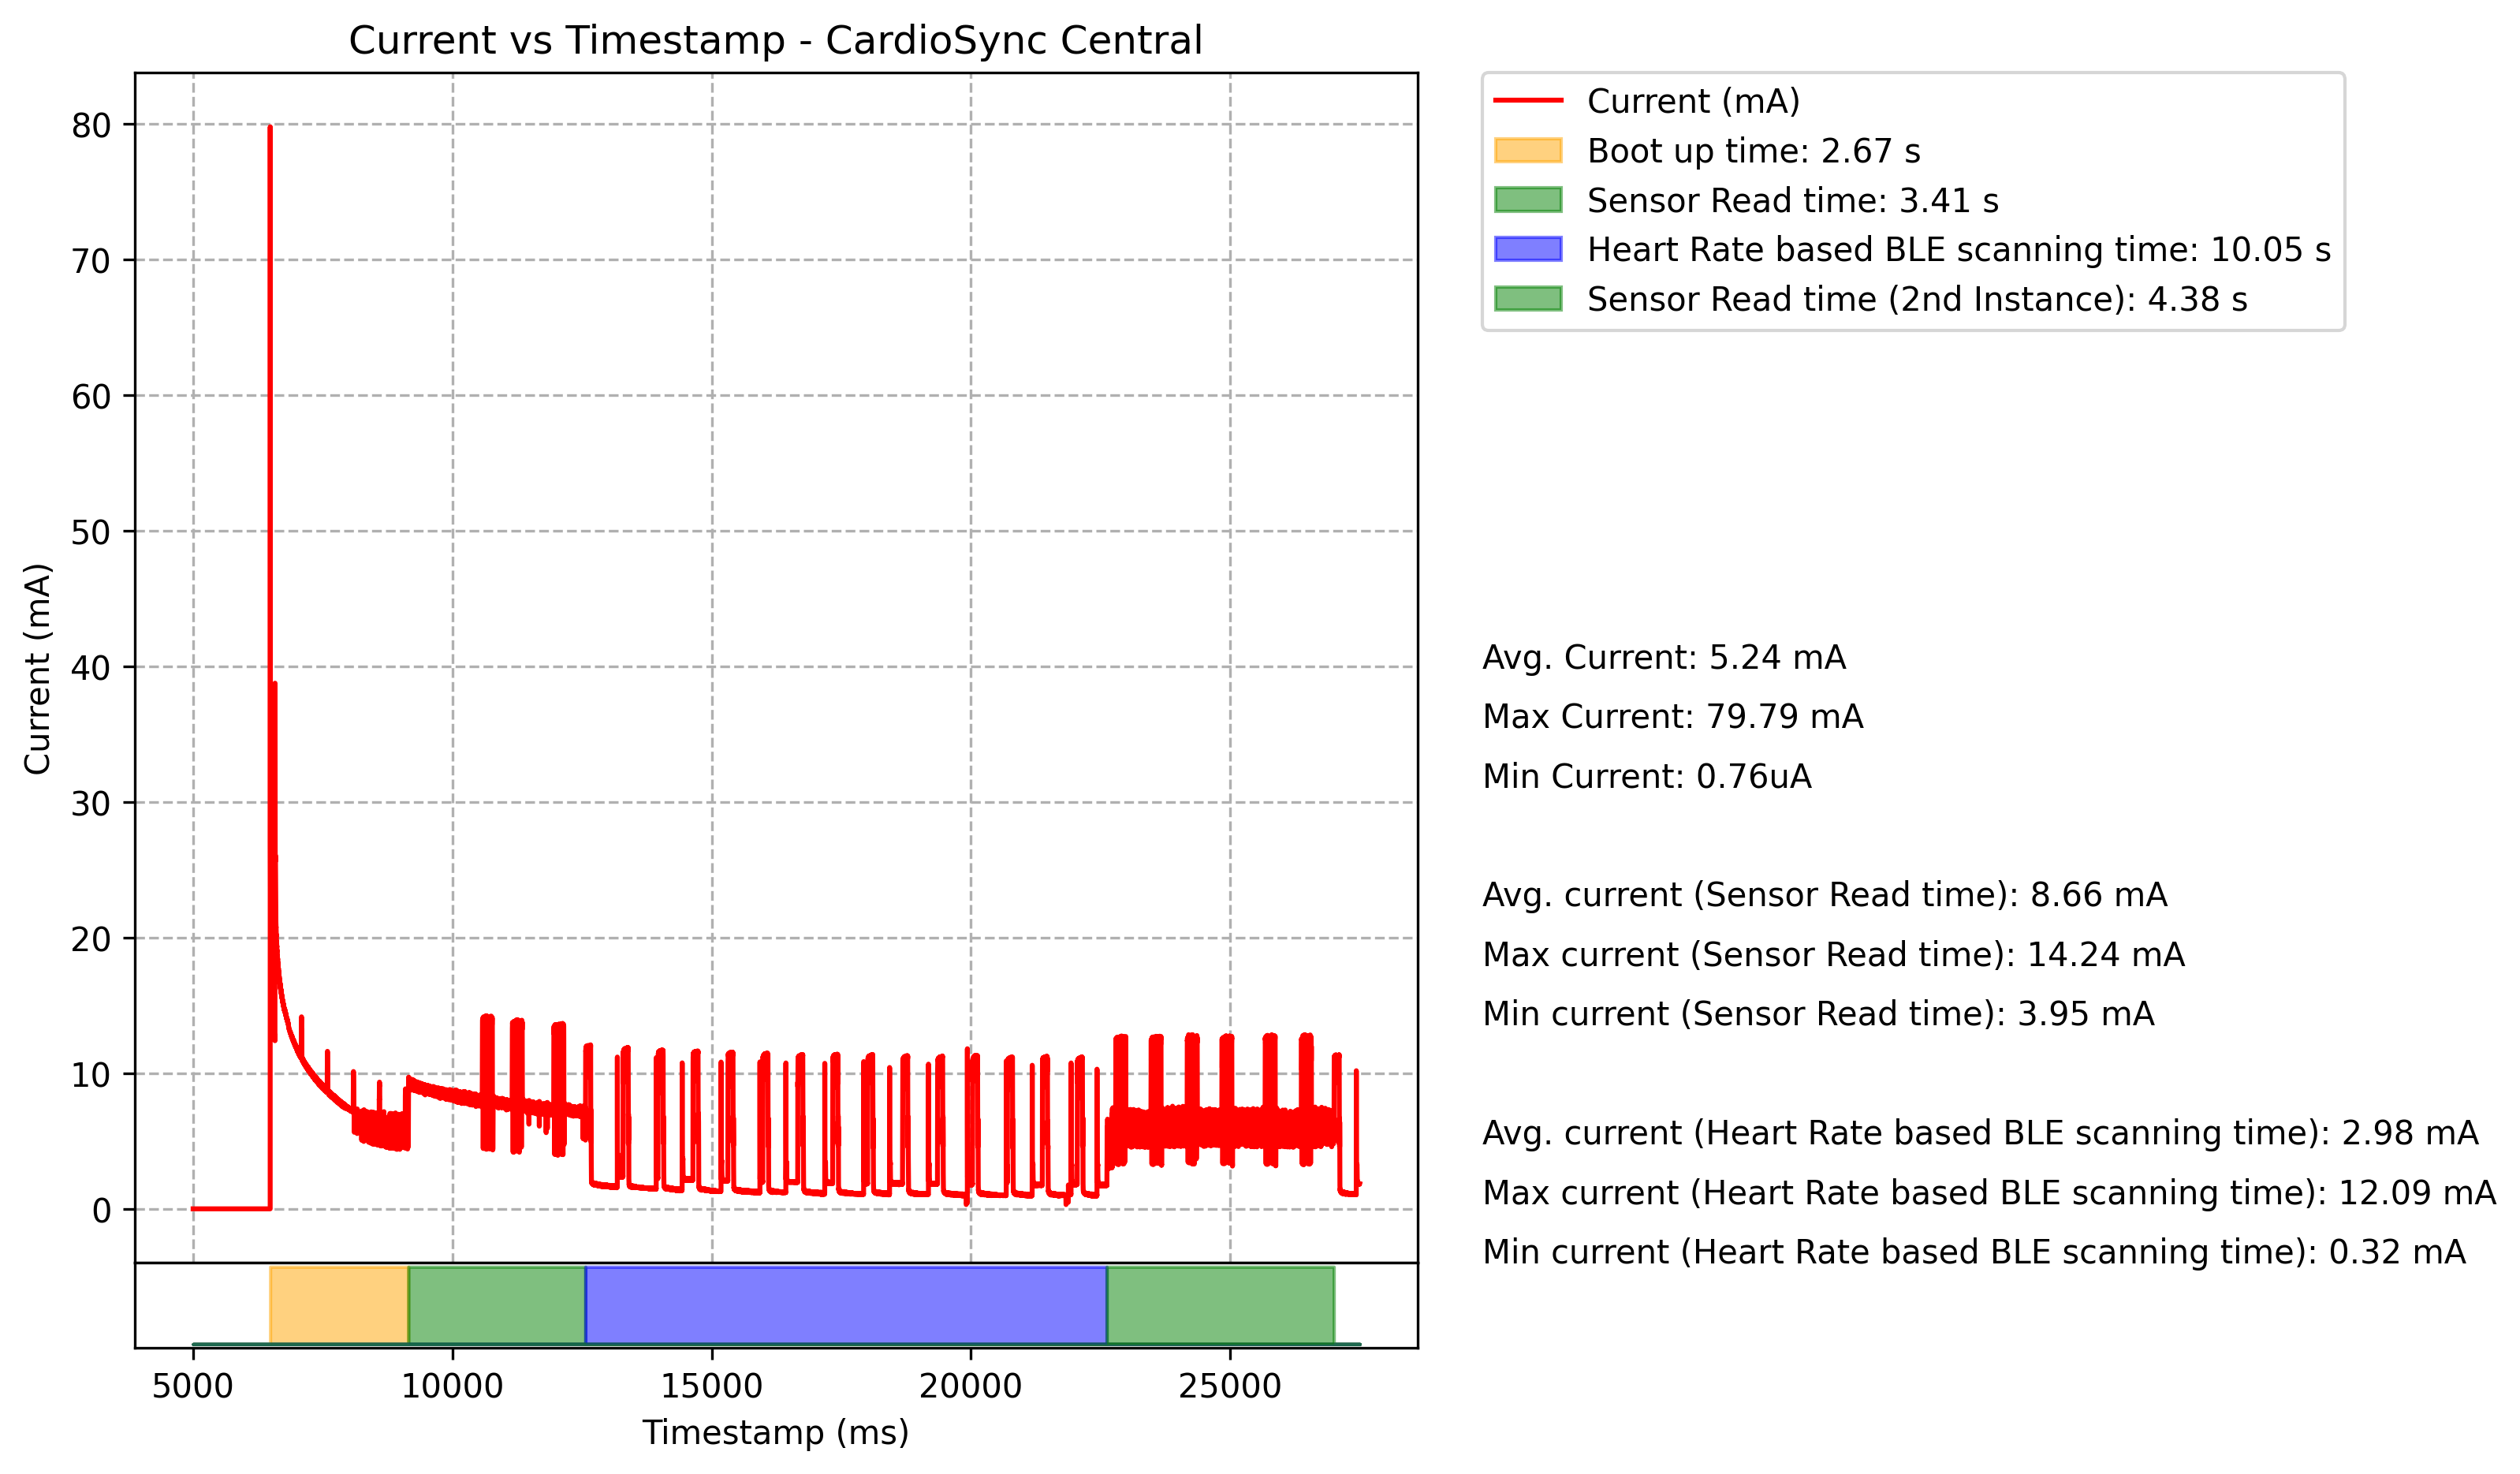
\includegraphics[width=\linewidth]{chapters/Results/Current vs Timestamp - CardioSync Central.png}
        \caption{Central}
        \label{fig:current_cardiosync_central}
    \end{subfigure}
    \begin{subfigure}{0.85\linewidth}    
        \centering
        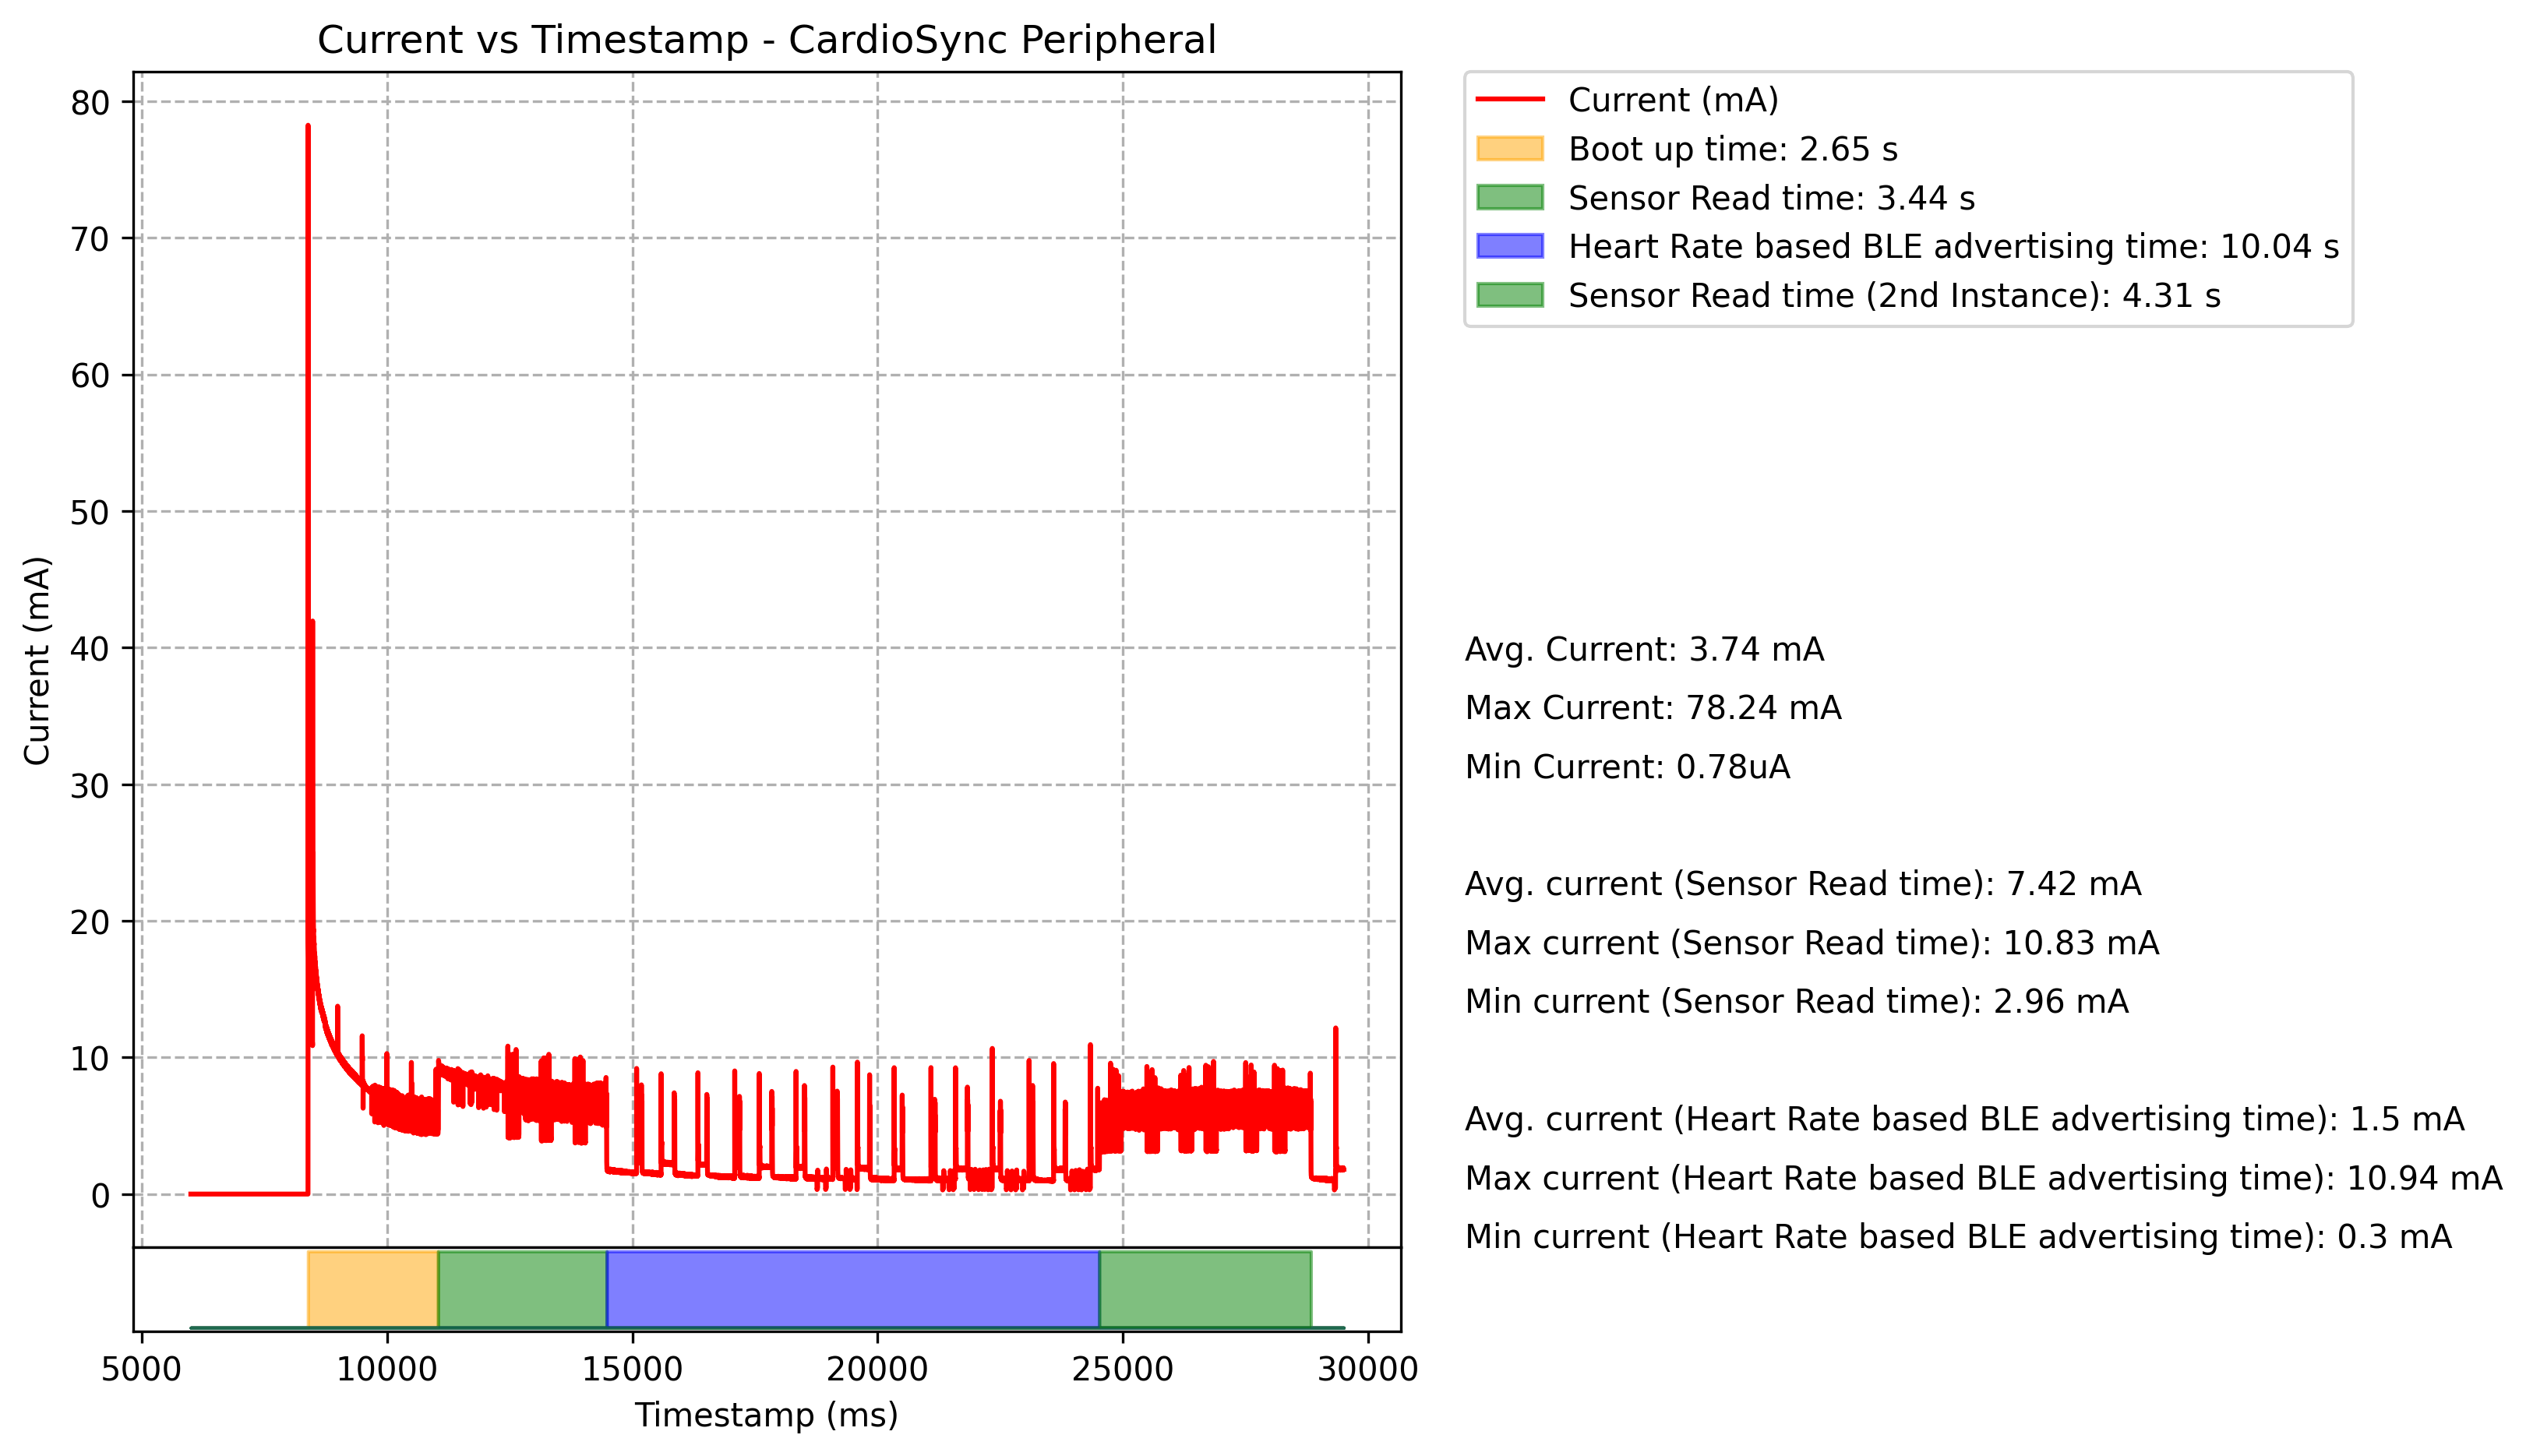
\includegraphics[width=\linewidth]{chapters/Results/Current vs Timestamp - CardioSync Peripheral.png}
        \caption{Peripheral}
        \label{fig:current_cardiosync_peripheral}
    \end{subfigure}
    \caption{Current measurement in Idle State without Connection establishment for CardioSync systems}
\end{figure}

\subsection{Interpretation of Results}

\subsubsection{Verification of system working in Continuous and Intermittent supply}
The time series plot depicted in \autoref{fig:continous_connection_cardiosync} illustrates the periodic shutdown of V\textsubscript{DD\_MCU} during times of inactivity, therefore corroborating the anticipated power-saving benefits associated with the integration of FreeBie. This finding provides evidence for the effectiveness of incorporating a sensor into a batteryless system. 

\noindent The first period following the startup of the CardioSync system involves the central and peripheral devices engaging in the process of reading the sensor data and determining the present heart rate. This can be observed from the plot, which indicates that the devices spend around \textit{3.40 seconds} for this task. As elucidated in Chapter 3, the system demonstrates the anticipated functionality of power saving after the initial sensor reading. That can noted from the plot too as the device enters a dormant state and exclusively reactivates at the interval of each heartbeat pulse in order to initiate a Bluetooth Low Energy (BLE) connection. The connection establishment event, which is closely synced with the heart rate pulses, is shown by the green vertical line in plot \ref{fig:continous_connection_cardiosync}.

\noindent Once the connection is established, we could see the V\textsubscript{DD\_MCU} turning off and resumes only when there is a BLE event. During this period, we don't see sensor getting activated or read, that can be confirmed from plot as well as GPIO pins indicating sensor read was low.

\noindent A similar verification was conducted under intermittent power supply conditions using a square wave signal with a duty cycle of 75\% for a duration of 8 seconds. The time series plot (\autoref{fig:intermittent_connection_cardiosync}) reveals the system's adaptability to changing power availability, as connections continue to be established in coordination with the heart beat, despite power fluctuations. In addition, the CardioSync system was tested across various square wave periods with different duty cycles, demonstrating its adaptability to different supply configurations. Notably, the data underscored the system's superior performance with lower turn-off periods, a characteristic that aligns with the inherent strengths of the FreeBie framework.

\subsubsection{Current Measurement of CardioSync system}
The \autoref{fig:current_cardiosync_central} and \autoref{fig:current_cardiosync_peripheral}, gives us the current reading for different phases of the CardioSync system operation for synchronising BLE connection.

\noindent It is important to note that the sensor read phase requires a higher current compared to the heart rate based dormant phase. This is because in sensor read phase, the microcontroller is actively engaged in reading the sensor at a sample rate of 100Hz in order to detect the heart rate peaks and calculate the heart rate interval. Upon determination of heart rate interval, it becomes evident that the average current experiences a significant reduction since the device only activates during each heart pulse interval for the purpose of BLE advertising or scanning.

\noindent This behavior is substantiated across both central and peripheral devices in the current measurement-driven evaluation. In the Central device, active sensor reading for \textit{3.41 seconds} consumes an average current of approximately \textit{8.66mA}, while the Peripheral device registers \textit{7.42mA} over a \textit{3.44-second} interval. Notably, during the heart rate-dependent sleep phase of longer 10 seconds, both central and peripheral devices exhibit a substantially lower average current consumption—\textit{2.98mA and 1.5mA}, respectively. The device's activation solely during heart pulse intervals for BLE advertising or scanning culminates in a notable reduction in overall average current.

\noindent The values of these evaluation are afterwards utilized in the computation of the energy expended by the device for the purpose of synchronizing a BLE connection, which will be further analyzed in the subsequent section for comparison.

\section{Comparative Analysis against Reference Design:}
Having thoroughly evaluated the heart rate sensor's algorithm and its successful integration into the existing FreeBie battery-free BLE framework, our exploration up to this juncture has yielded compelling results that affirm the system's intended functionality. In this section, we start with our attention towards introducing a reference model of Battery-Free BLE. This model will be used as a yardstick to gauge the effectiveness of our synchronized BLE system. Through this comparative lens, we not only underscore the strengths and merits of our CardioSync system, elucidating its capability in enhancing connectivity and efficiency within battery-free environments, but also keenly uncover any potential shortcomings.

\subsection{Reference FreeBie model}
To provide a more comprehensive comparison, the reference system used is the Freebie system, which does not employ any synchronization method. FreeBie employs a strategy of establishing a Bluetooth Low Energy (BLE) connection by using periodic advertising and scanning techniques. However, a drawback of the periodic attempt to establish a connection depends on the potential scenario where central and peripheral devices fail to coordinate their sleep and waking cycles, hence resulting in the possibility of a permanent failure to establish a link between them. For experimental reasons, the Central and Peripheral components of the FreeBie reference model were activated with intentionally matched Advertising and Scanning intervals. 

\noindent To have more data points for comparison, three different BLE configurations of FreeBie is chosen that has different energy consumption and it is outlined in  the \autoref{tab:ble_params_freebie}.

\begin{table}[H]
\centering
\begin{tabular}{|c|cc|}
\hline
\textbf{\begin{tabular}[c]{@{}c@{}}Configuration\\ Name\end{tabular}} & \multicolumn{2}{c|}{\textbf{\begin{tabular}[c]{@{}c@{}}Configured BLE\\ parameters\end{tabular}}} \\ \hline
\cellcolor[HTML]{32CB00} & \multicolumn{1}{c|}{\textit{\begin{tabular}[c]{@{}c@{}}Advertising\\ Interval\end{tabular}}} & 6 seconds        \\ \cline{2-3} 
\cellcolor[HTML]{32CB00} & \multicolumn{1}{c|}{\textit{\begin{tabular}[c]{@{}c@{}}Scanning\\ Interval\end{tabular}}}    & 6 seconds        \\ \cline{2-3} 
\multirow{-3}{*}{\cellcolor[HTML]{32CB00}\textbf{Low}}    & \multicolumn{1}{c|}{\textit{\begin{tabular}[c]{@{}c@{}}Scanning\\ Window\end{tabular}}} & 1 second         \\ \hline
\cellcolor[HTML]{FFCB2F} & \multicolumn{1}{c|}{\textit{\begin{tabular}[c]{@{}c@{}}Advertising\\ Interval\end{tabular}}} & 2 seconds        \\ \cline{2-3} 
\cellcolor[HTML]{FFCB2F} & \multicolumn{1}{c|}{\textit{\begin{tabular}[c]{@{}c@{}}Scanning\\ Interval\end{tabular}}}    & 2 seconds        \\ \cline{2-3} 
\multirow{-3}{*}{\cellcolor[HTML]{FFCB2F}\textbf{Medium}} & \multicolumn{1}{c|}{\textit{\begin{tabular}[c]{@{}c@{}}Scanning\\ Window\end{tabular}}} & 500 milliseconds \\ \hline
\cellcolor[HTML]{FD6864} & \multicolumn{1}{c|}{\textit{\begin{tabular}[c]{@{}c@{}}Advertising\\ Interval\end{tabular}}} & 500 milliseconds \\ \cline{2-3} 
\cellcolor[HTML]{FD6864} & \multicolumn{1}{c|}{\textit{\begin{tabular}[c]{@{}c@{}}Scanning\\ Interval\end{tabular}}}    & 500 milliseconds \\ \cline{2-3} 
\multirow{-3}{*}{\cellcolor[HTML]{FD6864}\textbf{High}}   & \multicolumn{1}{c|}{\textit{\begin{tabular}[c]{@{}c@{}}Scanning\\ Window\end{tabular}}} & 125 milliseconds \\ \hline
\end{tabular}
\caption{Chosen BLE parameters for Reference FreeBie system}
\label{tab:ble_params_freebie}
\end{table}


\noindent Investigating the Reference Freebie system under varying energy configurations, three distinct scenarios were examined: low, medium, and high energy. Time series plots were generated for each configuration using the same experimental setup discussed in section \ref{sec:experimental_setup} and are presented as Plots in Figures \ref{fig:freebie_low_conn}, \ref{fig:freebie_medium_conn} and \ref{fig:freebie_high_conn}, respectively. These plots capture connection establishment in response to periodic BLE events. It is also evident that during the intervals between these events, the device enters a sleep state, as shown by the V\textsubscript{DD\_MCU} plot on both the Central and Peripheral sides.

\noindent Also, additionally the current trend during idle time of the FreeBie system for each BLE parameters configuration can be seen in \autoref{fig:freebie_low_central}, \autoref{fig:freebie_low_peripheral}, \autoref{fig:freebie_medium_central}, \autoref{fig:freebie_medium_peripheral}, \autoref{fig:freebie_high_central} and \autoref{fig:freebie_high_peripheral}.The average current needed by the system during attempts to establish a Bluetooth Low Energy (BLE) connection under various Scan and Advertisement configurations was measured. This data was then used for comparative analysis of energy and power.

\begin{table}[H]
\centering
\begin{tabular}{|c|cc|}
\hline
 &
  \multicolumn{2}{c|}{\textit{\textbf{\begin{tabular}[c]{@{}c@{}}Average Current measured\\ in mA\end{tabular}}}} \\ \cline{2-3} 
\multirow{-2}{*}{\textit{\textbf{\begin{tabular}[c]{@{}c@{}}Configuration\\ Name\end{tabular}}}} &
  \multicolumn{1}{c|}{\textit{\textbf{Central}}} &
  \textit{\textbf{Peripheral}} \\ \hline
\cellcolor[HTML]{32CB00}Low    & \multicolumn{1}{c|}{\textit{1.77}} & 0.07 \\ \hline
\cellcolor[HTML]{FFCB2F}Medium & \multicolumn{1}{c|}{\textit{2.78}} & 0.16 \\ \hline
\cellcolor[HTML]{FD6864}High   & \multicolumn{1}{c|}{\textit{2.85}} & 0.6  \\ \hline
\end{tabular}
\caption{Average current reading for each of the reference system configuration.}
\label{tab:avg_current_freebie}
\end{table}
\begin{figure}[H]
    \begin{subfigure}{0.5\linewidth}
        \centering
        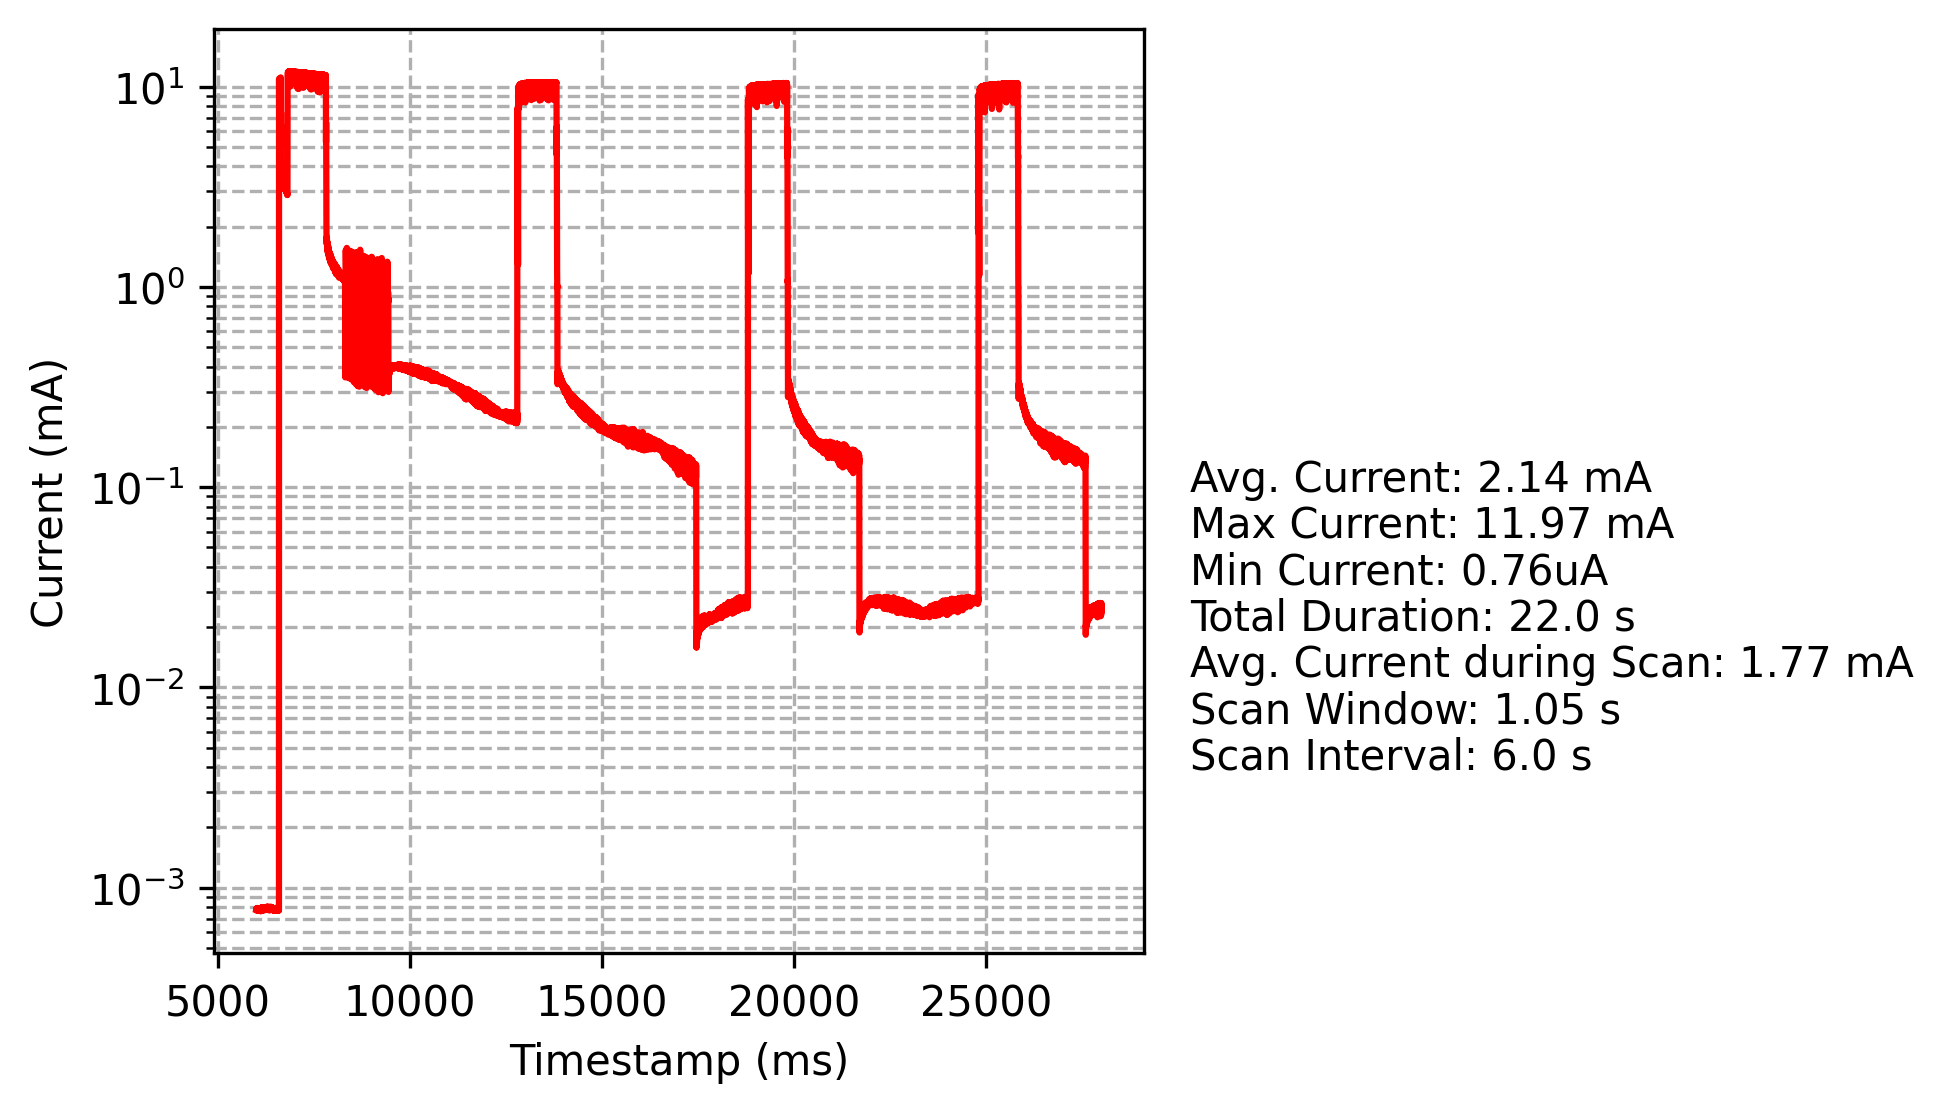
\includegraphics[width=0.8\linewidth]{chapters/Results/Current vs Timestamp - FreeBie Central Low.png}
        \caption{Current Measurement in Idle State - Central}
        \label{fig:freebie_low_central}
    \end{subfigure}
    \begin{subfigure}{0.5\linewidth}
        \centering
        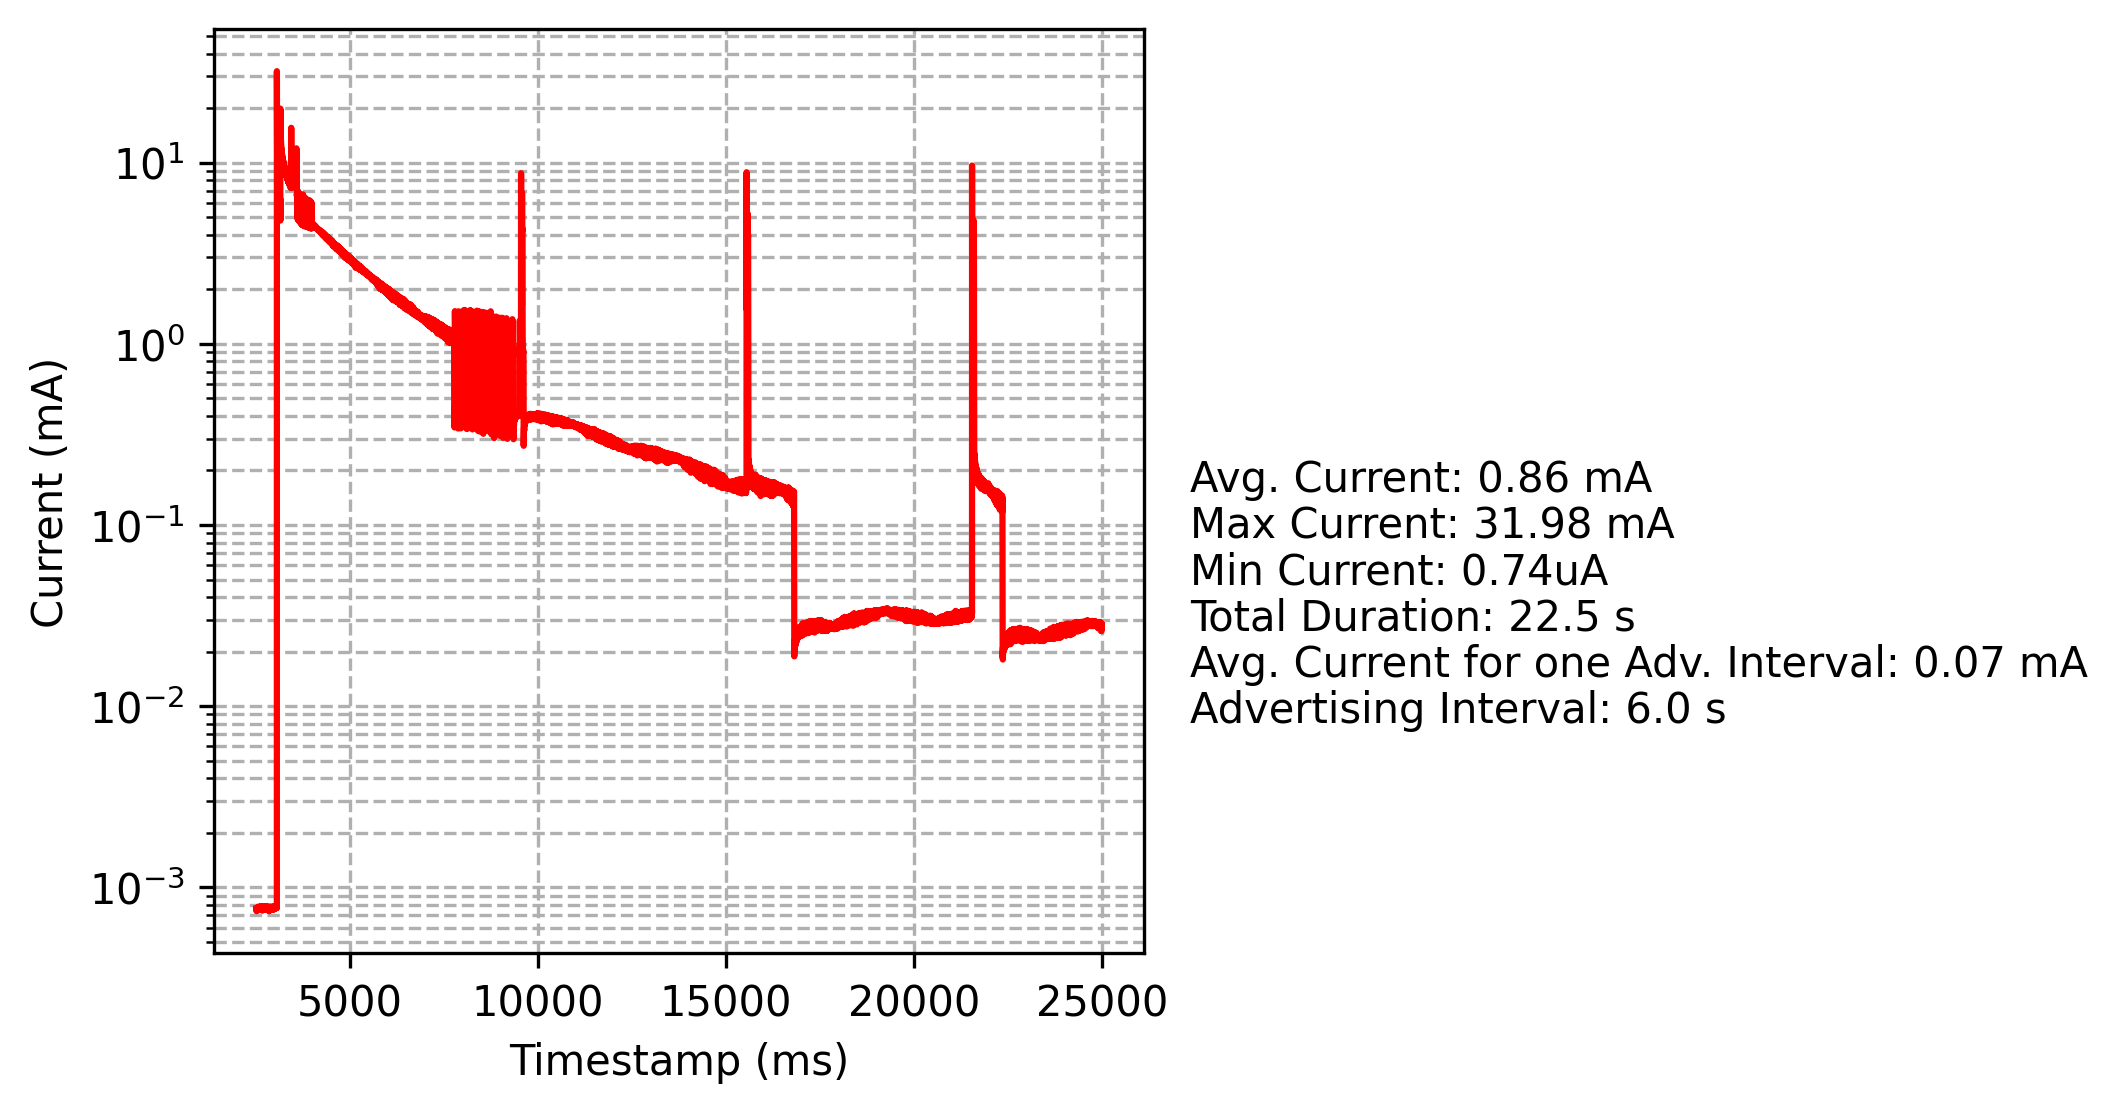
\includegraphics[width=0.8\linewidth]{chapters/Results/Current vs Timestamp - FreeBie Peripheral Low.png}
        \caption{Current Measurement in Idle State - Peripheral}
        \label{fig:freebie_low_peripheral}
    \end{subfigure}
    \begin{center}
        \begin{subfigure}{0.5\linewidth}
            \centering
            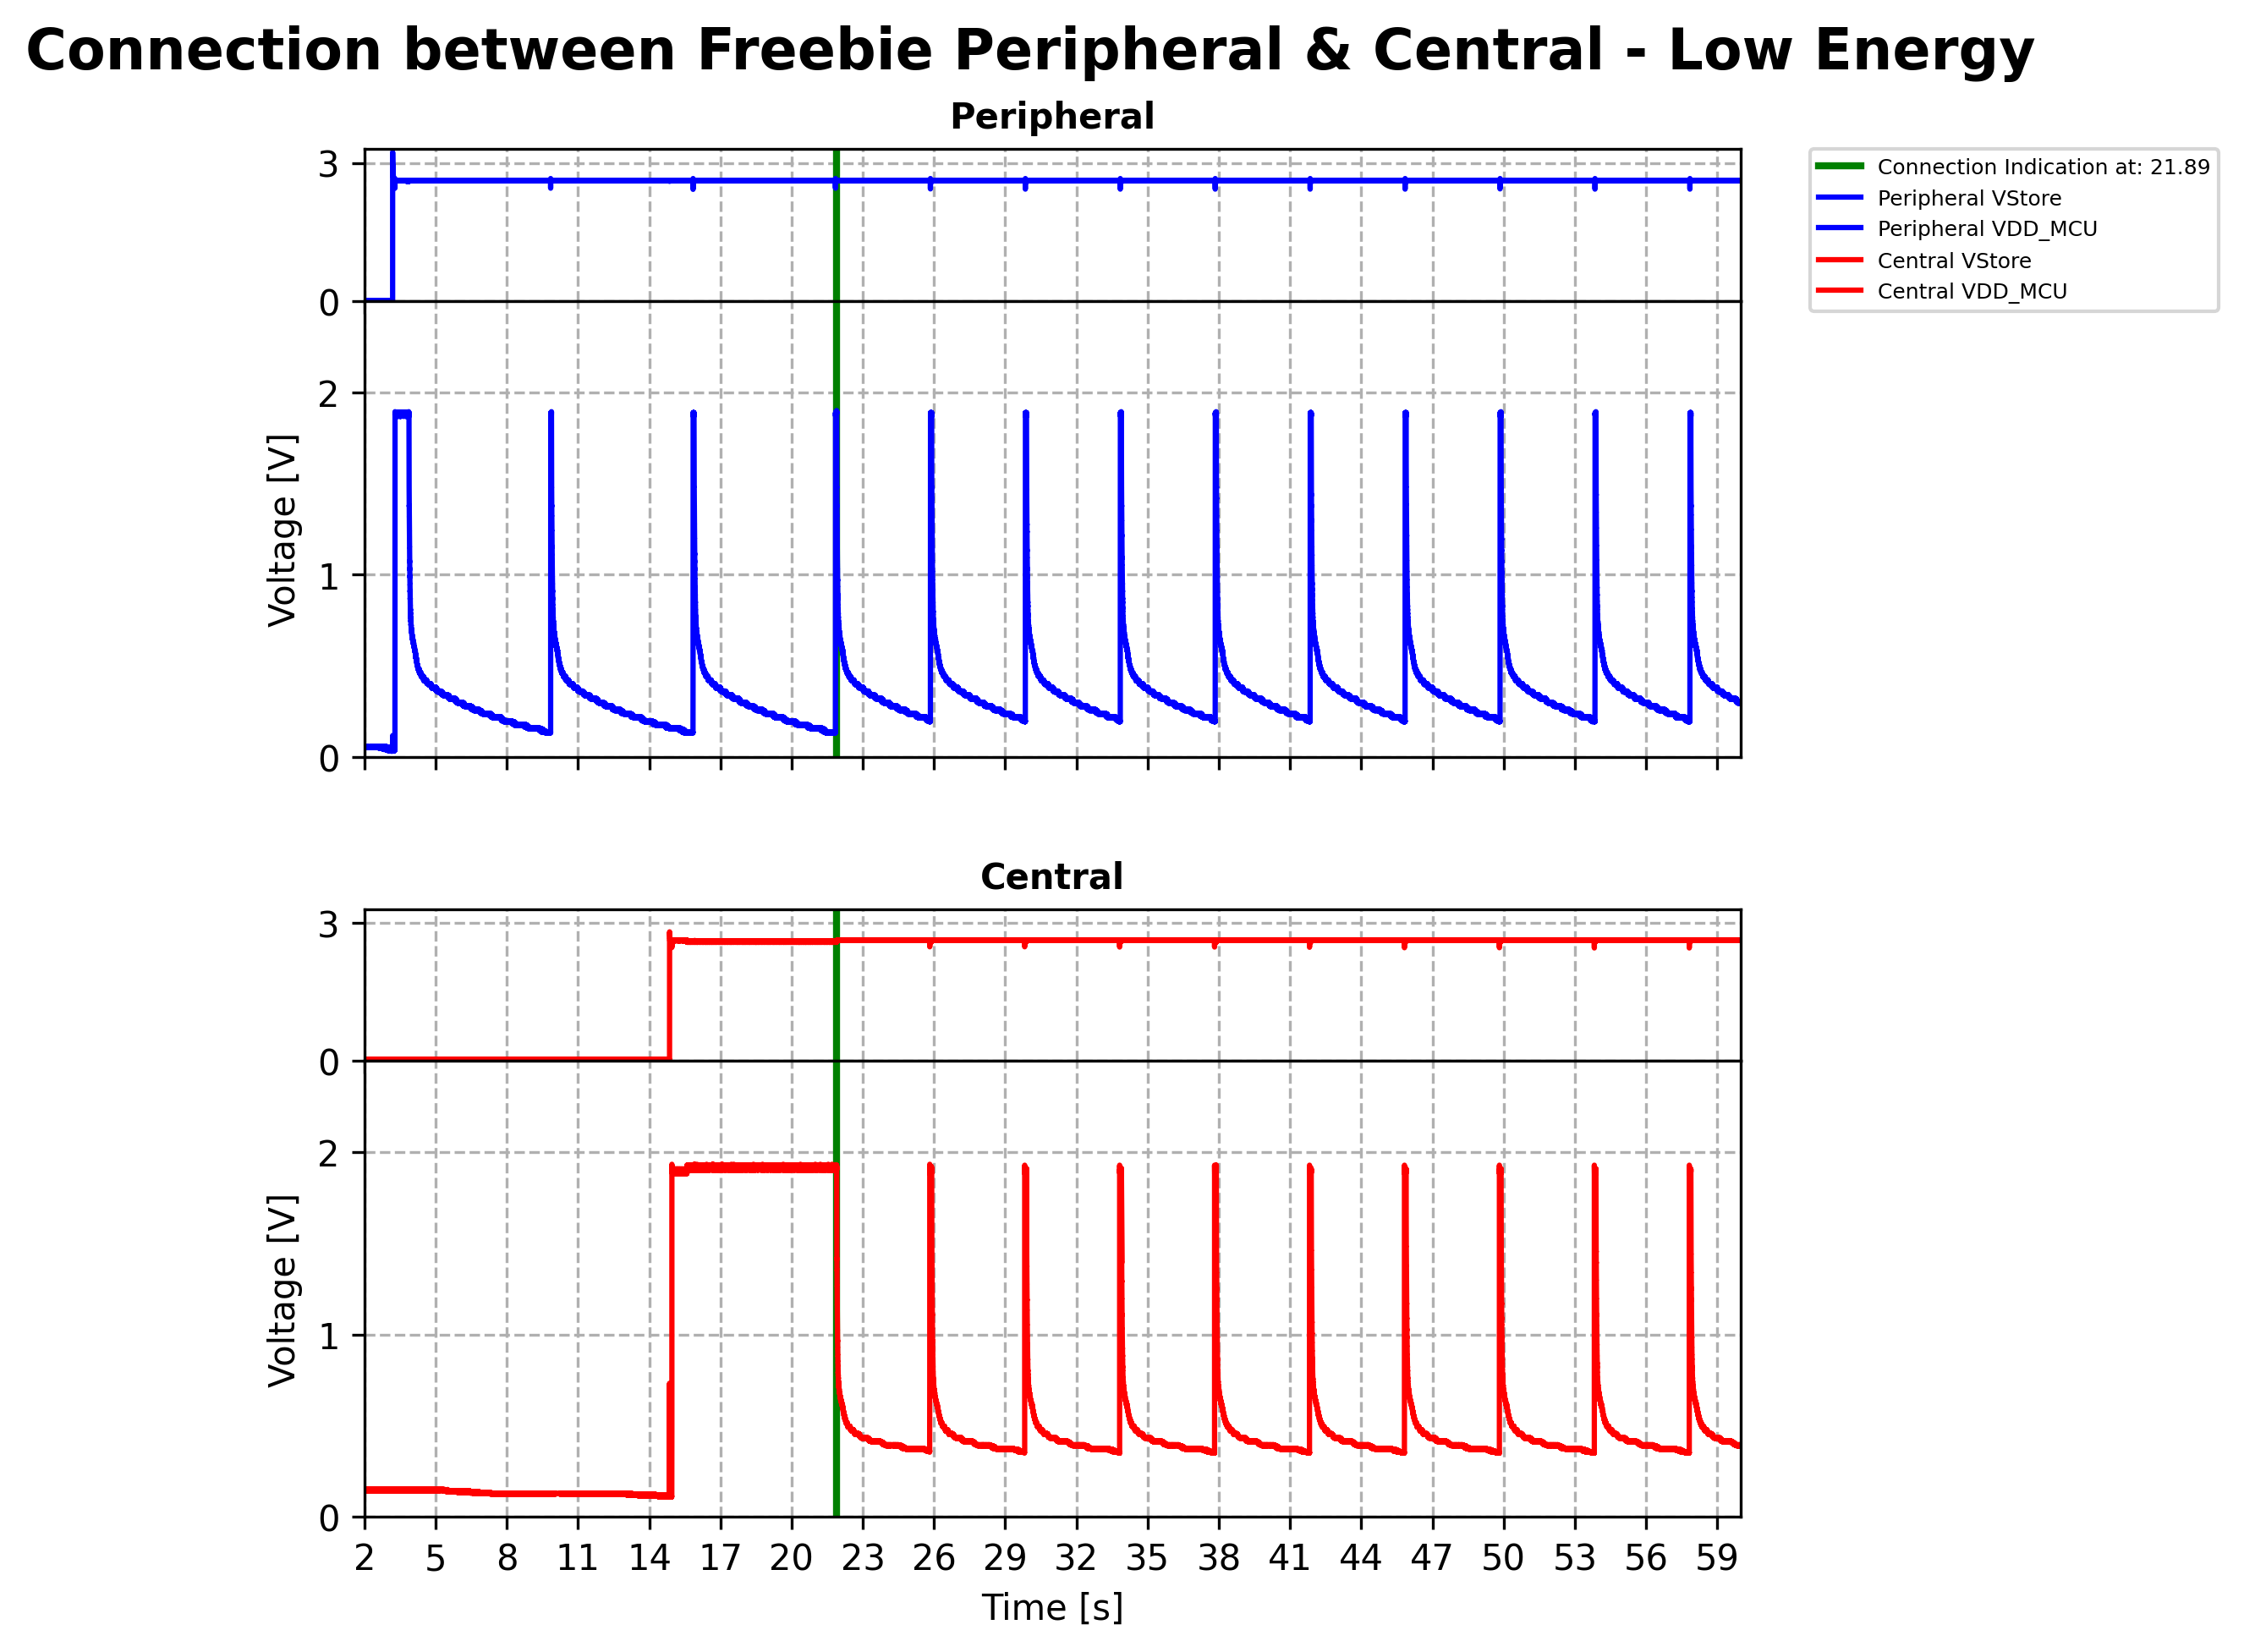
\includegraphics[width=\linewidth]{chapters/Results/Connection_Freebie_low.png}
            \caption{Voltage Measurement trend exhibiting a successful BLE connection}
            \label{fig:freebie_low_conn}
        \end{subfigure}    
    \end{center}
    \caption{\centering Time series plots showing behavior of FreeBie Low system}
\end{figure}
\begin{figure}[H]
    \begin{subfigure}{0.5\linewidth}
        \centering
        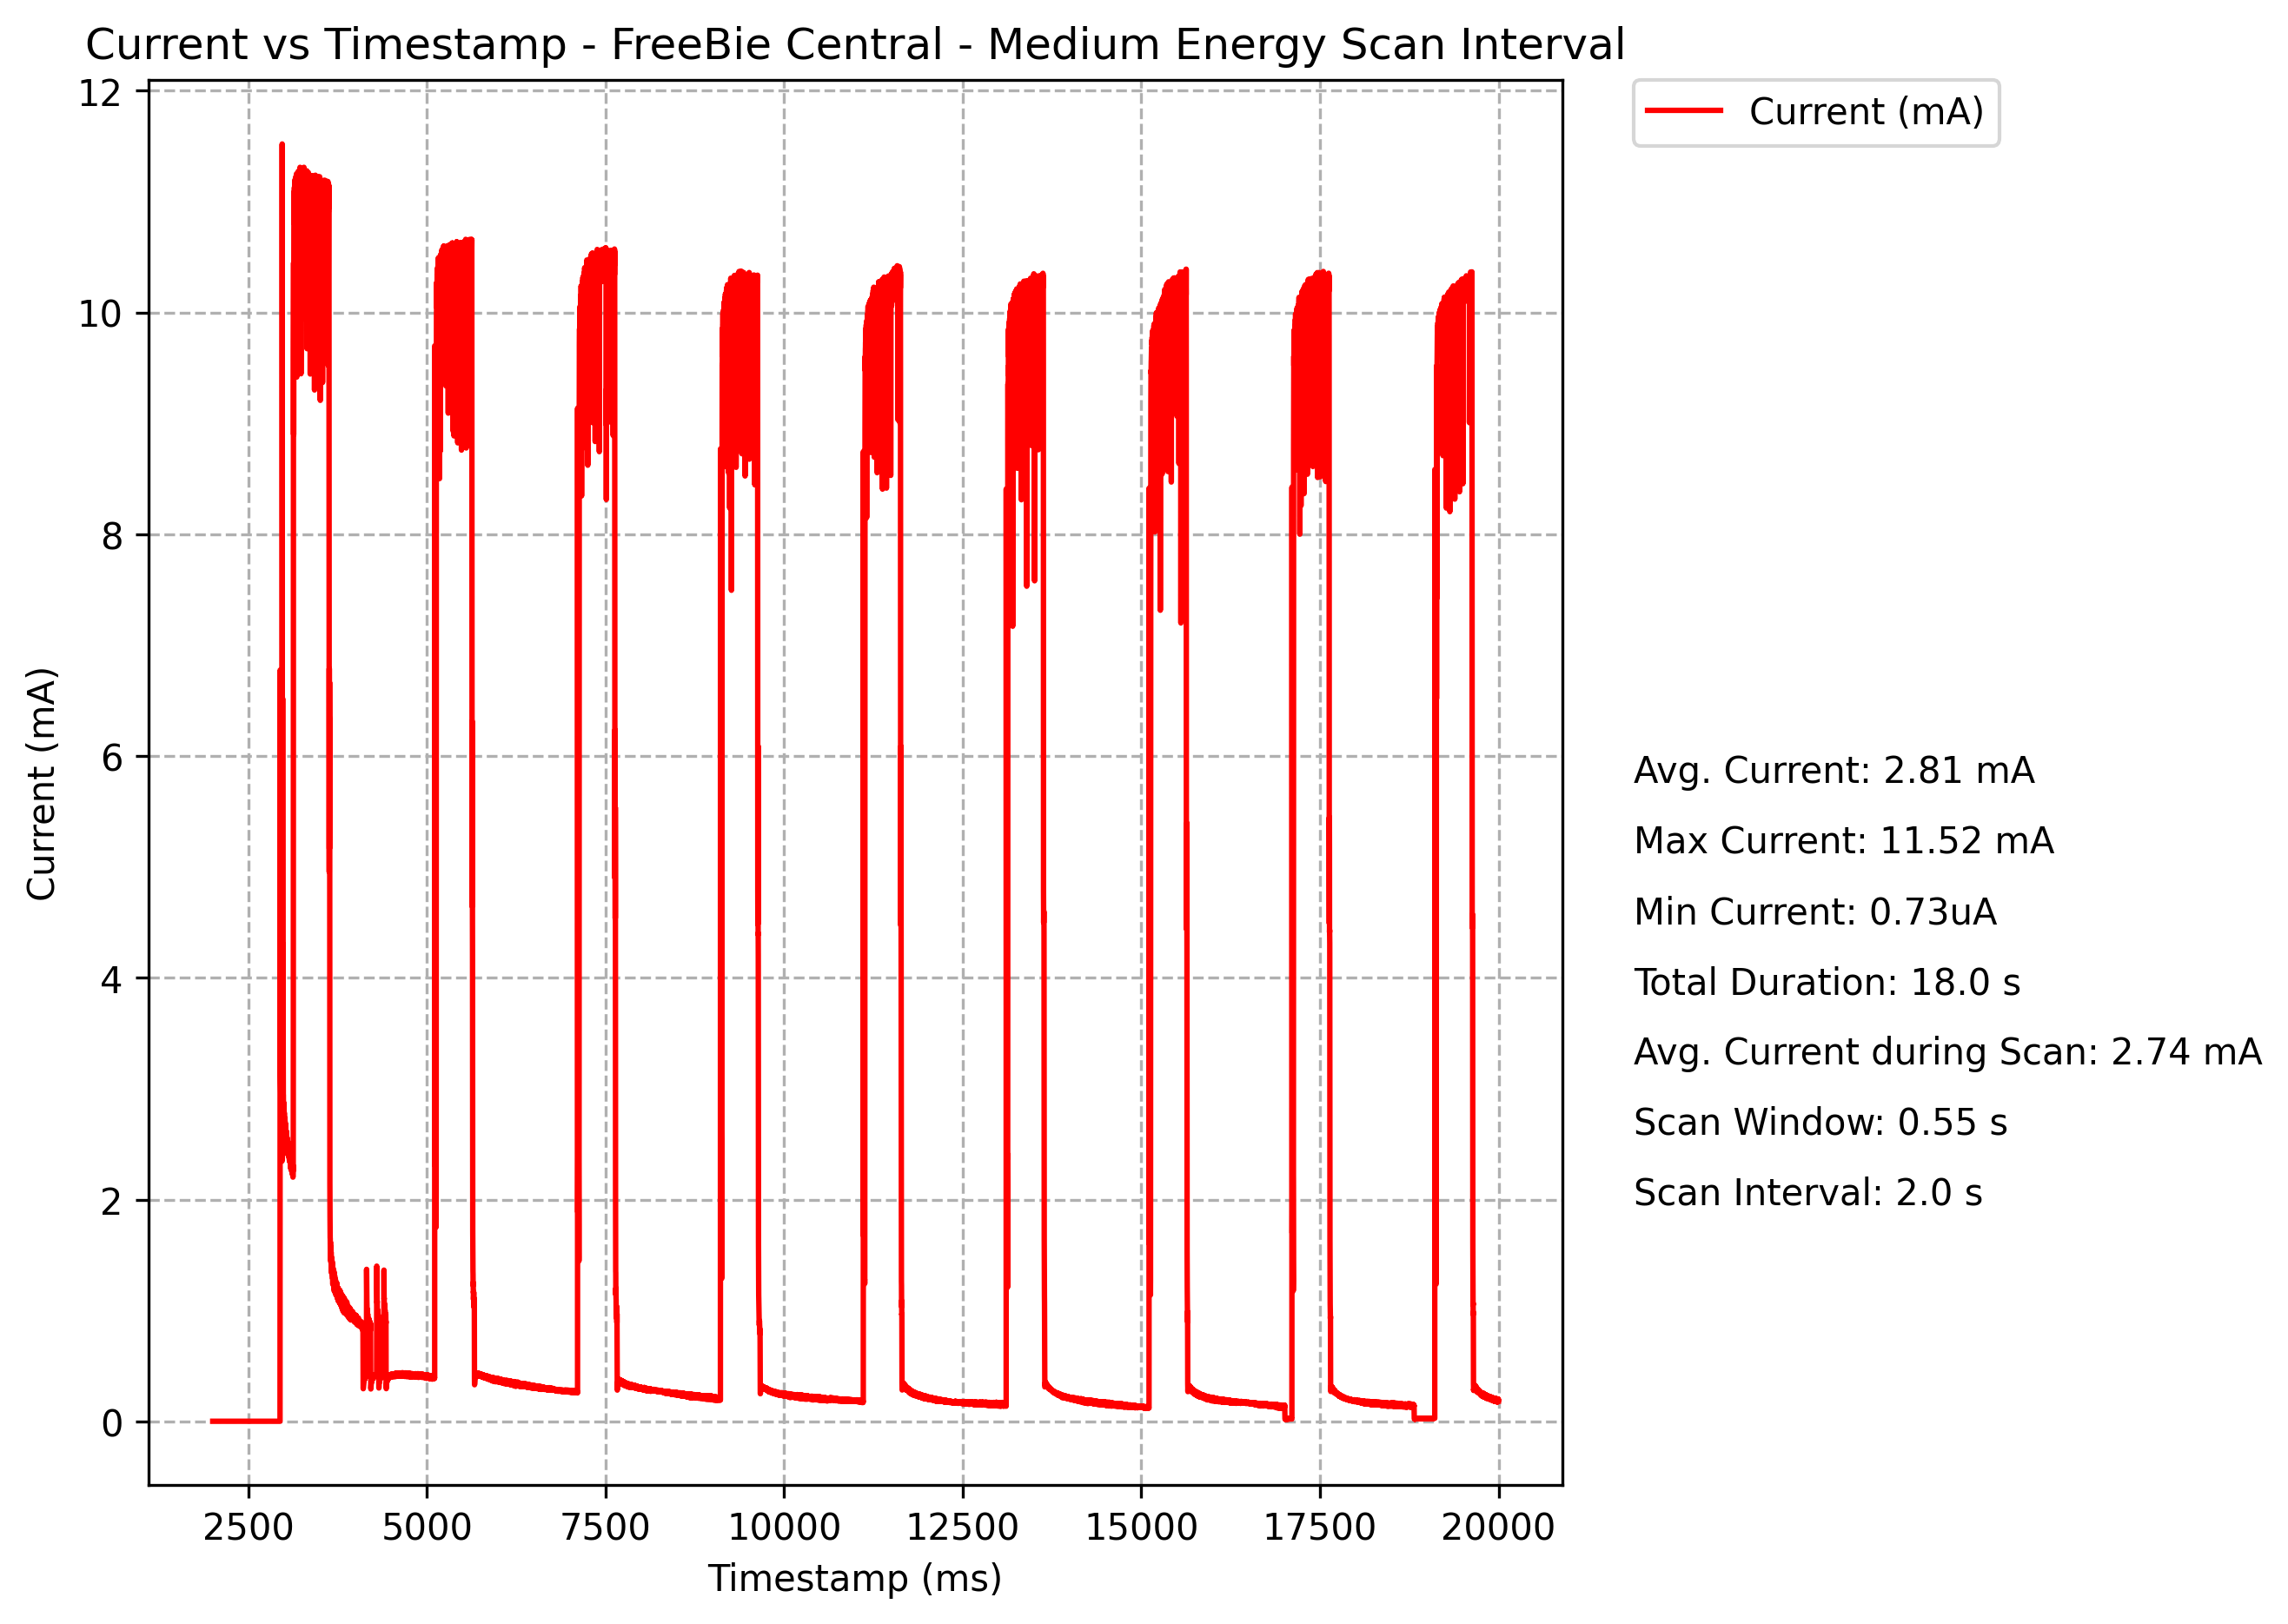
\includegraphics[width=0.8\linewidth]{chapters/Results/Current vs Timestamp - FreeBie Central Medium.png}
        \caption{Current Measurement in Idle State - Central}
        \label{fig:freebie_medium_central}
    \end{subfigure}
    \begin{subfigure}{0.5\linewidth}
        \centering
        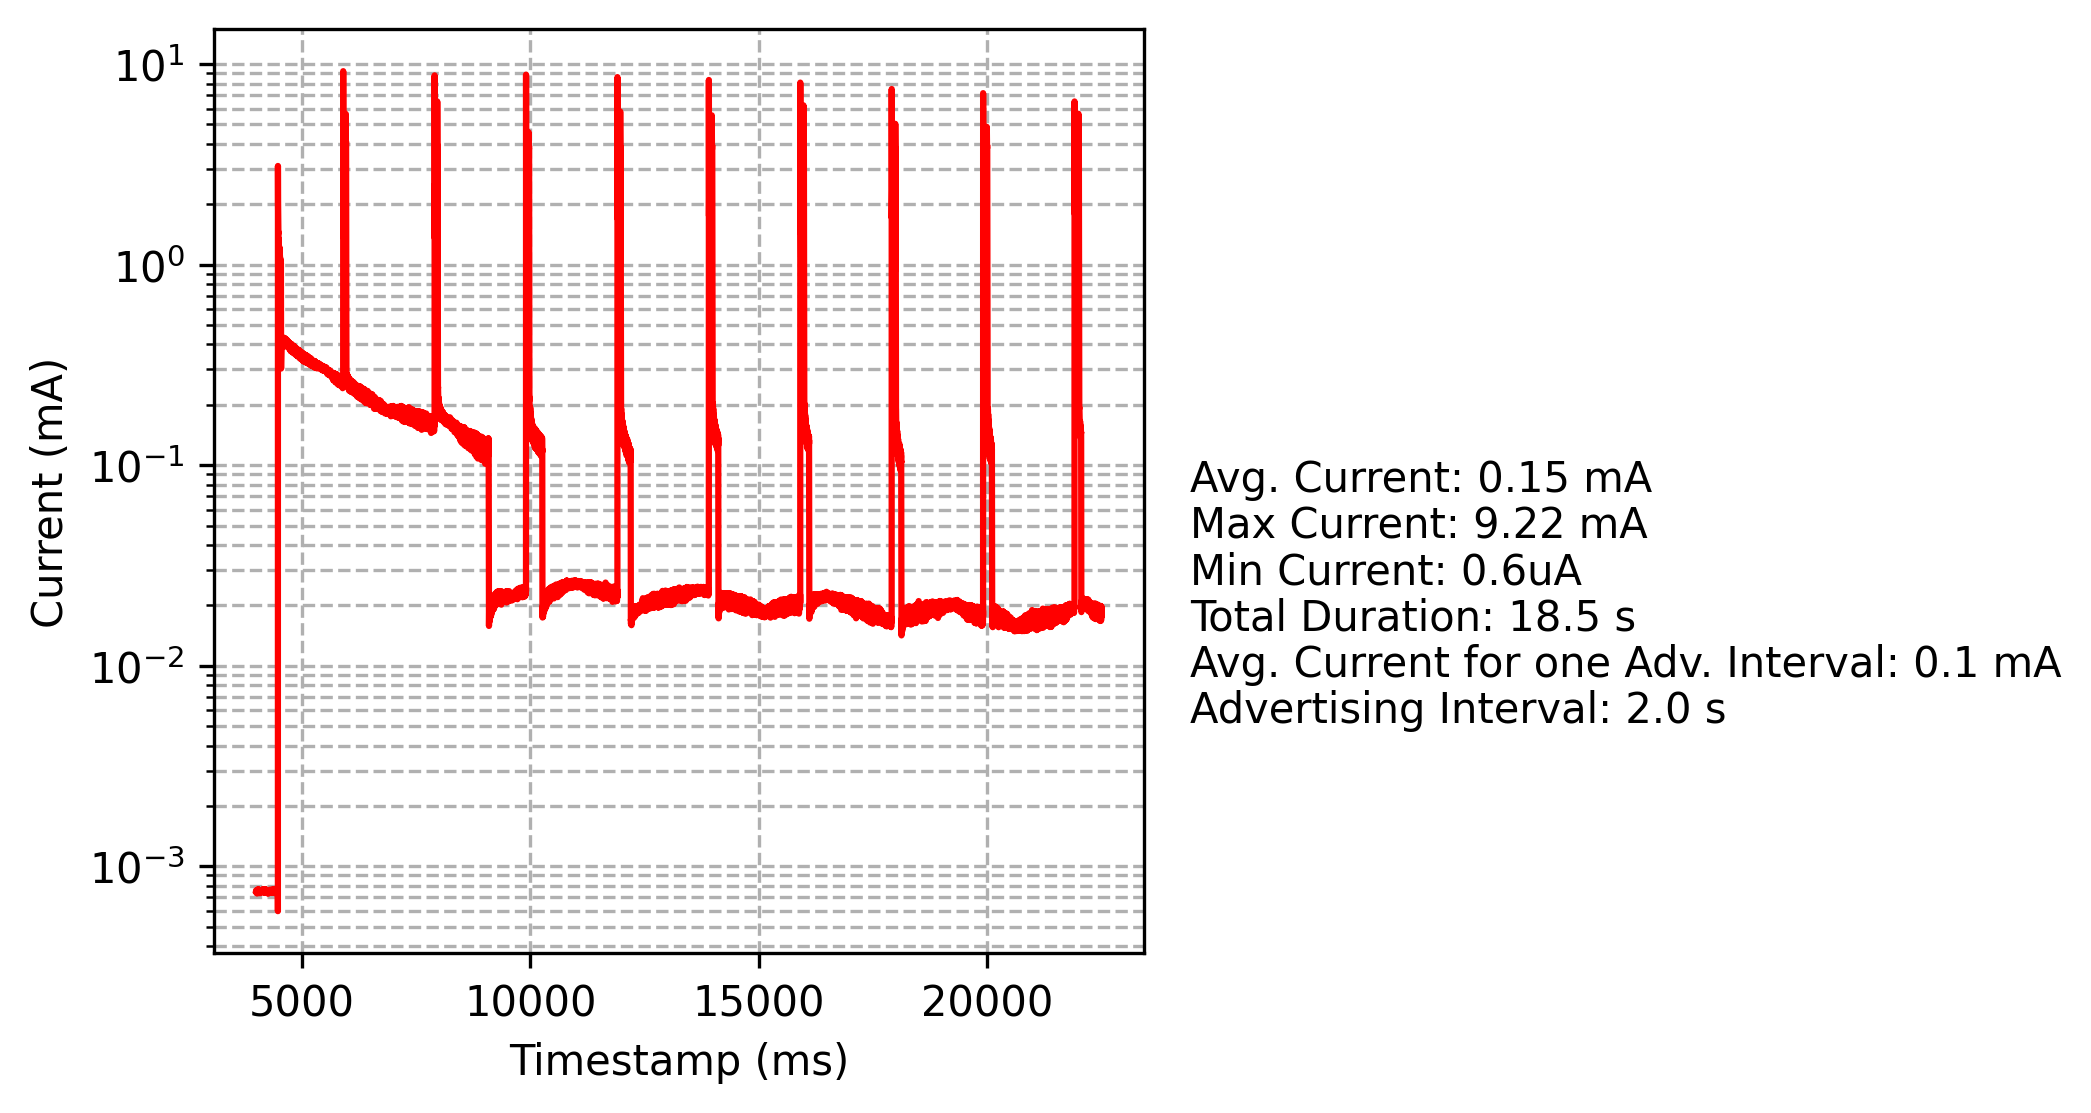
\includegraphics[width=0.8\linewidth]{chapters/Results/Current vs Timestamp - FreeBie Peripheral Medium.png}
        \caption{Current Measurement in Idle State - Peripheral}
        \label{fig:freebie_medium_peripheral}
    \end{subfigure}
    \begin{center}
        \begin{subfigure}{0.5\linewidth}
            \centering
            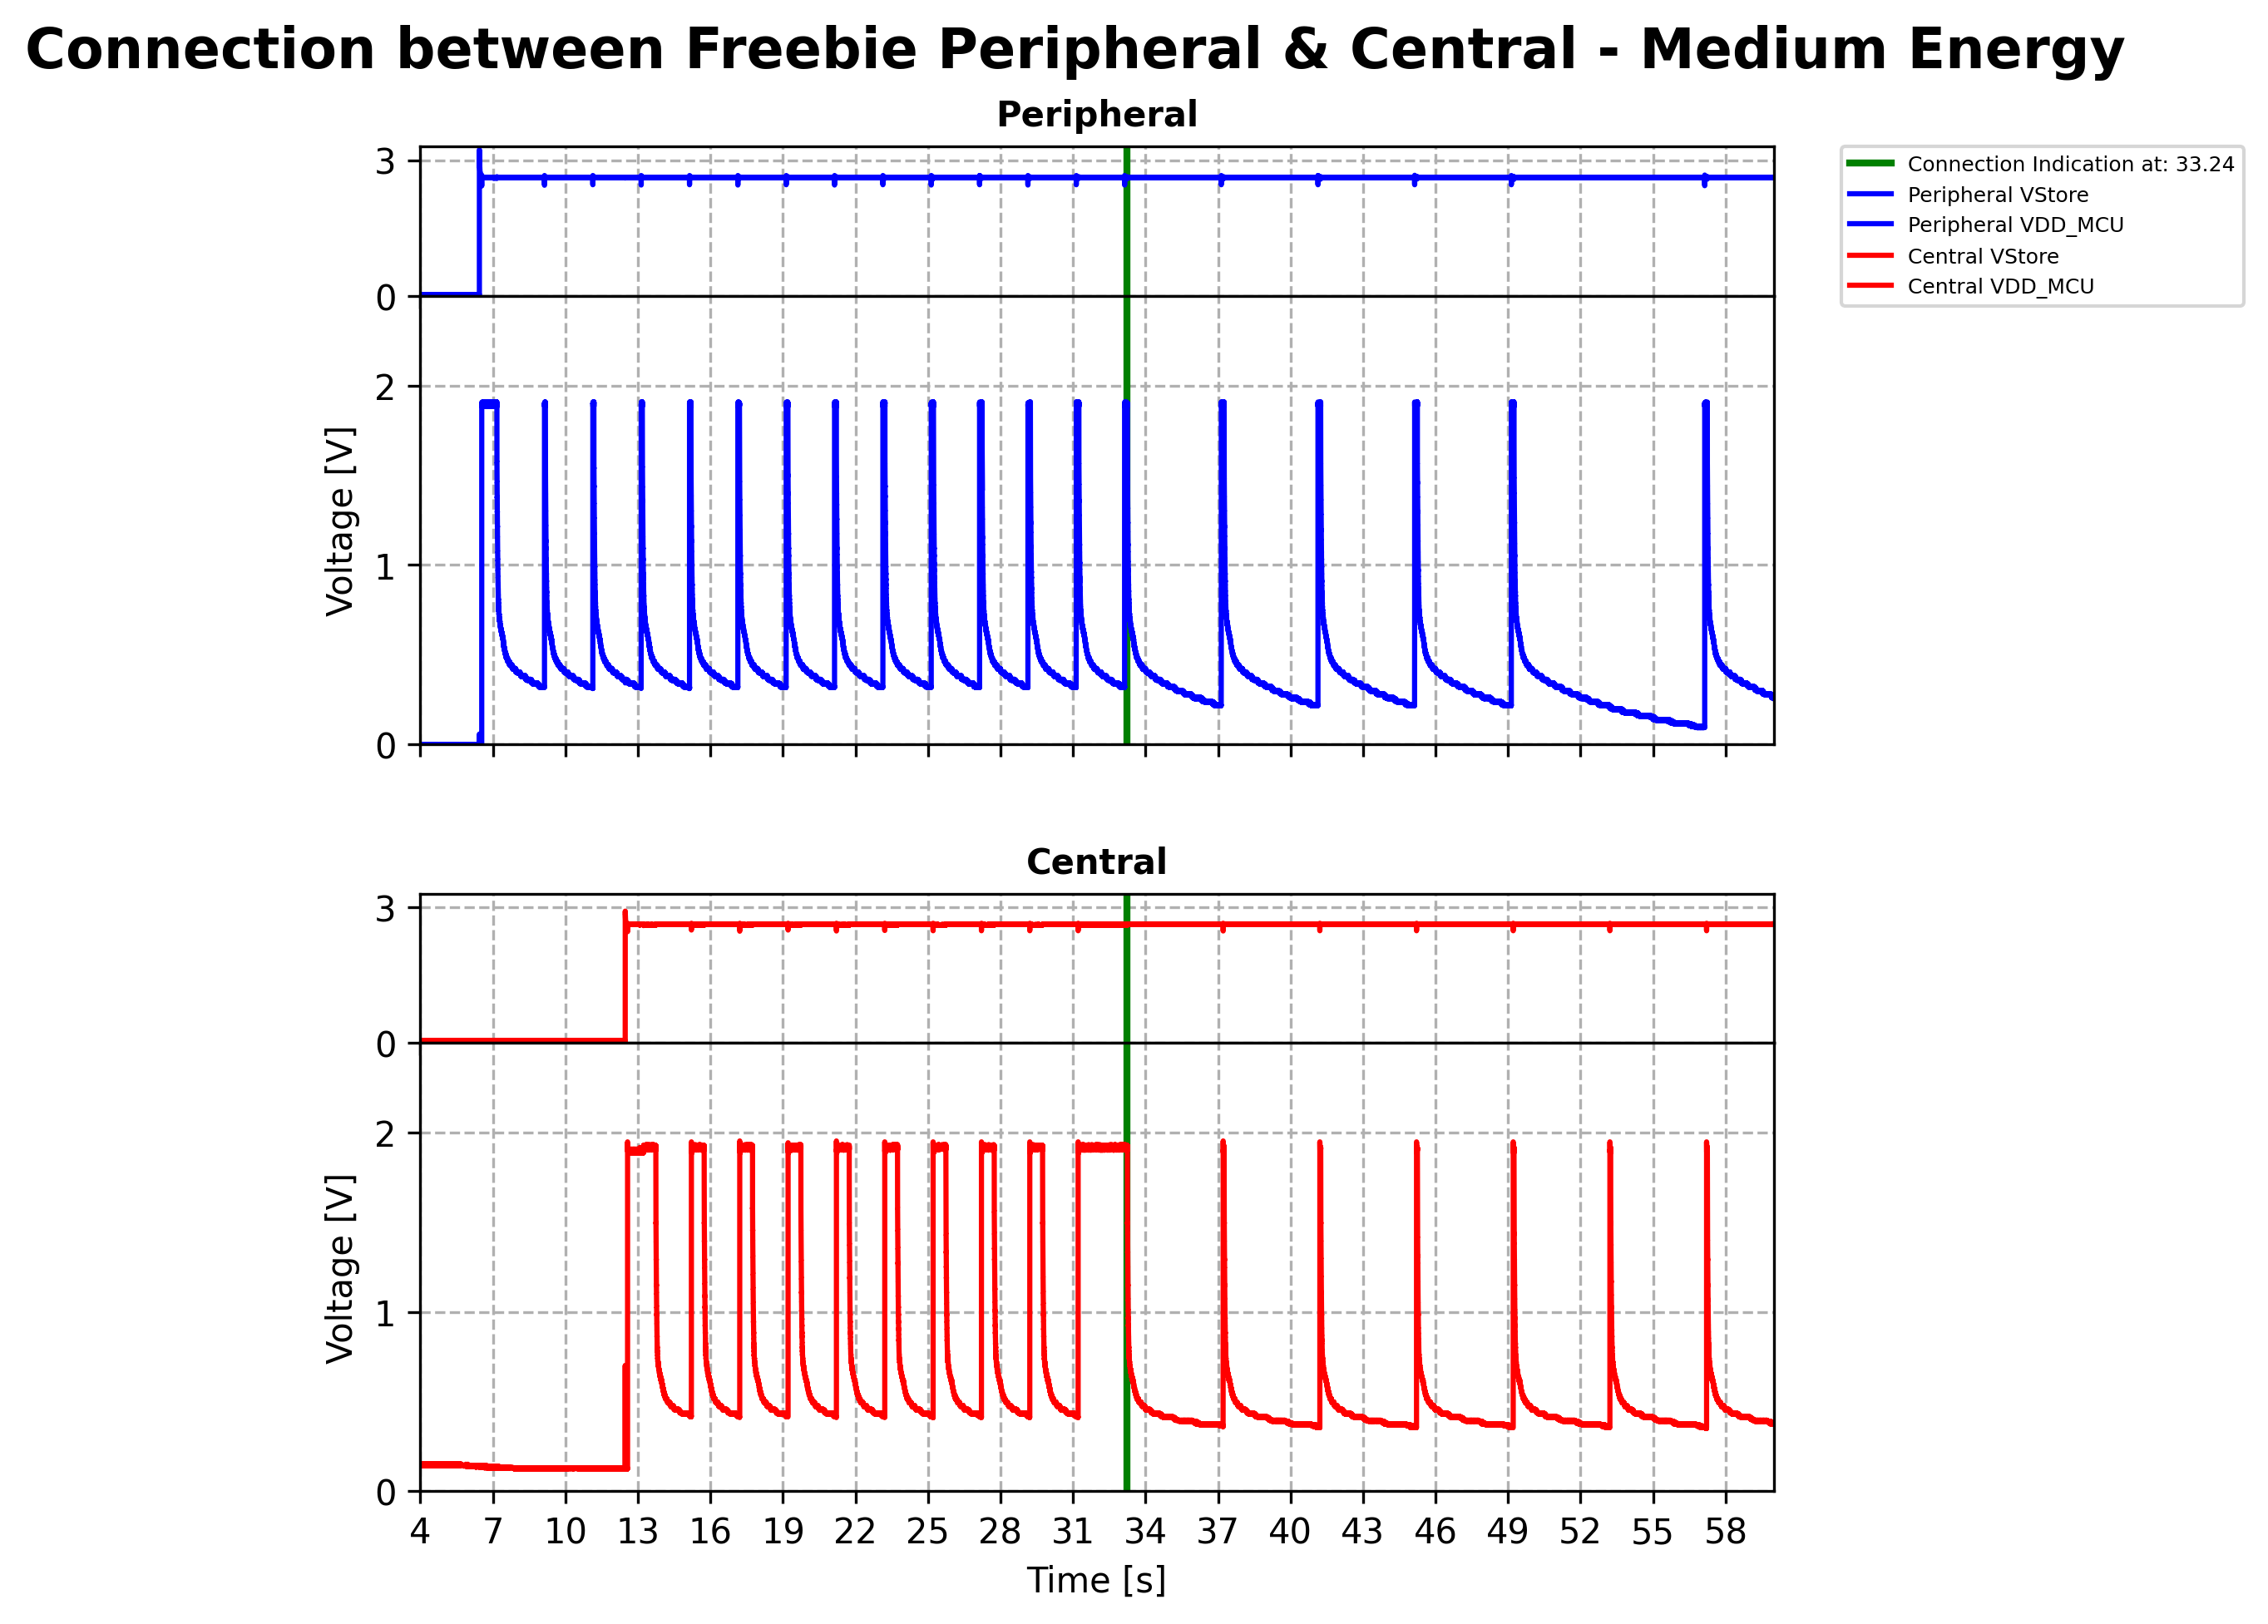
\includegraphics[width=\linewidth]{chapters/Results/Connection_Freebie_medium.png}
            \caption{Voltage Measurement trend exhibiting a successful BLE connection}
            \label{fig:freebie_medium_conn}
        \end{subfigure}    
    \end{center}
    \caption{\centering Time series plots showing behavior of FreeBie Medium system}
\end{figure}
\begin{figure}[H]
    \begin{subfigure}{0.5\linewidth}
        \centering
        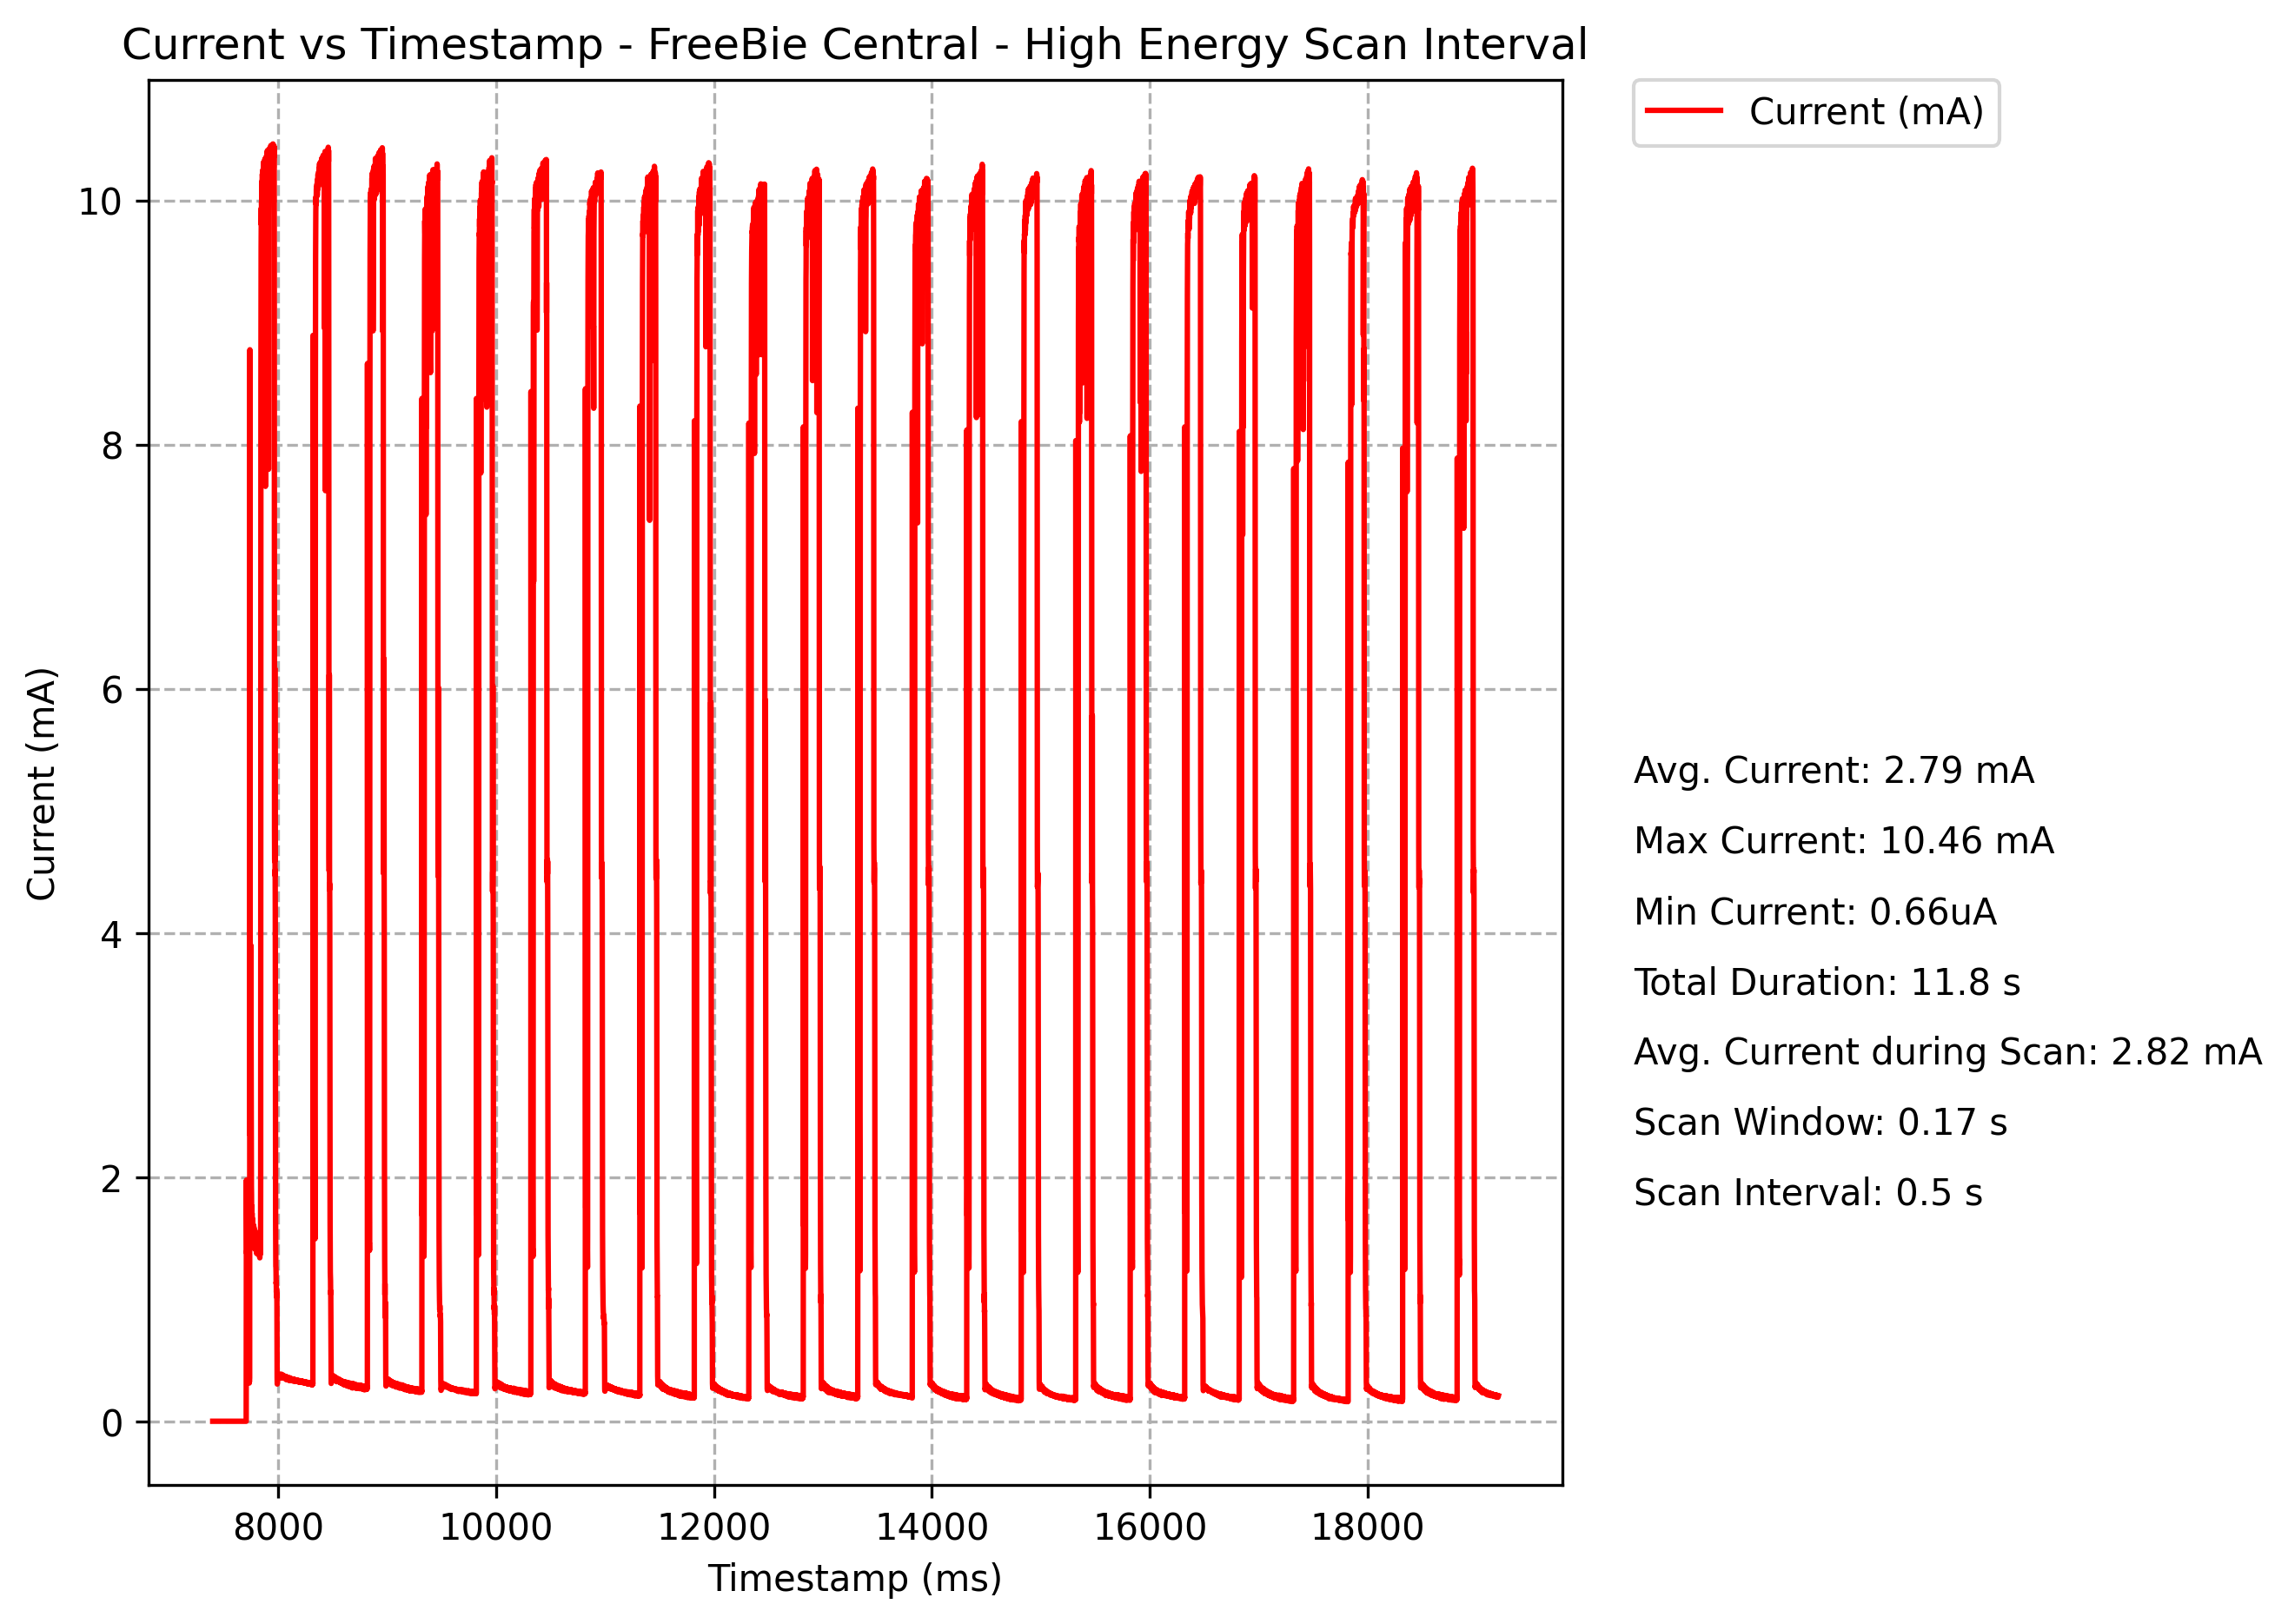
\includegraphics[width=0.8\linewidth]{chapters/Results/Current vs Timestamp - FreeBie Central High.png}
        \caption{Current Measurement in Idle State - Central}
        \label{fig:freebie_high_central}
    \end{subfigure}
    \begin{subfigure}{0.5\linewidth}
        \centering
        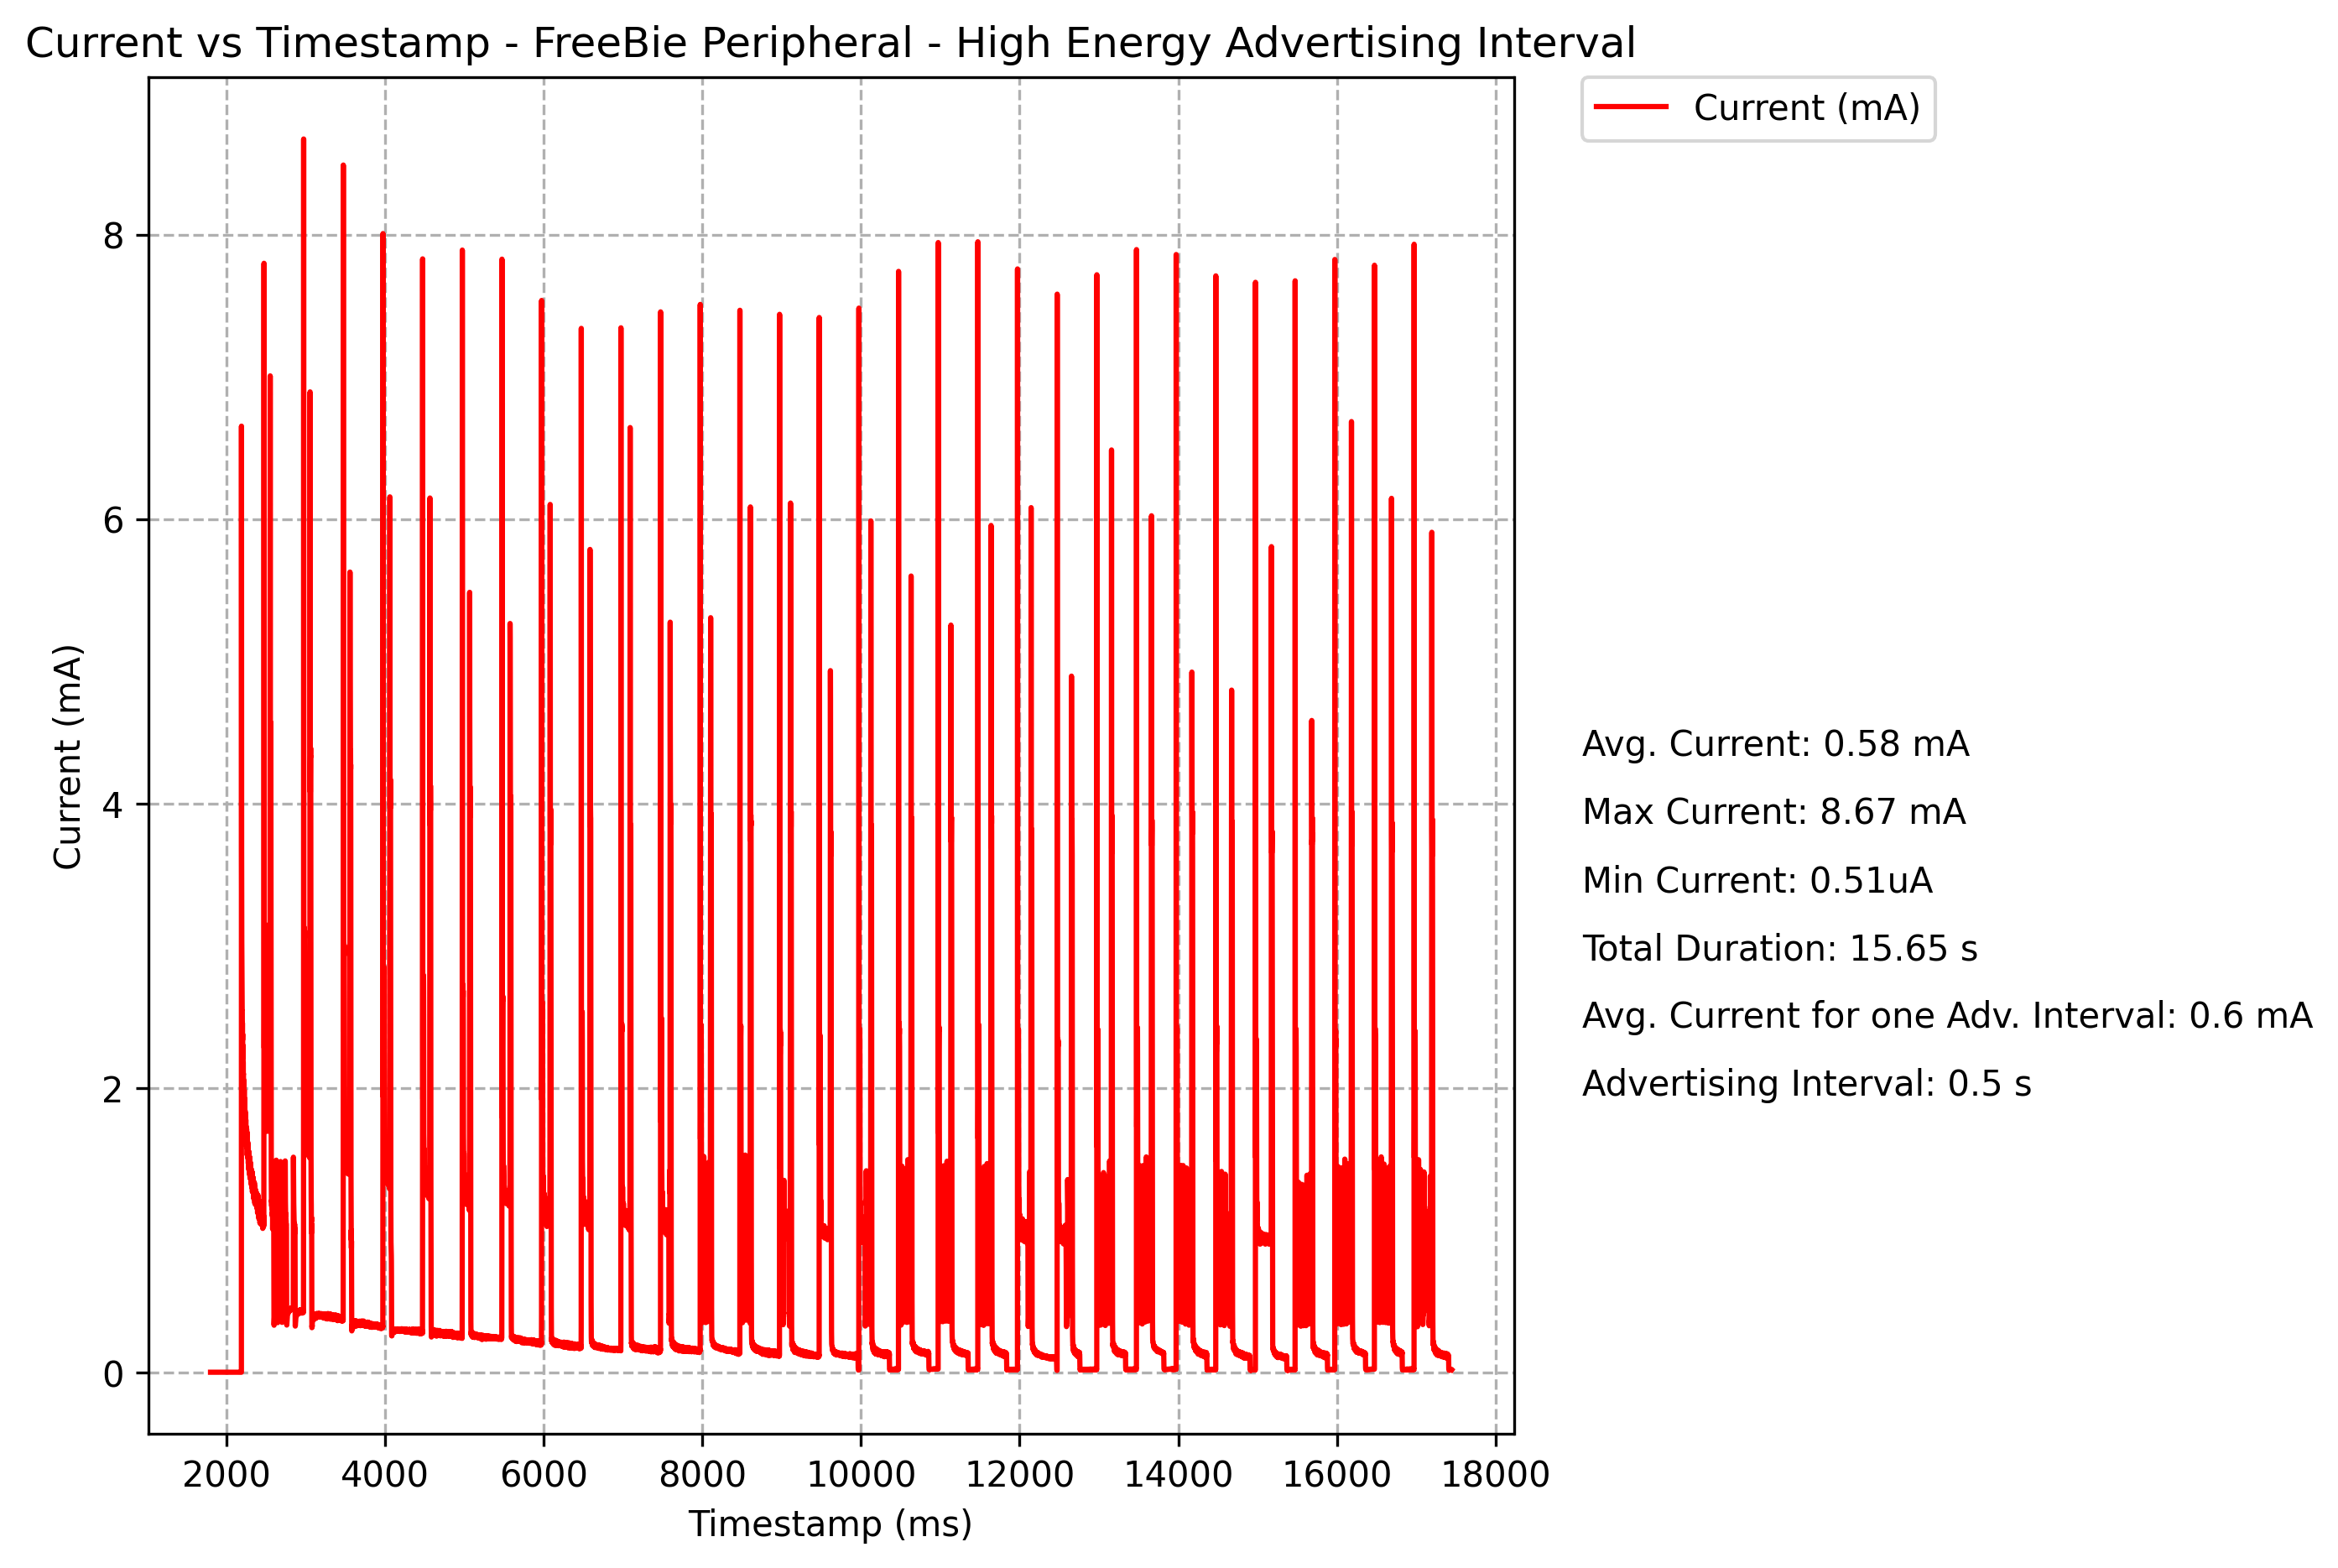
\includegraphics[width=0.8\linewidth]{chapters/Results/Current vs Timestamp - FreeBie Peripheral High.png}
        \caption{Current Measurement in Idle State - Peripheral}
        \label{fig:freebie_high_peripheral}
    \end{subfigure}
    \begin{center}
        \begin{subfigure}{0.5\linewidth}
            \centering
            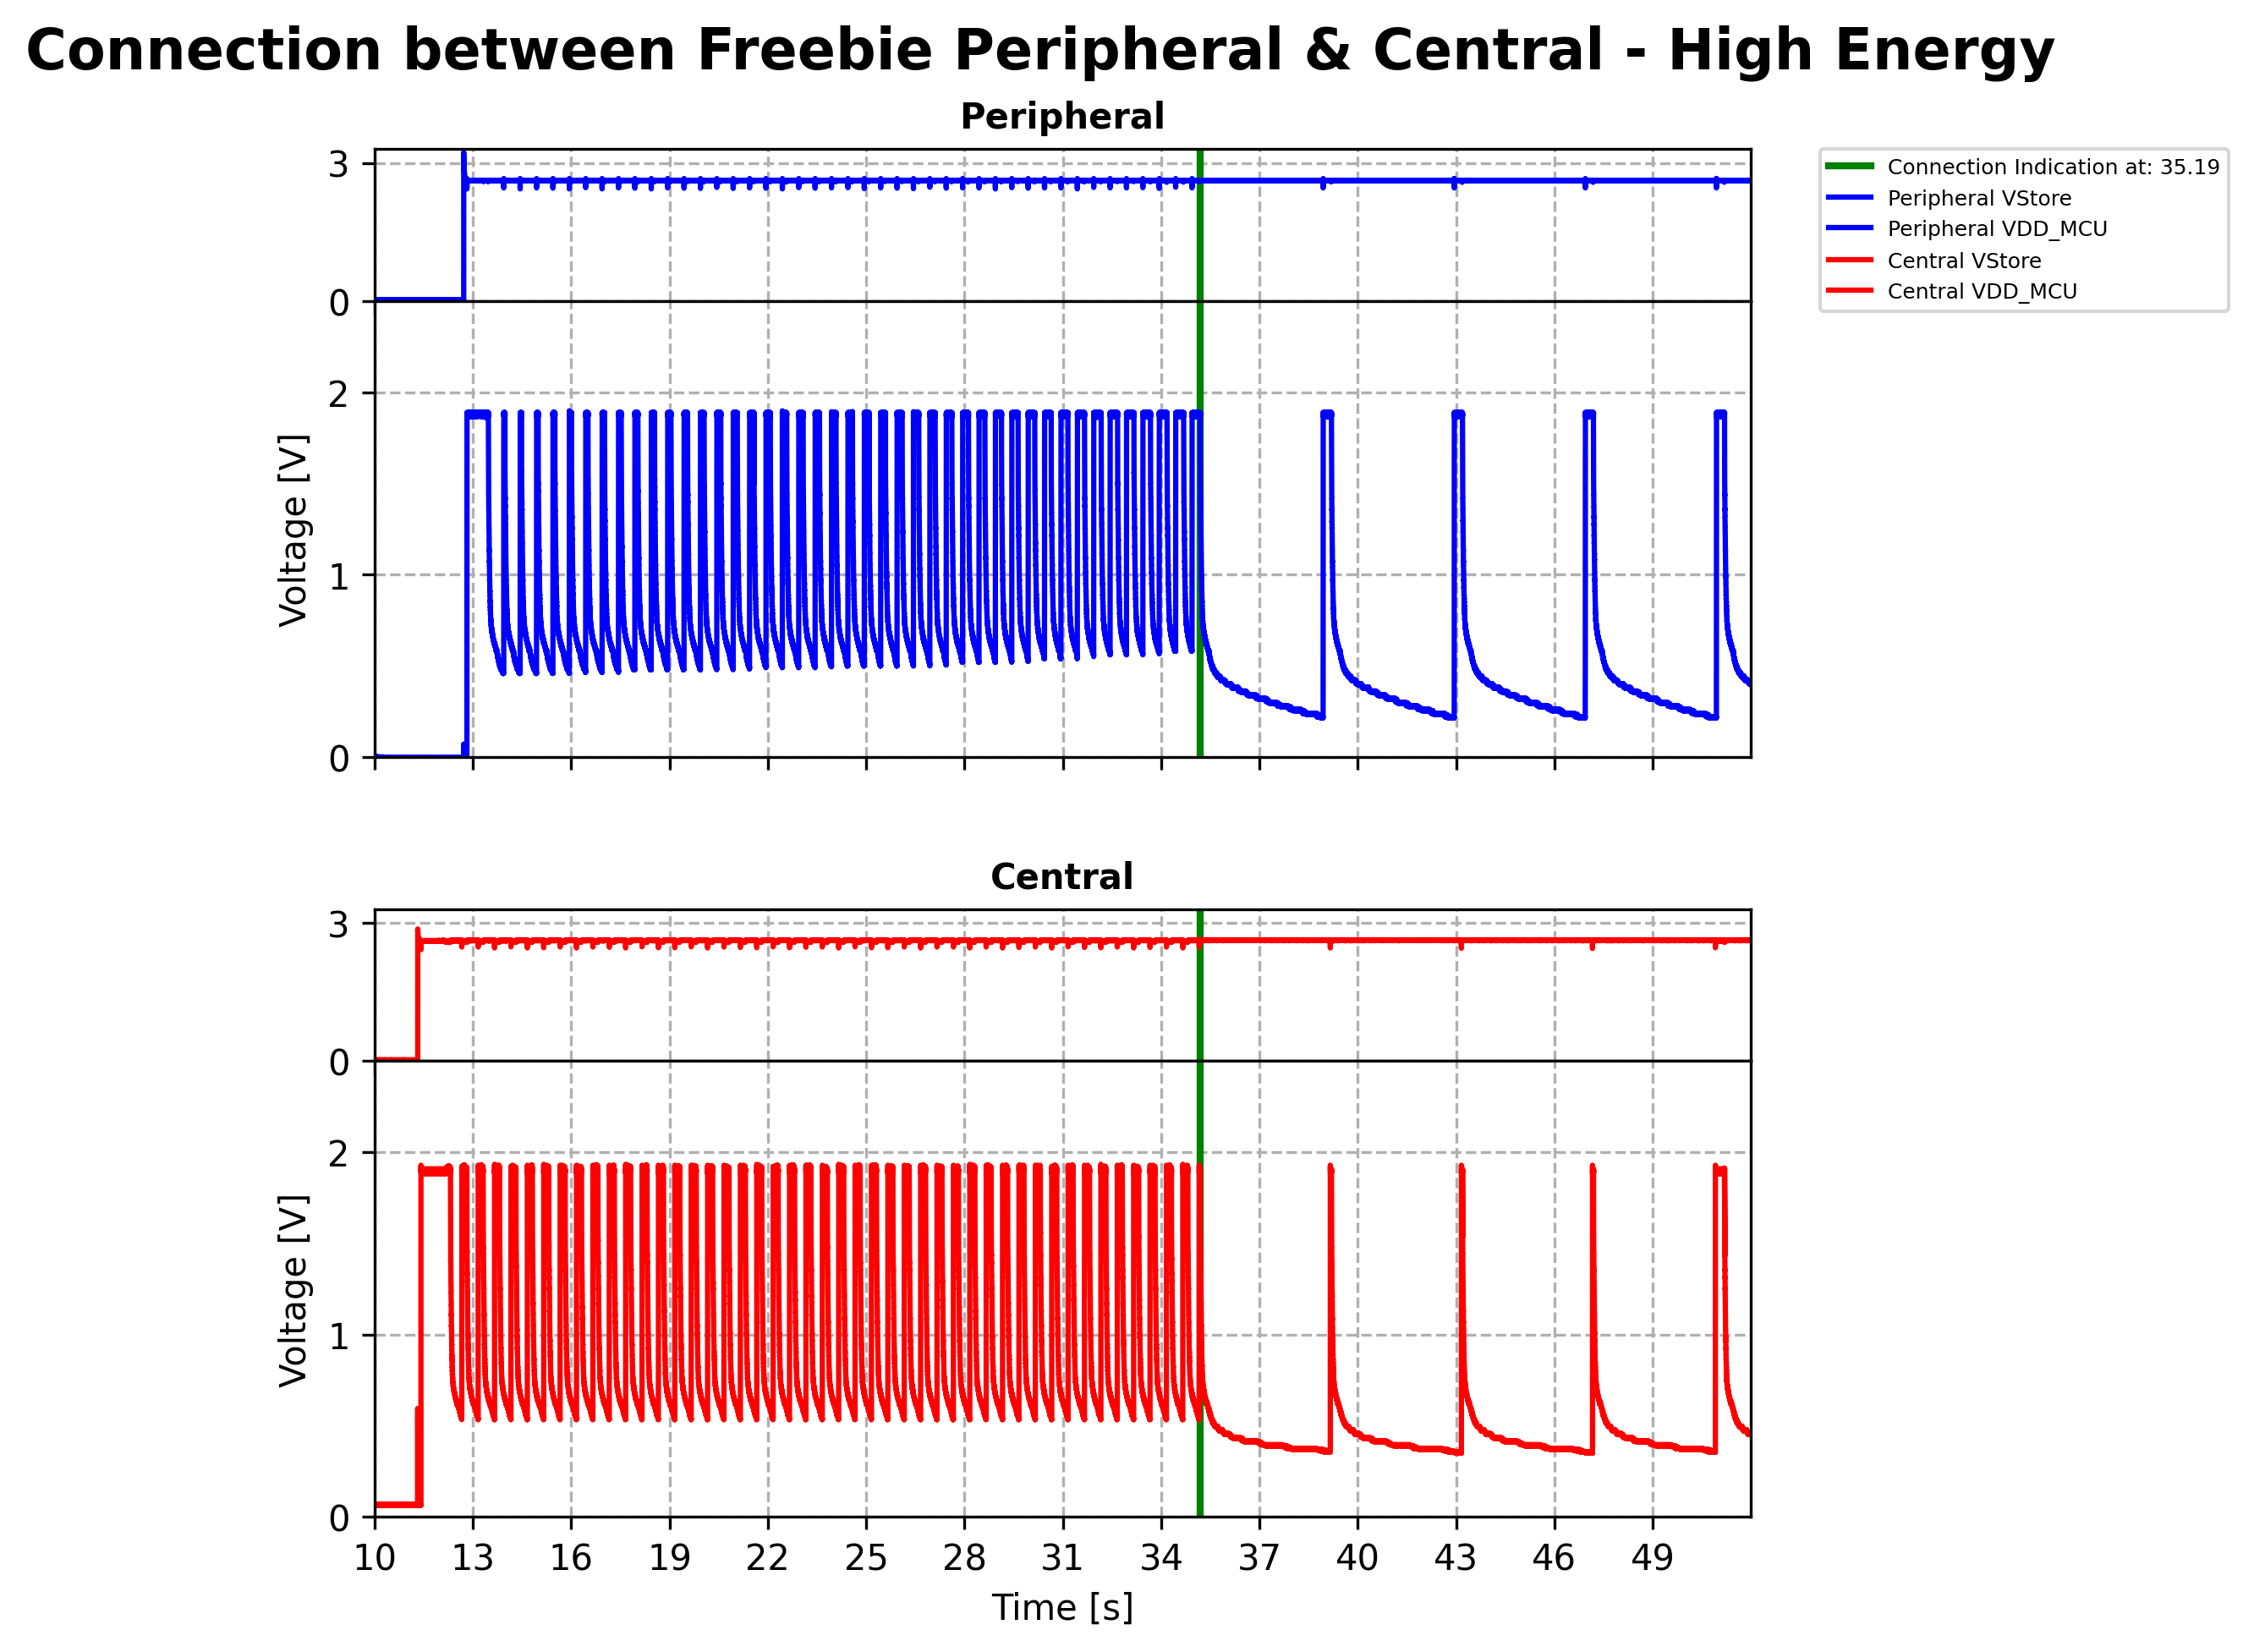
\includegraphics[width=\linewidth]{chapters/Results/Connection_Freebie_high.png}
            \caption{Voltage Measurement trend exhibiting a successful BLE connection}
            \label{fig:freebie_high_conn}
        \end{subfigure}    
    \end{center}
    \caption{\centering Time series plots showing behaviour of FreeBie High system}
\end{figure}

\subsection{Experimental Setup}
The experimental setup used in this study for comparative assessment is identical to the one stated in section \ref{sec:experimental_setup}. The experiment recorded the first connection setup time since boot-up for both the CardioSync system and the reference system separately. The measurement of sensor read time is also conducted in the context of the CardioSync system. The experiment was conducted a total of 20 times using the CardioSync device. In the context of the reference system, the experiment is iterated six times for each of the three distinct BLE configurations.

\noindent After data collection, the quantification of energy consumption becomes a focal point. The computation of energy expended by the device during each experiment, leading up to connection establishment, is achieved through the formula \[ \text{Energy (Joules)} = \text{Voltage} \times \text{Current} \times \text{Time taken to establish a connection}. \] Key parameters underpinning this calculation encompass the average current measured during distinct phases for both devices, coupled with the average voltage supply of 2.6 Volts. This quantitative analysis not only provides granular insights into energy utilization across experimental iterations but also serves as a crucial foundation for discerning the comparative efficiency and performance of the evaluated systems.


\subsection{Connection Setup Time Comparison}
The bar plot in Figure \ref{fig:conn_time_comp} graphically represents the average connection duration across different systems. Although CardioSync exhibits a slightly longer average connection time compared to the energy-efficient configuration of the reference FreeBie system, this distinction remains negligible. In contrast, juxtaposing CardioSync with FreeBie Medium and FreeBie High configurations reveals a notable enhancement in connection efficiency. Impressively, CardioSync achieves an average connection time \textbf{approximately 1.79 times faster than FreeBie Medium and roughly 1.65 times faster than FreeBie High}.

\noindent These comparisons emphasize CardioSync's capability to expedite connection establishment, particularly in comparison to the FreeBie Medium and FreeBie High configurations. Importantly, it should be noted that these comparisons derive from readings of the reference system intentionally synchronized by simultaneous activation. Without this deliberate synchronization, the reference system's BLE advertising and scanning intervals remain asynchronous, rendering it perpetually out of sync and unable to establish connections. Conversely, CardioSync achieves synchronization effortlessly, highlighting its distinct advantage.

\begin{figure}[H]
    \centering
    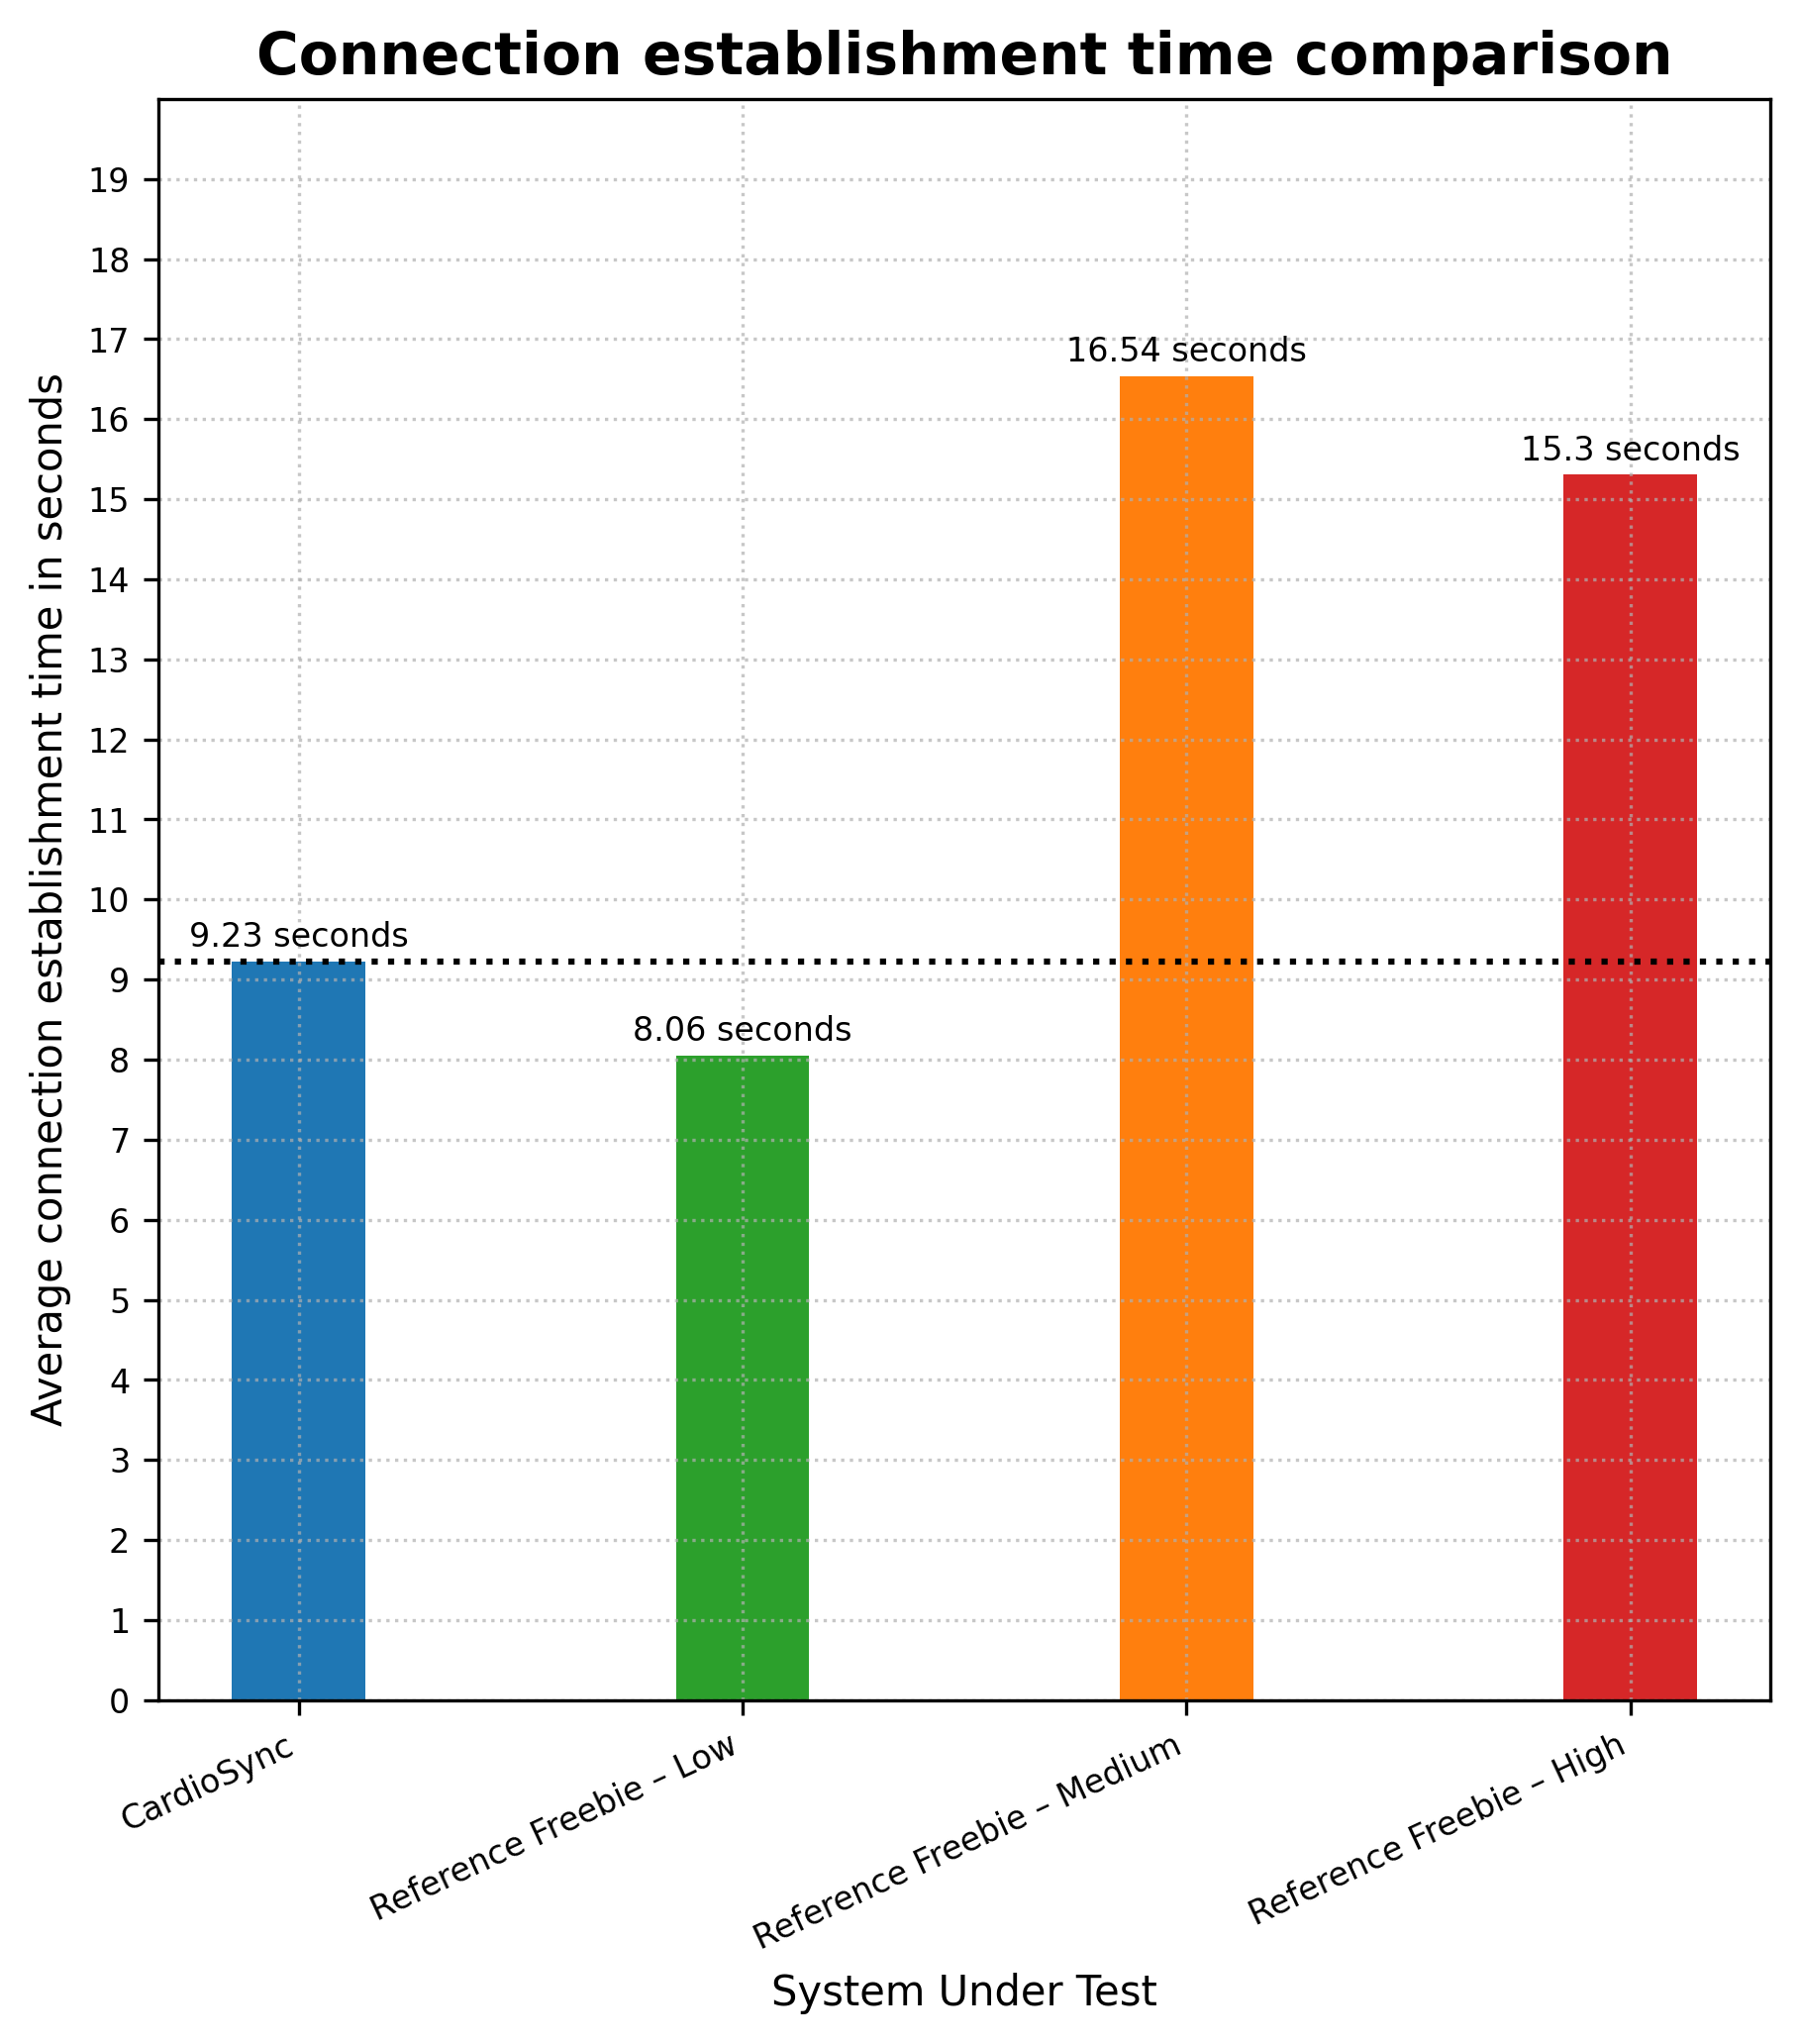
\includegraphics[width=0.8\linewidth]{chapters/Results/Connection_time_comparison.png}
    \caption{Bar plot showing Average BLE connection establishment time for each system for comparison}
    \label{fig:conn_time_comp}
\end{figure}


\subsection{Energy Consumption Comparison}
The barchart depicted in Figure \ref{fig:energy_comp} provides an illustrative view of the average energy expended to establish a connection for each system. Notably, CardioSync records an average energy consumption of 144.8 mJ, encompassing the cumulative energy consumption from boot-up, sensor initialization, active sensor reading, and heart rate-based sleep intervals. In contrast, the reference FreeBie systems exhibit significantly lower energy expenditures—27.51 mJ for FreeBie Low, 41.64 mJ for FreeBie Medium, and 68.04 mJ for FreeBie High.

\noindent Comparison of these results reveals that CardioSync consumes notably more energy compared to the reference FreeBie systems. This distinction is particularly evident when compared to FreeBie Low, where CardioSync's energy consumption is around 5.263 times higher. Similarly, when contrasted with FreeBie Medium and FreeBie High, CardioSync's energy consumption is approximately 3.48 and 2.13 times higher, respectively.

\noindent This observed energy disparity aligns with the inherent characteristics of CardioSync, wherein the integration of the MAX30102 sensor facilitates improved connection times through synchronized initial BLE connections. However, this enhanced performance comes at the trade-off of increased energy consumption. Furthermore, the partitioning of sensor energy consumption into distinct phases within the CardioSync system is depicted in the bar chart, showcasing the distribution of energy allocation for comprehensive insight.

\begin{figure}[H]
    \centering
    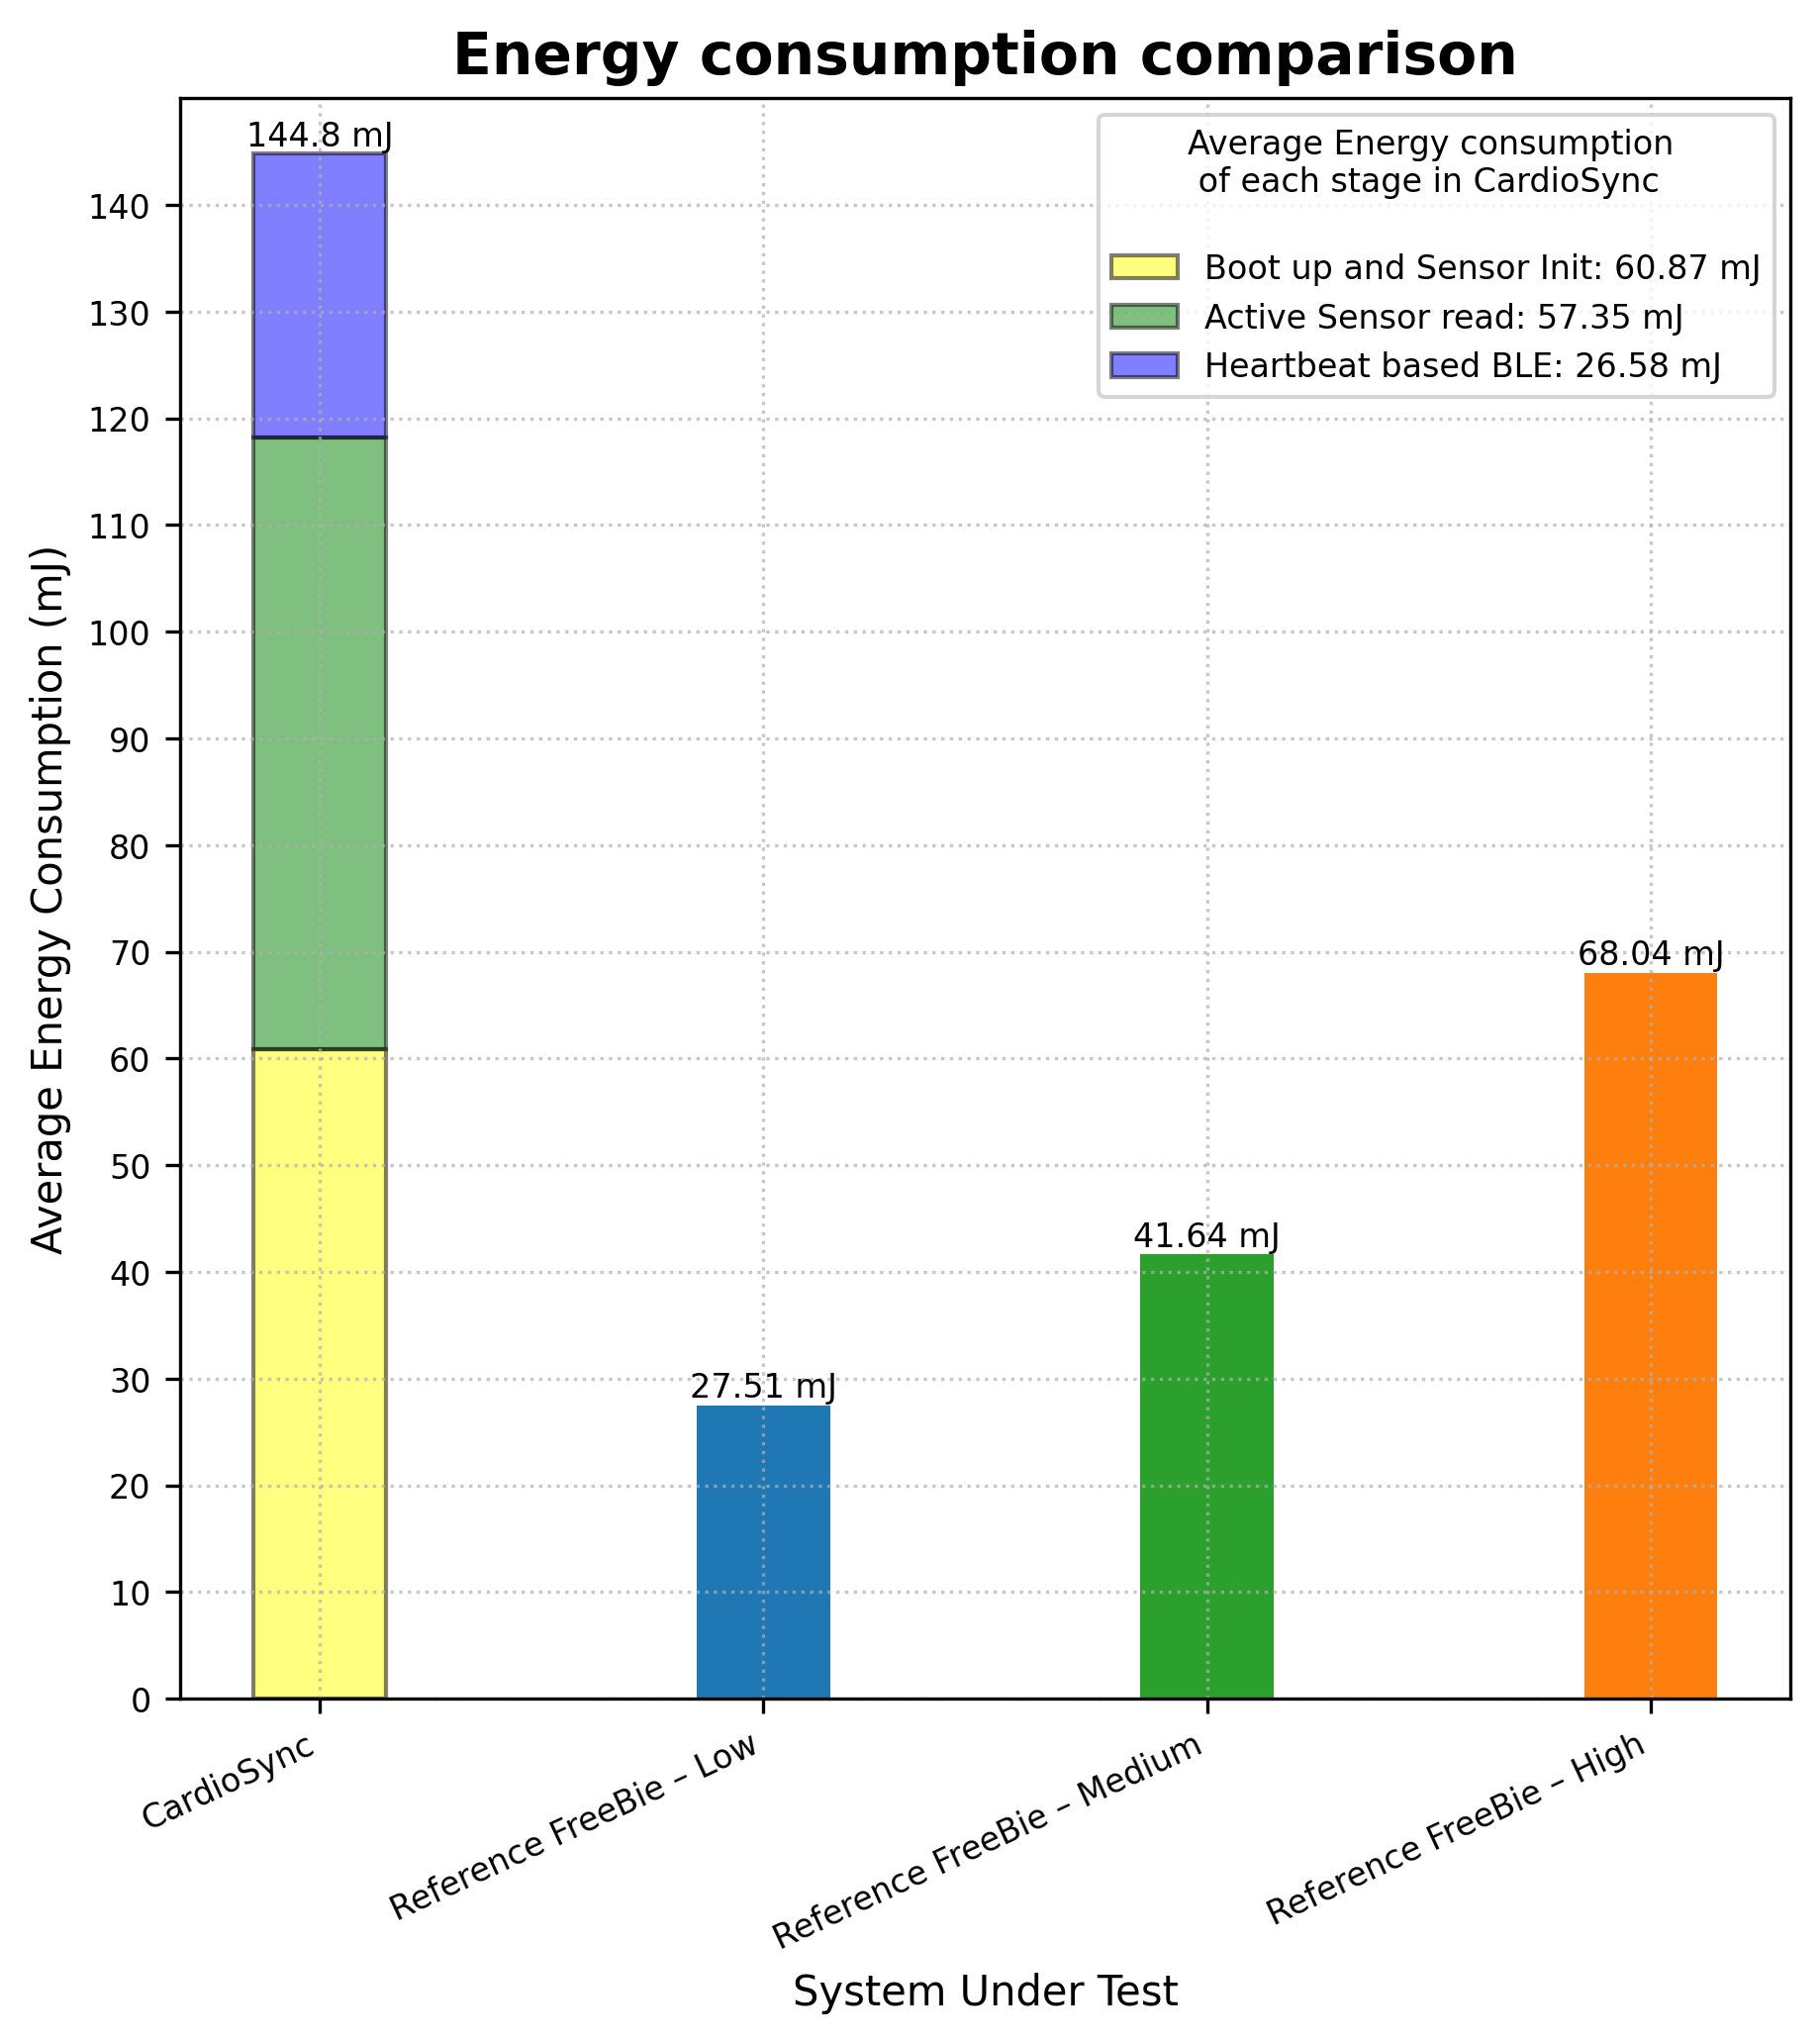
\includegraphics[width=0.7\linewidth]{chapters/Results/Energy_comparison.png}
    \caption{Bar plot showing Average energy consumed till connection setup for each system for comparison}
    \label{fig:energy_comp}
\end{figure}


\subsection{Power Comparison}
The bar chart depicted in Figure \ref{fig:power_comp} offers a visual representation of the average power expended to establish a connection for each system. Comparing these outcomes underscores that CardioSync consumes significantly more power when compared to the reference FreeBie systems. In comparison to FreeBie Low, CardioSync's power consumption is approximately 5.66 times higher. Similarly, in relation to FreeBie Medium and FreeBie High, CardioSync's power consumption is roughly 4.36 and 3.70 times higher, respectively. This power discrepancy mirrors the energy consumption pattern observed earlier and is congruent with the inherent trade-offs of the CardioSync system.

\begin{figure}[H]
    \centering
    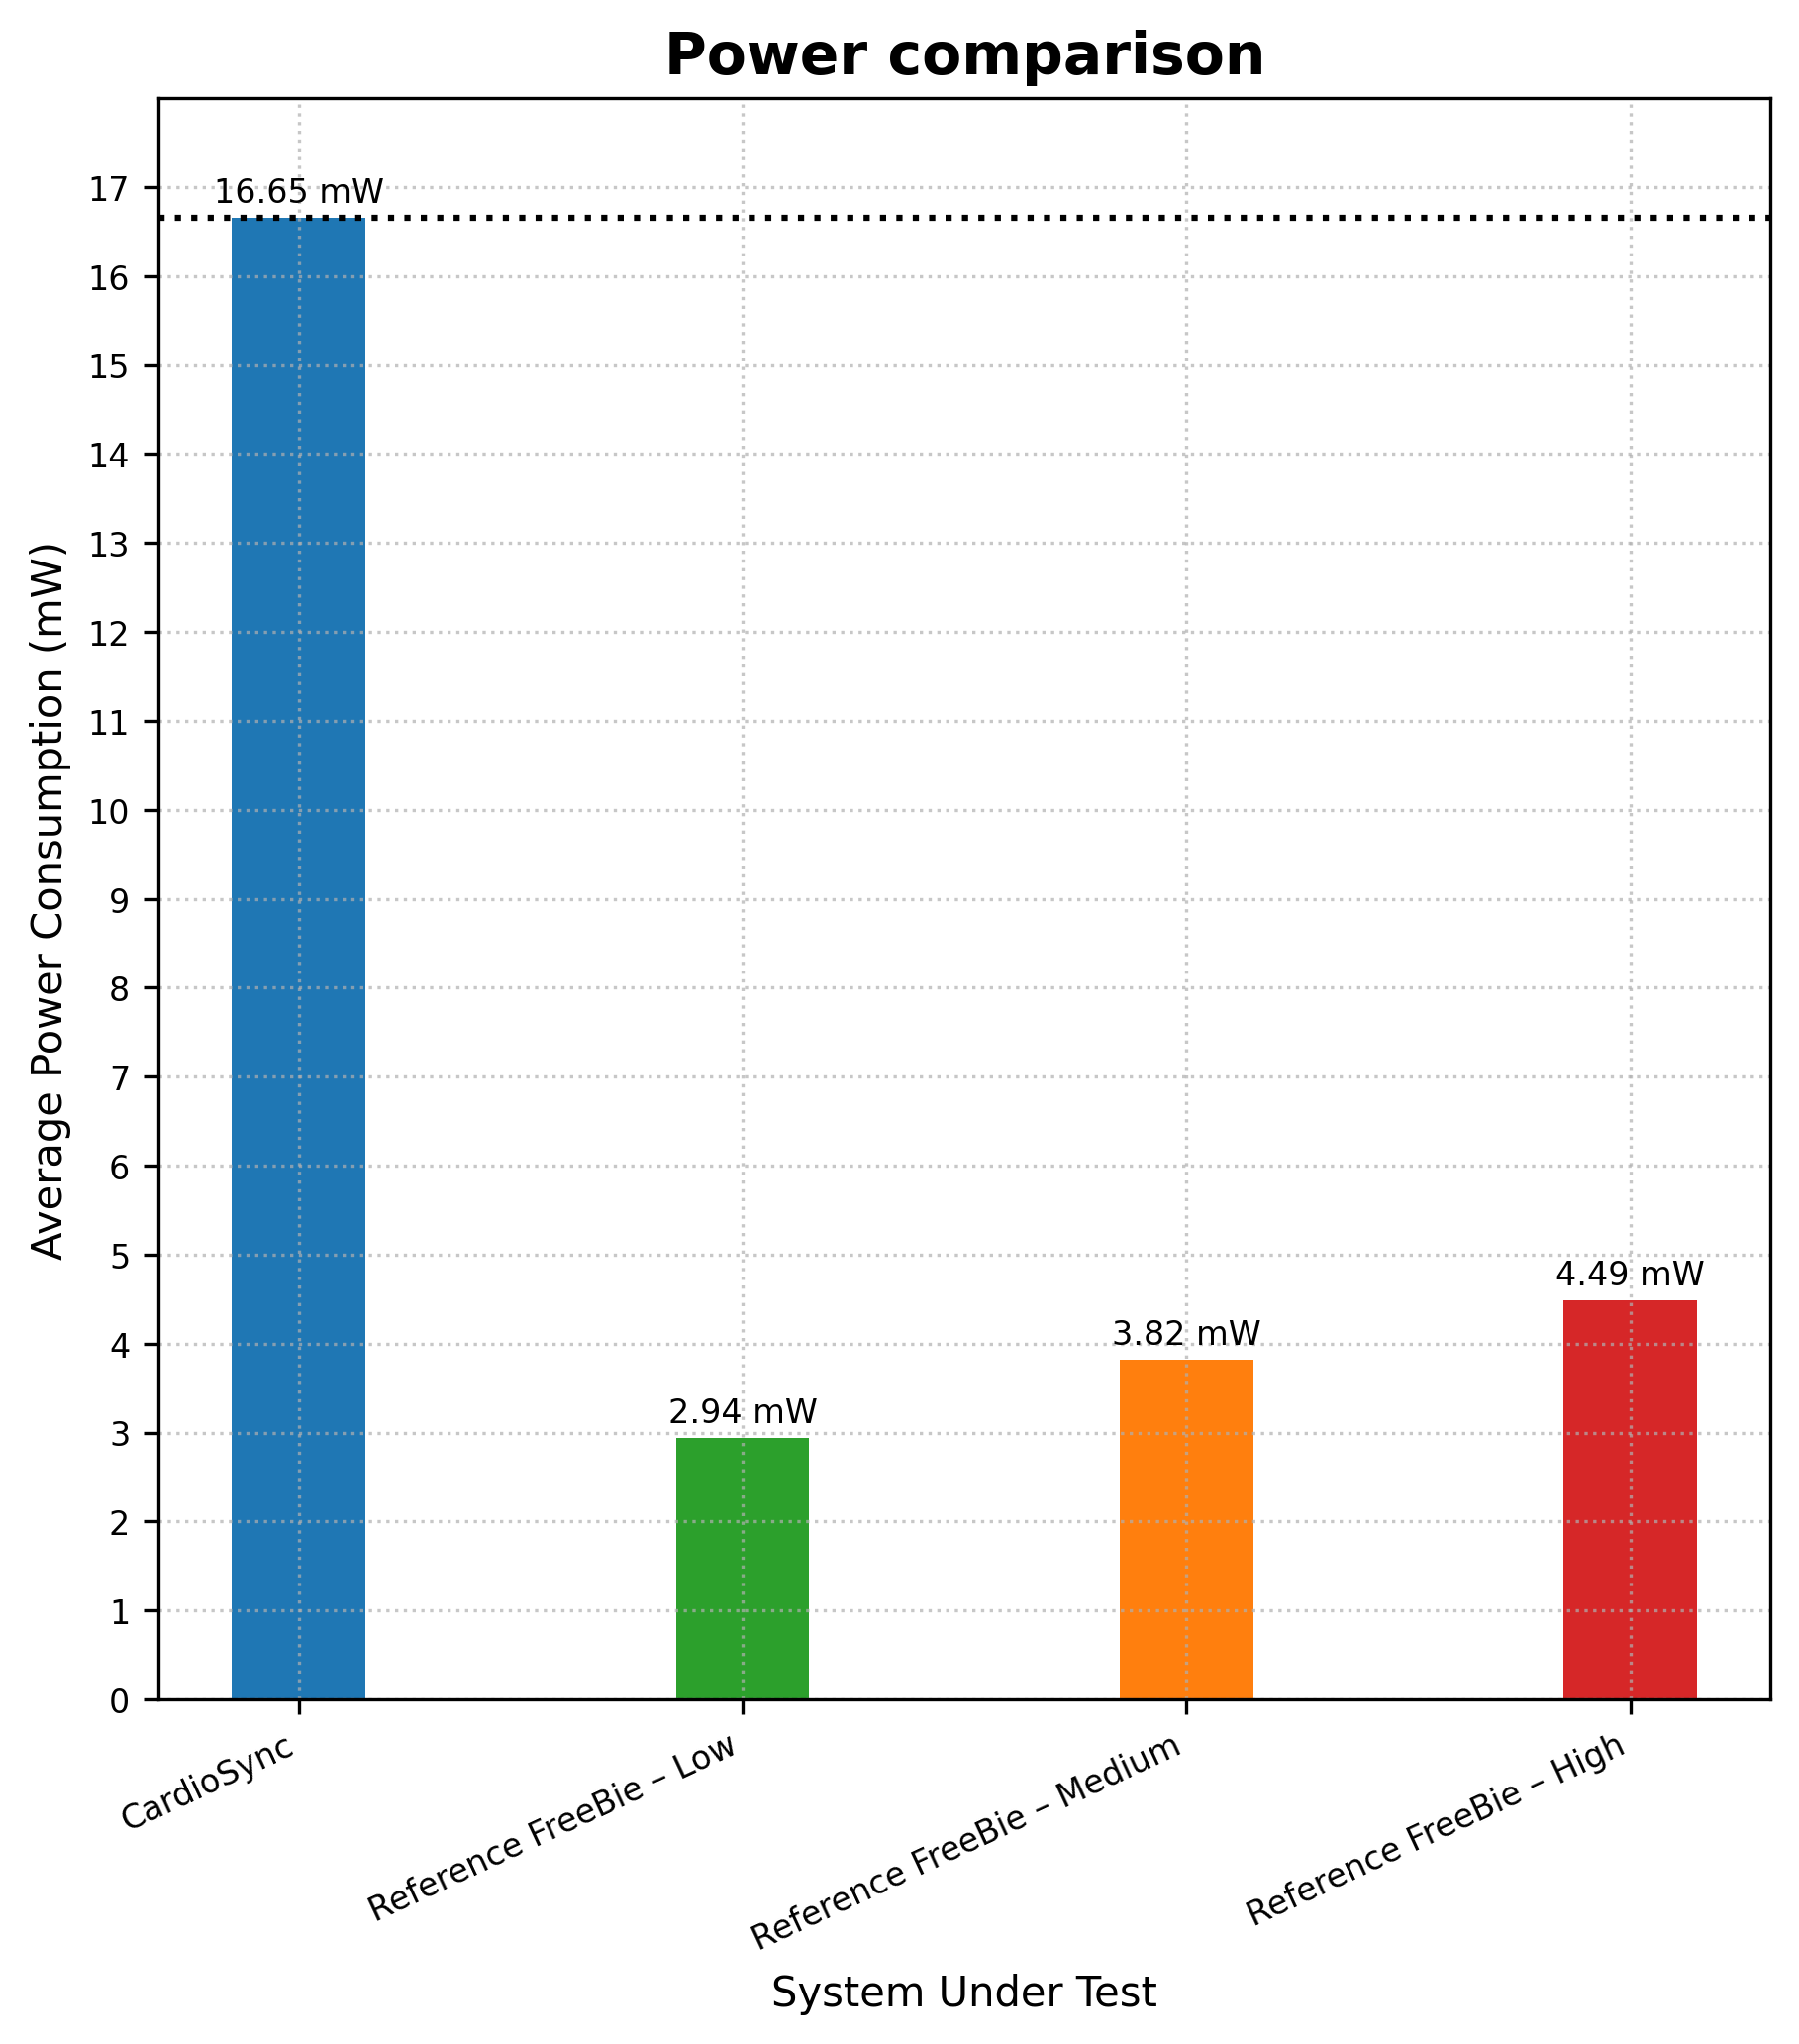
\includegraphics[width=0.7\linewidth]{chapters/Results/Power_comparison.png}
    \caption{Bar plot showing Average power consumed till connection setup for each system for comparison}
    \label{fig:power_comp}
\end{figure}

\subsection{Understanding Connection Setup Vs. Power}
The scatter plot in Figure \ref{fig:scatter_conn_power} presents an insightful juxtaposition of connection time against power consumption for both the CardioSync and reference FreeBie systems. Notably, the distribution of experimental data points for the CardioSync system predominantly converges in the upper left quadrant of the graph. This clustering signifies a higher power consumption alongside relatively shorter connection times. In contrast, the scatter plot depicting the reference FreeBie system showcases a more dispersed arrangement of data points, spanning across the lower half of the graph.

This disparity in data distribution emphasizes a pivotal distinction between the two systems. While the CardioSync system exhibits greater power consumption, it consistently achieves expedited connection times. In contrast, the reference FreeBie system, characterised by its asynchronous nature, demonstrates a wider range of connection times, contributing to the scattered data distribution in the scatter plot. This inconsistency in connection times, despite relatively lower power consumption, highlights the challenges inherent in achieving synchronisation within the battery-less FreeBie architecture.

In essence, the scatter plot serves as a visual testament to the trade-offs between power consumption and connection time. The CardioSync system, which has denser data points in the upper left quadrant, is an example of the potential advantages of utilising external synchronisation mechanisms to achieve consistent and effective connection times in a battery-free context.

\begin{figure}[H]
    \centering
    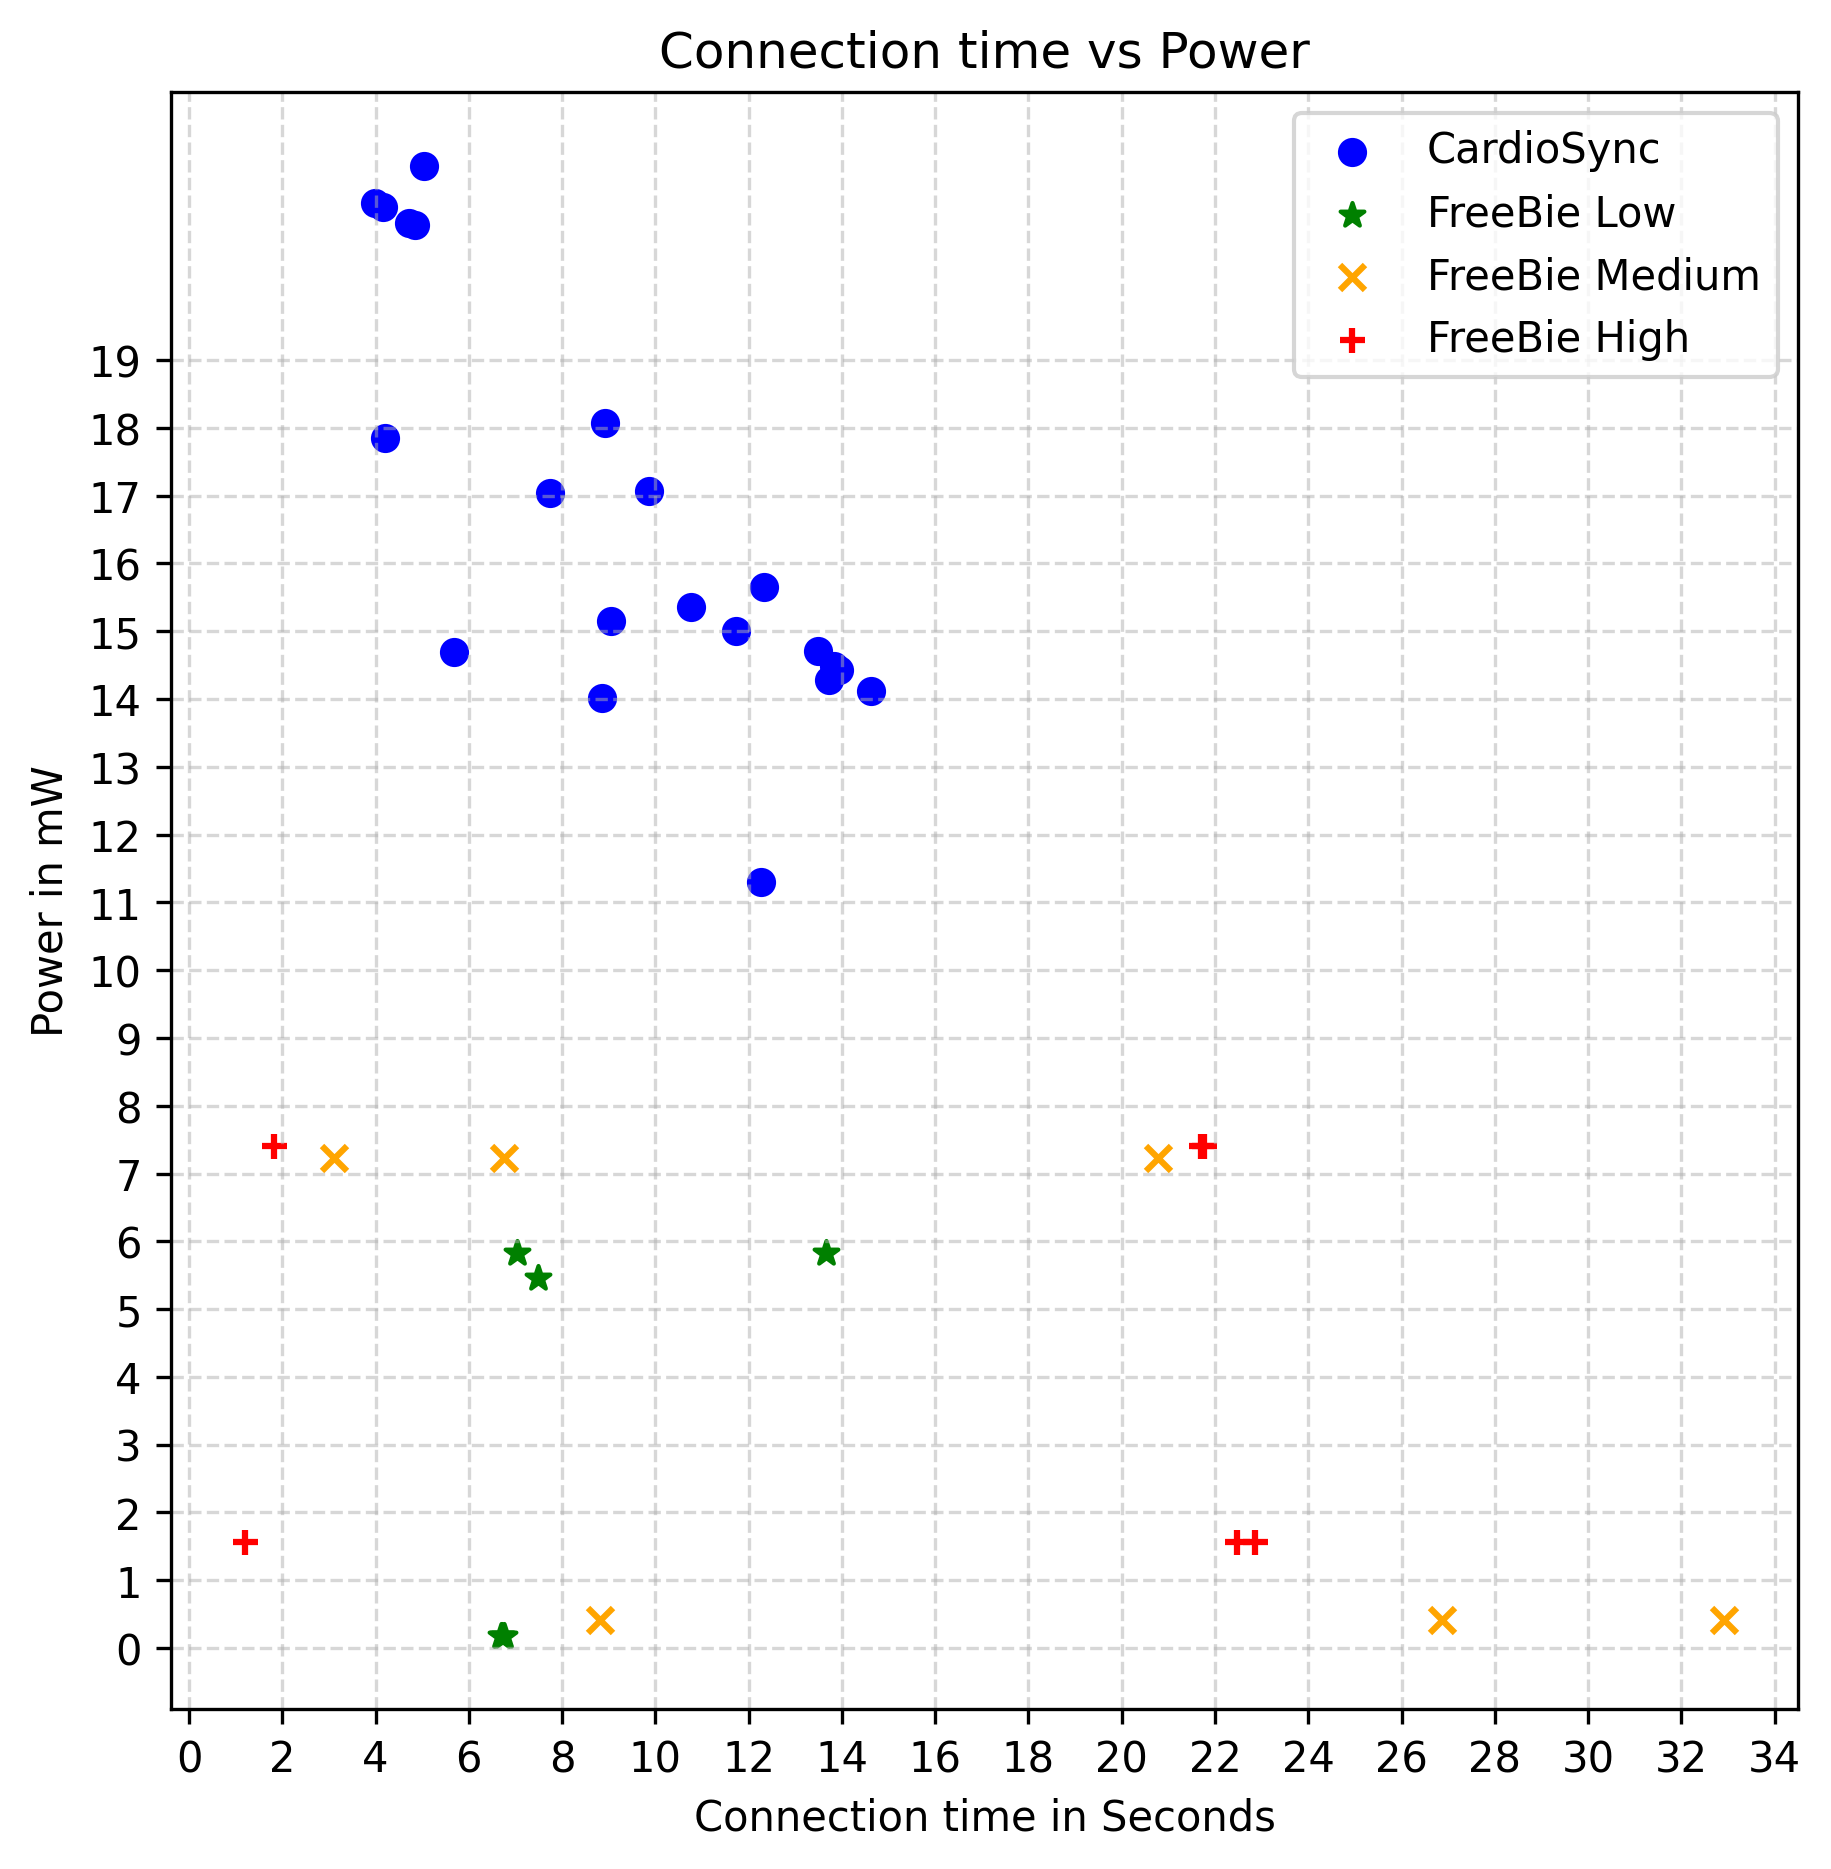
\includegraphics[width=0.7\linewidth]{chapters/Results/Scatter_plot.png}
    \caption{Scatter plot showing Connection time Vs. Power}
    \label{fig:scatter_conn_power}
\end{figure}

\section{Discussion of Key Findings}
In this section, we delve into the implications and insights derived from the comparative analysis between the newly developed CardioSync framework and the reference FreeBie system. The evaluation encompassed power, energy, and connection time dynamics, shedding light on the system's performance and potential trade-offs.

\begin{itemize}
    \item \textbf{Power and Energy Efficiency:} CardioSync framework exhibited a higher connection time efficiency; however, this gain was balanced by higher power and energy expenditure. CardioSync This can be attributed to the deliberate inclusion of the MAX30102 sensor for synchronisation, which inherently demands additional energy resources.

    \item \textbf{Connection Time and Synchronization:} A significant standout was CardioSync's consistent achievement of reduced connection times. In contrast, the reference FreeBie system displayed a broader spectrum of connection times, reflecting its asynchronous nature. While FreeBie's power consumption remained lower, the scatter plot underscored the inherent challenges of maintaining synchronisation within the battery-less framework.

    \item \textbf{Trade-Offs and Implications:} CardioSync's elevated energy usage, albeit resulting in enhanced connection times, introduces trade-offs that necessitate careful consideration in real-world applications. The reference FreeBie system's dispersed connection times highlight the inherent difficulty of achieving synchronisation without specialized mechanisms.
\end{itemize}

Collectively, the meticulous evaluation of CardioSync against the reference FreeBie system strategically aligns with our research objectives and validates the achievement of our research goals, effectively enhancing the discourse and possibilities within the battery-less domain.


% Advancements and Future Directions
% The exploration and evaluation conducted here serve as a foundational stepping stone. The insights gained pave the way for potential advancements in synchronization strategies and energy-efficient connectivity. Further investigations could explore fine-tuned sensor utilization strategies, optimizing power usage without compromising connection times.

% These results underscore the complexities inherent in designing battery-less embedded systems. While the CardioSync system boasts impressive synchronization accuracy through heart rate-based synchronization, the Freebie system shines in energy and power efficiency. The choice between the two systems depends on the specific application requirements, where precision or conservation may hold precedence.

% In the subsequent section, we delve deeper into the implications and significance of these results, discussing their practical implications and providing insights into the potential future directions of this research.